%%%%%%%%%%%%%%%%%%%%%%%%%%%%%%%%%%%%%%%%%%%%%%%%%%%%%%%%%%%%%%%%%%%
%%% Documento LaTeX 											%%%
%%%%%%%%%%%%%%%%%%%%%%%%%%%%%%%%%%%%%%%%%%%%%%%%%%%%%%%%%%%%%%%%%%%
% Título:	Plantilla de TFG/TFM
% Autor:  Ignacio Moreno Doblas
% Fecha:  2014-02-01, actualizado 2019-11-11
%%%%%%%%%%%%%%%%%%%%%%%%%%%%%%%%%%%%%%%%%%%%%%%%%%%%%%%%%%%%%%%%%%%
%	Modo:					PDFLaTeX.
%%%%%%%%%%%%%%%%%%%%%%%%%%%%%%%%%%%%%%%%%%%%%%%%%%%%%%%%%%%%%%%%%%%

% Preámbulo del documento.
%-----------------------------------------------------------------%
% Clase de documento: libro
\documentclass[12pt,a4paper]{book} % article, report, book.

% Preámbulo: paquetes, comandos, entornos, estilos y título de página.
%%%%%%%%%%%%%%%%%%%%%%%%%%%%%%%%%%%%%%%%%%%%%%%%%%%%%%%%%%%%%%%%%%%
%%% Documento LaTeX 																						%%%
%%%%%%%%%%%%%%%%%%%%%%%%%%%%%%%%%%%%%%%%%%%%%%%%%%%%%%%%%%%%%%%%%%%
% Título:	Paquetes
% Autor:  Ignacio Moreno Doblas
% Fecha:  2014-02-01, actualizado 2019-11-11
%%%%%%%%%%%%%%%%%%%%%%%%%%%%%%%%%%%%%%%%%%%%%%%%%%%%%%%%%%%%%%%%%%%
% Tabla de materias:
%	1 Codificación e idioma %
% 2 Matemáticas y Física %
% 3 Gráficos%
% 4 Estilo y formato%
%%%%%%%%%%%%%%%%%%%%%%%%%%%%%%%%%%%%%%%%%%%%%%%%%%%%%%%%%%%%%%%%%%%

%1 Codificación e idioma%
\usepackage[utf8]{inputenc} %Codificación en latin-1%
\usepackage[T1]{fontenc} %Codificación de fuente%
\usepackage[spanish]{babel}	%Hyphenation (Guionado) en español%
\usepackage{eurosym} %Tipografía euro (€)%

%2 Matemáticas y Física %
% Importante para ecuaciones, magnitudes y unidades%
\usepackage{amssymb,amsmath,latexsym,amsfonts} % paquetes estándar%
\usepackage[squaren]{SIunits} %Paquete para magnitudes y unidades físicas%
\usepackage{ifthen} %sentencias if y while%

%3 Gráficos%
\usepackage{graphics,graphicx,subcaption} %paquetes gráficos estándar%
%\usepackage{subfigure} %permite varias subfiguras en una figura
\usepackage{wrapfig} %paquete para gráfica lateral%
\usepackage{float} %figuras flotantes%
	% \begin{floatingfigure}[r]/[l]{4.5cm}
	% \end{floatingfigure}
\usepackage{graphpap}	%comando \graphpaper en el entorno picture%

%4 Estilo y formato%
\usepackage{imakeidx} %MakeIndex%
%Comando para crear glosario (index en inglés)
\makeindex[columns=2, title=Glosario, intoc]
%\usepackage{showidx} % Hace que cada comando \index se imprima en la página donde se ha puesto (útil para corregir los índices)
\usepackage{fancyhdr}	%cabeceras y pies mejor que con \pagestyle{}%
\setlength{\headheight}{16pt}% ...at least 16pt
\usepackage{titlesec,titletoc} %Formateo de secciones y títulos%
\raggedbottom %Para fragmentar versos en varias páginas%
\usepackage{alltt} % Define el environment alltt, como verbatim, excepto que \, { y } tienen su significado normal. Se describe en el fichero alltt.dtx.
\usepackage[pdftex,bookmarksnumbered,hidelinks]{hyperref} %hyper-references%
\usepackage{minitoc} % Para poner tablas de contenido en cada capítulo.
\usepackage{listings} % Para escribir piezas de código C, Python, etc. %
%listings configuration
\lstset{
  language=Python, %Puede ser C, C++, Java, etc.
  showstringspaces=false,
  formfeed=\newpage,
  tabsize=4,
  commentstyle=\itshape,
  basicstyle=\footnotesize\ttfamily,
  escapeinside={(@}{@)},
  morekeywords={models, lambda, forms}
}
\renewcommand{\lstlistingname}{Listado}

\usepackage{tipa} % tipografía IPA (International Phonetic Alphabet)
\usepackage{longtable} %Entorno Longtable, fracciona tablas a lo largo de páginas%
\usepackage{xcolor}
\usepackage{colortbl}
\usepackage{acronym}  %Para expandir automáticamente los acrónimos
\usepackage{emptypage} %Para eliminar el número de página en páginas sin contenido (\cleardoublepage)


%%%%%%%%%%%%%%%%%%%%%%%%%%%%%%%%%%%%%%%%%%%%%%%%%%%%%%%%%%%%%%%%%%%
%%% Documento LaTeX 											%%%
%%%%%%%%%%%%%%%%%%%%%%%%%%%%%%%%%%%%%%%%%%%%%%%%%%%%%%%%%%%%%%%%%%%
% Título:	Comandos
% Autor:  Ignacio Moreno Doblas
% Fecha:  2014-02-01, actualizado 2019-11-11
%%%%%%%%%%%%%%%%%%%%%%%%%%%%%%%%%%%%%%%%%%%%%%%%%%%%%%%%%%%%%%%%%%%
% Tabla de materias:
% 1 Información del Documento %
% 2 Comandos a nivel de texto %
% 3 Comandos a nivel de entorno %
% 4 Comandos a nivel de página y sección %
% 5 Otros comandos %
%%%%%%%%%%%%%%%%%%%%%%%%%%%%%%%%%%%%%%%%%%%%%%%%%%%%%%%%%%%%%%%%%%%

% 1 Información del Documento %
\newcommand{\tfgtitlename}{Diseño, implementación y pruebas de un sistema de pruebas de algoritmos de ECG para dispositivos portátiles}
\newcommand{\tfgtitlenameENG}{Design, implementation and test of an ECG algorithm benchmark system for portable devices}
\newcommand{\tfgauthorname}{Dionisio Romero Díaz}
\newcommand{\tfgtutorname}{Carmen García Berdonés}
\newcommand{\tfganno}{2020}

% 2 Comandos a nivel de texto %
\newcommand{\R}{\textsuperscript{\textregistered}}	%Símbolo registrado%
\newcommand{\C}{\textsuperscript{\copyright}}	%Símbolo Copyright%
\newcommand{\TM}{\texttrademark} %Símbolo Trade Mark (marca comercial)%

% 2.1 Comandos abreviatura %
\newcommand{\tit}{\textit} %Fuente cursiva (itálica)%
\newcommand{\tbf}{\textbf} %Fuente negrita%
\newcommand{\ttw}[1]{\texttt{#1}} %Fuente máquina de escribir (typewriter)%
%Combinación%
\newcommand{\textittt}[1]{\textit{\texttt{#1}}} %itálica y typewriter%
\newcommand{\textittw}{\textittt} % Otra forma de escribirlo.
\newcommand{\tittw}{\textittw} %Shortened%
\newcommand{\tbftw}[1]{\tbf{\ttw{#1}}}

%Crea una nueva línea y la indenta sin crear interlineado extra.
\newcommand{\nli}{\\ \indent}

%Para escribir un correo electrónico%
\newcommand{\mailto}[1]{\href{mailto:#1}{#1}}

% Si vas a hacer un uso básico de \index (entradas en el índice de sólo un nivel, sin formatos especiales, etc.), define la orden
\newcommand{\miindex}[1]{#1\index{#1}}

\newcommand{\hs}{\hspace} % Abreviatura espacio horizontal
\newcommand{\vs}{\vspace} % Abreviatura espacio vertical

% Abreviaturas para los conjuntos de números más comunes.
\newcommand{\realnumbers}{\mathbb R}
\newcommand{\naturalnumbers}{\mathbb N}
\newcommand{\integernumbers}{\mathbb Z}
\newcommand{\rationalnumbers}{\mathbb Q}
\newcommand{\complexnumbers}{\mathbb R}
\newcommand{\irrationalnumbers}{\mathbb I}

% Doble barra sobre una letra (para expresar las matrices).
\newcommand{\doublebar}[1]{\bar{\bar{#1}}}
% Ej: \vector(y) = \doublebar(A) \vector(x) (Stma. lineal de ec.)

% 3 Comandos a nivel de entorno %
\newcommand{\benu}{\begin{enu}} % Begin enumerate
\newcommand{\eenu}{\end{enu}} 	% End enumeration

%Comando para escribir código Python
\newcommand{\code}[4]{
\begin{minipage}{0.96\linewidth}
\begin{center}
    \lstinputlisting[
        language   = #4,
        frame      = lines,
        framexleftmargin = 5mm,
        caption    = {#1},
        label      = {#3},
    ]{#2}
\end{center}
\end{minipage}
}

% 4 Comandos a nivel de página y sección %
%Crea página en blanco
\newcommand{\blankpage}{\clearpage{\pagestyle{empty}\cleardoublepage}}

% Versión x del comando section: sin numeración pero sí aparece en la tabla de contenidos.
\newcommand{\sectionx}[1]{
	\section*{#1}
	\addcontentsline{toc}{section}{#1}
}

% Versión y del comando section: sin numeración y NO aparece en la tabla de contenidos.
\newcommand{\sectiony}[1]{
	\section*{#1}
}

% Versión x del comando chapter: sin numeración pero sí  aparece en la tabla de contenidos.
\newcommand{\chapterx}[1]{
	\chapter*{#1}
	%\addcontentsline{toc}{chapter}{#1} %Caused by minitoc package%
	\addstarredchapter{#1} %For minitoc package%
}

% substituto del comando \chapter: incluye estilo de página.
\newcommand{\chapterbegin}[1]%
	{%
		\pagestyle{fancy}
		\renewcommand{\headrulewidth}{1pt}
		\fancyhead[LE,RO]{\thepage}
		\fancyhead[RE]{Capítulo \thechapter. #1}
		%\fancyhead[RE]{Parte \thepart \rightmark} %
		\fancyhead[LO]{\nouppercase{\rightmark}} %
		\fancyfoot[CE,CO]{} %

		\chapter{#1}
	}

% Versión x del comando \chapterbegin: sin numeración y aparece en la tabla de contenidos.
\newcommand{\chapterbeginx}[1]%
	{%
		\pagestyle{fancy}
		\renewcommand{\headrulewidth}{1pt}
		\fancyhead[RO,LE]{\thepage}
		\fancyhead[RE,LO]{#1}
		%\fancyhead[LO]{Chapter \thechapter}
		%\fancyhead[RE]{Part \thepart} %
		\fancyfoot[CE,CO]{} %
		
		\chapterx{#1}
	}

%Fin de capítulo
\newcommand{\chapterend}{
\cleardoublepage 
\thispagestyle{empty}
}
%Si fuera un artículo en lugar un libro, \clearpage en lugar de \cleardoublepage

% 5 Otros comandos %
%\let\Oldpart\part
%\newcommand{\parttitle}{}
%\renewcommand{part}[1]{\Oldpart{#1}\renewcommand{\parttitle}{#1}} %Header customization%

%Cambiar el título índice de capítulo a ``Contenido''.
\renewcommand{\mtctitle}{Contenido}

\dominitoc % Para tablas de contenidos por capítulo.

\addto{\captionsspanish}{
	\renewcommand{\listtablename}{Índice de Tablas}
	\renewcommand{\tablename}{Tabla} } % Por ejemplo, modificar el nombre de 'Cuadro' a 'Tabla'.

\addto{\captionsspanish}{
	\renewcommand{\contentsname}{Índice} }

% Si se desea cambiar el tipo de letra a Computer Modern
% por cualquier razón, comenta las siguientes
% dos líneas
\renewcommand{\rmdefault}{phv} % Arial
\renewcommand{\sfdefault}{phv} % Arial

%\addto{\captionsspanish}{
%	\renewcommand{\partname}{Fase} }

%\addto{\captionsspanish}{%
%    \renewcommand{\refname}{\vspace{-4.5ex}}} % Para que no aparezca el texto 'referencias' en la bibliografía.

% Modifica el interlineado
%\renewcommand{\baselinestretch}{1.5}

\addto{\captionsspanish}{
	\renewcommand{\lstlistlistingname}{Índice de extractos}
	\renewcommand{\lstlistingname}{Extracto}}
	
\lstset{basicstyle=\footnotesize, columns=fullflexible}
%%%%%%%%%%%%%%%%%%%%%%%%%%%%%%%%%%%%%%%%%%%%%%%%%%%%%%%%%%%%%%%%%%%
%%% Documento LaTeX 																						%%%
%%%%%%%%%%%%%%%%%%%%%%%%%%%%%%%%%%%%%%%%%%%%%%%%%%%%%%%%%%%%%%%%%%%
% Título:	Entornos
% Autor:  Ignacio Moreno Doblas
% Fecha:  2014-02-01, actualizado 2019-11-11
%%%%%%%%%%%%%%%%%%%%%%%%%%%%%%%%%%%%%%%%%%%%%%%%%%%%%%%%%%%%%%%%%%%
% Tabla de materias:
%--------------------%
% 1 dobleindent
% 2 izqindent
% 3 dobleindentx
% 4 ite
% 5 descript
% 6 enu
% 7 itemization
% 8 sinopsis
%%%%%%%%%%%%%%%%%%%%%%%
% Para conocer los parámetros de diseño de las listas, tales como
%  los márgenes izquierdo, derechos y los diferentes saltos,
%  véase el archivo ``List layout.png'' que acompaña esta plantilla.
% Así se conocerá mejor cómo adaptar un entorno según los requisitos
%  del usuario.

%%%%%%%%%%%%%%%%%%%%%%%
% Definición de longitudes para usar en los entornos:
%
% Normal parskip.
\newlength{\parskipenv}
\setlength{\parskipenv}{\parskip}

\newlength{\parindentenv}
\setlength{\parindentenv}{\parindent}
%%%%%%%%%%%%%%%%%%%%%%%

% 1 dobleindent
%El entorno dobleindent está pensando para escribir párrafos con doble indentación a cada lado.
%Tiene dos parámetros de entrada con las distancias medidas desde los márgenes de página.

\newenvironment{dobleindent}[2]
	%Comienzo de nuevo entorno%
	{
	\begin{list}
		{}
		{
		% Left and right margins:
		\leftmargin = #1
		\rightmargin = #2
		%
		% Separation from preceding and following text:
		\topsep = 0ex
		\partopsep = 0ex
		\parsep = \parskipenv
		%
		% Indentation for paragraphs:
		\itemsep = \parskipenv
		\itemindent = \parindentenv
		\listparindent = \itemindent
		%
		% Horizontal separation from label:
		\labelsep = 1ex
		\settowidth{\labelwidth}{0cm}
		}

		 \item}
	% End new env
	{\end{list}}

%%%%%%%%%%%%%%%%%%%%%%%%%%%%%
%2 izqindent
% El entorno izqindent sólo crea un párrafo indentado a la izquierda.
\newenvironment{izqindent}[1]
{
\begin{dobleindent}{#1}{0cm}
}
{
\end{dobleindent}
}

%%%%%%%%%%%%%%%%%%%%%%%%%%%%%
% 3 dobleindentx
% El entorno dobleindentx es una variación del dobleindent usando leftskip y rightskip.
% Aunque es más limitado, también se puede usar.
\newenvironment{dobleindentx}[2] % Sólo funciona en modo paragraph
{ % Preamble
  \leftskip = #1
  \rightskip = #2
}
{ % Postamble
\leftskip = 0cm
\rightskip = 0cm
}

%%%%%%%%%%%%%%%%%%%%%%%%%%%%%
% 4 ite
% El entorno ite es una modificación del entorno itemize estándar de \LaTeX. Puede usarse o modificarse si el usuario lo desea.
% También puede parametrizarse el entorno enumerate o description de forma equivalente.
\newenvironment{ite}
	{
		\begin{izqindent}{\parindent}
		\hspace{-\parindent} 	% compensación del sangrado que introduce el entorno.
		\vspace{-1.0\parskip}	% compensación del \parskip que introduce el entorno.
		\vspace{-\baselineskip}	% compensación por la línea que introduce el entorno.
		\begin{itemize}
	}
	{
		\end{itemize}
		\end{izqindent}
	}

%%%%%%%%%%%%%%%%%%%%%5
% commando stdformat para formatear los entornos descript, enu y itemization.
\newcommand{\stdformat}
	{% Declarations for format presentation.
		%
		% Separation from preceding and following text:
		\setlength{\topsep}{1ex}%
		\setlength{\partopsep}{0ex} %
		%
		% Horizontal separation from label:
		\labelsep = 1ex
		\setlength{\labelwidth}{0ex}
		%
		%	Left and right margins:
		\setlength{\leftmargin}{1cm}%
		\addtolength{\leftmargin}{\labelsep}
		\setlength{\rightmargin}{0ex}
		%
		% Indentation for paragraphs:
		\setlength{\itemindent}{-\leftmargin}%
		\addtolength{\itemindent}{1ex}
		\setlength{\listparindent}{\parindent}%
		%
		% Separation between paragraphs.
		\setlength{\parsep}{\parskipenv}%
		\setlength{\itemsep}{1ex}
	}

%%%%%%%%%%%%%%%%%%%%%%%%%%%%%
% 5 descript

\newenvironment{descript}
	% Beginning new env def.
	{
		\begin{list}
			{} % No default label for \item.
			{
				% Declarations for format presentation.
				\stdformat
				%
				\renewcommand{\makelabel}[1]{\normalfont\bfseries##1\hfil}
			}
	}
	% Ending new env def.
	{
		\hspace*{\fill} \\ \end{list}
	} % Se introduce un salto de línea para que el texto siguiente esté separado.
%END newenvironment{descript}

%%%%%%%%%%%%%%%%%%%%%%%%%%%%%
% 6 enu
\newcounter{itemnumber} % Counter for the environment.

\newenvironment{enu}
	% Beginning new env def.
	{
		\begin{list}
		{
			\raggedleft \arabic{itemnumber}
		}
		{
			\usecounter{itemnumber}
			\stdformat
		}
	}
	{
		\end{list}
	}

%%%%%%%%%%%%%%%%%%%%%%%%%%%%%
% 7 itemization
\newenvironment{itemization}
	% Beginning new env def.
	{
		\begin{list}
			{$\bullet$} % No default label for \item.
			{
				% Declarations for format presentation.
				\stdformat
			}
	}
	% Ending new env def.
	{
		\end{list}
	}


%%%%%%%%%%%%%%%%%%%%%%%%%%%%%
% 8 sinopsis
\newenvironment{sinopsis}{%[1]{
	\sectiony{Sinopsis}
	%\label{#1}
} {
%	\pagebreak
}

%%%%%%%%%%%%%%%%%%%%%%%%%%%%%%%%%%%%%%%%%%%%%%%%%%%%%%%%%%%%%%%%%%%
%%% Documento LaTeX 																						%%%
%%%%%%%%%%%%%%%%%%%%%%%%%%%%%%%%%%%%%%%%%%%%%%%%%%%%%%%%%%%%%%%%%%%
% Título:	Parámetros de estilo
% Autor:  Ignacio Moreno Doblas
% Fecha:  2014-02-01, actualizado 2019-11-11
%%%%%%%%%%%%%%%%%%%%%%%%%%%%%%%%%%%%%%%%%%%%%%%%%%%%%%%%%%%%%%%%%%%
% Tabla de materias:
%--------------------%
% 1 Márgenes de página
%%%%%%%%%%%%%%%%%%%%%%%
% Para conocer los parámetros de diseño de páginas, tales como
%  los márgenes izquierdo, derecho, anchura de página, etc.
%  véase el archivo ``Page layout.png'' que acompaña esta plantilla.
% Así se conocerá mejor cómo adaptar el documento según los
%  requisitos del usuario.

% 1 Márgenes de página
%-------------------------------%
% Parámetros de estilo de página.
% DIN A4: 29.7 cm x 21 cm
%		área neta: 3 cm + 3 cm + 15 cm.
%
% Definición de márgenes de página
%  even para páginas pares
%  odd  para páginas impares
\newlength{\realoddsidemargin}	  % \oddsidemargin menos 1 in.
\newlength{\realevensidemargin}		% \evensidemargin menos 1 in.
\newlength{\realtopmargin}				% \topmargin menos 1 in.
%
% Asignación de márgenes de página
% ASIGNESE en caso de querer cambiarlo
\setlength{\realtopmargin}{2cm}			% REAL top margin.
\setlength{\realoddsidemargin}{3cm}		% REAL oddside margin.
\setlength{\realevensidemargin}{3cm}	% REAL evenside margin.
\setlength{\hoffset}{0cm}
\setlength{\voffset}{0cm}
%
% Substracción de 1 pulgada de compensación
%  (véase ``Page Layout.png'' para más información)
\addtolength{\realoddsidemargin}{-1in}	% 1 inch = 2.54 cm.
\addtolength{\realevensidemargin}{-1in}
\addtolength{\realtopmargin}{-1in}
%
% Asignación de anchuras y márgenes
% No hay notas al margen
\setlength{\marginparsep}{0cm} % No van a existir notas al margen
\setlength{\marginparwidth}{0cm} % No van a existir notas al margen
%
% Asignación de anchura de texto
\setlength{\textwidth}{15cm}	% Anchura neta del texto (globalmente).
%
% Asignación de márgenes par, impar y en altura
\setlength{\oddsidemargin}{\realoddsidemargin}	% odd-page left margin (global).
\setlength{\evensidemargin}{\realoddsidemargin}	% even-page left margin (global).
\setlength{\topmargin}{\realtopmargin}					% top margin (Global).

% Deja un pequeño espacio vertical entre párrafos
\setlength{\parskip}{1ex}

% Se puede usar también el paquete chngpage.

%%%%%%%%%%%%%%%%%%%%%%%%%%%%%%%%%%%%%%%%%%%%%%%%%%%%%%%%%%%%%%%%%%
%		1 Length commands.					%
%-------------------------------%
% Defines new length command (e.g., \newlength{\gnat}}
%	\newlength{}
%
% Set lenght to a value.
%	\setlength{\gnat}{length}
%	\addtolength{}{}
%
% Sets the value of a length command equal to the width of a specified piece of text; e.g., \settowidth{\parindent}{\em small}.
%	\settowidth{}{}
% Set the value of a height. e.g., \settoheight{\parskip}{Gnu}
%	\settoheight{}{}
% Set the value that extends below the line. e.g., \settodepth{\parskip}{gnu}.
%	\settodepth{}{}
%
% To multiply a length, write: 7.0\gnat = \gnat * 7.0
%%%%%%%%%%%%%%%%%%%%%%%%%%%%%%%%%%%%%%%%%%%%%%%%%%%%%%%%%%%%%%%%%%


% Document body.
%-------------------------------------------------------------------%
\begin{document}

% Formato de documento hasta el capítulo 1 (sin incluirlo)
\frontmatter

% Los tres ficheros siguientes simulan el formato de las páginas
% iniciales que también puedes descargar en word de la web de la ETSIT.
%
% Portada.
%%% Tipos de portada %%%
%	1. \maketitle
%	2. titlepage
%%%%%%%%%%%%%%%%%%%%%%%%

%	1. \maketitle
%%%%%%%%%%%%%%%%%%%%%%%%
%\maketitle
\thispagestyle{empty}

%	2. titlepage
%%%%%%%%%%%%%%%%%%%%%%%%
%\begin{titlepage}

	\begin{center}
		\Large \scshape
		Universidad de Málaga\\
		\bigskip
		Escuela Técnica Superior de\\
		Ingeniería de Telecomunicación
	\end{center}

	\bigskip

% \begin{center}
% 	\begin{tabular}{lcr}
% 		
\includegraphics[height=3cm,keepaspectratio]{figuras/MarcaETSIT.jpg} & \hspace{2cm}
% 		\includegraphics[height=2.5cm,keepaspectratio]{figuras/UnivMalacitana.pdf}
% 	\end{tabular}
% \end{center}

\bigskip

	\bigskip \bigskip \bigskip \bigskip

	\begin{center}
		\Large \scshape
		TRABAJO FIN DE GRADO
	\end{center}

	\bigskip \bigskip \bigskip \bigskip

	\begin{center}
		\huge \scshape
		\tfgtitlename %Actualizar esta variable en A2.Preambulo.comandos.tex
	\end{center}

	\vfill

	\begin{center}
		\Large \scshape
		Grado en Ingeniería de\\
		sistemas electrónicos
	\end{center}

	\bigskip \bigskip \bigskip \bigskip
%	\vfill


%	{\large Málaga, \tfganno \hfill \tfgauthorname}
	\begin{flushright}
		\large \scshape
		\tfgauthorname \\%Actualizar esta variable en A2.Preambulo.comandos.tex
		Málaga, \tfganno %Actualizar esta variable en A2.Preambulo.comandos.tex
	\end{flushright}
	%\blankpage
%\end{titlepage}



\blankpage


% Resumen del TFG en español
%%%%%%%%%%%%%%%%%%%%%%%%%%%%%%%%%%
% Página de resumen del proyecto %
%%%%%%%%%%%%%%%%%%%%%%%%%%%%%%%%%%
% !TEX root = A0.MiTFG.tex

\pagestyle{fancy}
\renewcommand{\headrulewidth}{0pt}
\addstarredchapter{Resumen}

\begin{center}
	\scshape
	E.T.S. de Ingeniería de Telecomunicación, Universidad de Málaga 
\end{center}

\bigskip

\begin{center}
	\Large \scshape
	\textbf{\tfgtitlename}
\end{center}

\bigskip \bigskip \bigskip

\begin{minipage}{\textwidth}

\textbf{Autor:} \tfgauthorname

\medskip

\textbf{Tutor:} \tfgtutorname

\medskip

\textbf{Cotutor:} José Manuel Cano García

\medskip

\textbf{Departamento:} Departamento Tecnología Electrónica

\medskip

\textbf{Titulación:} Grado en Ingeniería de sistemas electrónicos

\medskip

\textbf{Palabras clave:} SEC, ECG, Detección QRS en tiempo real

\bigskip \bigskip


\end{minipage}

\begin{center}
	\textbf{Resumen}
\end{center}

El proyecto detalla el proceso de desarrollo de un entorno de pruebas, para realizar mediciones de eficacia y fiabilidad, de algoritmos de detección y clasificación de latidos en tiempo real. Logrando finalmente crear un prototipo funcional siguiendo las recomendaciones de la norma UNE-EN 60601-2-47:2002. 

\blankpage


% Resumen del TFG en inglés
%%%%%%%%%%%%%%%%%%%%%%%%%%%%%%%%%%%%%%%%%%%
% Página de resumen del proyecto en inglés%
%%%%%%%%%%%%%%%%%%%%%%%%%%%%%%%%%%%%%%%%%%%
% !TEX root = A0.MiTFG.tex

\pagestyle{fancy}
\addstarredchapter{Abstract}

\begin{center}
	\scshape
	E.T.S. de Ingeniería de Telecomunicación, Universidad de Málaga
\end{center}

\bigskip

\begin{center}
	\Large \scshape
	\textbf{\tfgtitlenameENG}
\end{center}

\bigskip \bigskip \bigskip

\begin{minipage}{\textwidth}

\textbf{Author:} \tfgauthorname

\medskip

\textbf{Supervisor:} \tfgtutorname

\medskip

\textbf{Co-supervisor:} José Manuel Cano García

\medskip

\textbf{Department:} Departamento Tecnología Electrónica

\medskip

\textbf{Degree:} Grado en Ingeniería de sistemas electrónicos

\medskip

\textbf{Keywords:} CES, ECG, Real-time QRS detection

\bigskip \bigskip


\end{minipage}

\begin{center}
	\textbf{Abstract}
\end{center}

The project details the process of developing a benchmark environment, to carry out efficiency and reliability measurements, of heartbeat detection and classification algorithms in real time. Finally managing to create a functional prototype, following the guidelines of the UNE-EN 60601-2-47: 2002 standard.
\blankpage


% Los dos siguientes archivos son opcionales
% Coméntalos si no los quieres usar

% Dedicatoria.
%%%%%%%%%%%%%%%%%%%%%%%%%%%%%%%%%%%%%%%%%%%%%%%%%%%%%%%%%%%%%%%%%%%
%%% Documento LaTeX 																						%%%
%%%%%%%%%%%%%%%%%%%%%%%%%%%%%%%%%%%%%%%%%%%%%%%%%%%%%%%%%%%%%%%%%%%
% Título:	Dedicatoria
% Autor:  Ignacio Moreno Doblas
% Fecha:  2014-02-01, actualizado 2019-11-11
%%%%%%%%%%%%%%%%%%%%%%%%%%%%%%%%%%%%%%%%%%%%%%%%%%%%%%%%%%%%%%%%%%%
% Esta plantilla sirve para dedicatoria.
% !TEX root = A0.MiTFG.tex

\cleardoublepage
\thispagestyle{empty} % No queremos mostrar ningún encabezamiento ni pie de página.

\begin{minipage}[c][\textheight][c]{\textwidth} %[pos][height][inner-pos]{width}
\raggedleft %\flushleft

En memoria de mi madre,\\
que me apoyó hasta el final.

\bigskip

Ya puedes descansar.

\bigskip

\emph{Dionisio Romero Díaz}

\end{minipage}

\blankpage


% Agradecimientos.
%%%%%%%%%%%%%%%%%%%%%%%%%%%%%%%%%%
% Página de resumen del proyecto %
%%%%%%%%%%%%%%%%%%%%%%%%%%%%%%%%%%
% !TEX root = A0.MiTFG.tex

\pagestyle{fancy}
%\renewcommand{\headrulewidth}{0pt}


\chapterbeginx{Agradecimientos}

Este apartado es opcional. En él se incluirían los agradecimientos personales y profesionales. Si no los hubiere, debe eliminarse esta página y la siguiente (para ello puedes comentar la línea 48 de A0.MiTFG.tex).

\chapterend


\blankpage


% Acrónimos
%%%%%%%%%%%%%%%%%%%%%%%%%%%%%%%%%%%%%%%%%%%%%%%%%%%%%%%%%%%%%%%%%%%
%%% Documento LaTeX 																						%%%
%%%%%%%%%%%%%%%%%%%%%%%%%%%%%%%%%%%%%%%%%%%%%%%%%%%%%%%%%%%%%%%%%%%
% Título:	Lista de acrónimos
% Autor:  Ignacio Moreno Doblas
% Fecha:  2014-02-01, actualizado 2019-11-11
%%%%%%%%%%%%%%%%%%%%%%%%%%%%%%%%%%%%%%%%%%%%%%%%%%%%%%%%%%%%%%%%%%%
% !TEX root = A0.MiTFG.tex

%Lista de acrónimos
\chapterbeginx{Acrónimos}

\begin{acronym}[DLMS/COSEMM]
%Añade los acrónimos por orden alfabético

	\acro{ETSIT}{Escuela Técnica Superior de Ingeniería de Telecomunicación}
	\acro{PFC}{Proyecto Fin de Carrera}
	\acro{TFG}{Trabajo Fin de Grado}
	\acro{TFM}{Trabajo Fin de Máster}
	\acro{UMA}{Universidad de Málaga}
	\acro{ECG}{Electrocardiografía}
\end{acronym}

\chapterend


% Tabla de contenidos, figuras y tablas.
%%%%%%%%%%%%%%%%%%%%%%%%%%%%%%%%%%%%%%%%%%%%%%%%%%%%%%%%%%%%%%%%%%%
%%% Documento LaTeX 																						%%%
%%%%%%%%%%%%%%%%%%%%%%%%%%%%%%%%%%%%%%%%%%%%%%%%%%%%%%%%%%%%%%%%%%%
% Título:	Índice (Tabla de contenidos)
% Autor:  Ignacio Moreno Doblas
% Fecha:  2014-02-01, actualizado 2019-11-11
%%%%%%%%%%%%%%%%%%%%%%%%%%%%%%%%%%%%%%%%%%%%%%%%%%%%%%%%%%%%%%%%%%%

%\pagestyle{fancy}

%\dominitoc %Este comando es para el índice por capítulo%

\tableofcontents

%\fancyhead[RO,LE]{\roman{page}} %El contador page no lleva \
%\fancyhead[LO,RE]{Tabla de Contenidos}
%\fancyhead[RE,LO]{\nouppercase{\rightmark}}
%\fancyfoot[C]{}

%\dottedcontents{part}[1em]{\bfseries \large Part }{0em}{1pc}
%\dottedcontents{chapter}[0.5cm]{\ }{1em}{1pc}
%\titlecontents{chapter}[2em]{}{Chapter \thecontentslabel}{}{\\}
%\dottedcontents{chapter}[2.5em]{Chapter }{0em}{1pc}

\chapterend

%%%%%%%%%%%%%%%%%%%%%%%%%%%%%%%%%%%%%%%%%%%%%%%%%%%%%%%%%%%%%%%%%%%
%%% Documento LaTeX 																						%%%
%%%%%%%%%%%%%%%%%%%%%%%%%%%%%%%%%%%%%%%%%%%%%%%%%%%%%%%%%%%%%%%%%%%
% Título:	Índice de Figuras (Tabla de Figuras)
% Autor:  Ignacio Moreno Doblas
% Fecha:  2014-02-01, actualizado 2019-11-11
%%%%%%%%%%%%%%%%%%%%%%%%%%%%%%%%%%%%%%%%%%%%%%%%%%%%%%%%%%%%%%%%%%%

\pagestyle{fancy}

\listoffigures

\fancyhead[RO,LE]{\roman{page}} %El contador page no lleva \
\fancyhead[RE,LO]{\nouppercase{\rightmark}}

\chapterend

%%%%%%%%%%%%%%%%%%%%%%%%%%%%%%%%%%%%%%%%%%%%%%%%%%%%%%%%%%%%%%%%%%%
%%% Documento LaTeX 																						%%%
%%%%%%%%%%%%%%%%%%%%%%%%%%%%%%%%%%%%%%%%%%%%%%%%%%%%%%%%%%%%%%%%%%%
% Título:	Índice de Figuras (Tabla de Figuras)
% Autor:  Ignacio Moreno Doblas
% Fecha:  2014-02-01, actualizado 2019-11-11
%%%%%%%%%%%%%%%%%%%%%%%%%%%%%%%%%%%%%%%%%%%%%%%%%%%%%%%%%%%%%%%%%%%

\pagestyle{fancy}

\lstlistoflistings

\fancyhead[RO,LE]{\roman{page}} %El contador page no lleva \
\fancyhead[RE,LO]{\nouppercase{\rightmark}}

\chapterend
%%%%%%%%%%%%%%%%%%%%%%%%%%%%%%%%%%%%%%%%%%%%%%%%%%%%%%%%%%%%%%%%%%%
%%% Documento LaTeX 																						%%%
%%%%%%%%%%%%%%%%%%%%%%%%%%%%%%%%%%%%%%%%%%%%%%%%%%%%%%%%%%%%%%%%%%%
% Título:	Índice de Tablas (Tabla de Tablas)
% Autor:  Ignacio Moreno Doblas
% Fecha:  2014-02-01, actualizado 2019-11-11
%%%%%%%%%%%%%%%%%%%%%%%%%%%%%%%%%%%%%%%%%%%%%%%%%%%%%%%%%%%%%%%%%%%

\pagestyle{fancy}

\listoftables

\fancyhead[RO,LE]{\roman{page}}
\fancyhead[RE,LO]{\nouppercase{\rightmark}}

\chapterend


% Formato de documento durante los capítulos.
\mainmatter

% Prólogo. Opcional
%%%%%%%%%%%%%%%%%%%%%%%%%%%%%%%%%%%%%%%%%%%%%%%%%%%%%%%%%%%%%%%%%%%%
%%% Documento LaTeX 																						%%%
%%%%%%%%%%%%%%%%%%%%%%%%%%%%%%%%%%%%%%%%%%%%%%%%%%%%%%%%%%%%%%%%%%%
 Título:	Prólogo
% Autor:  Ignacio Moreno Doblas
% Fecha:  2014-02-01, actualizado 2019-11-11
%%%%%%%%%%%%%%%%%%%%%%%%%%%%%%%%%%%%%%%%%%%%%%%%%%%%%%%%%%%%%%%%%%%
% !TEX root = A0.MiTFG.tex

\chapterbeginx{Prólogo}

%\minitoc

Aquí debe escribirse el prólogo del proyecto fin de carrera.

\medskip

La calidad en la presentación de los textos y las flexibilidad de \LaTeX\ me llevaron a aprenderlo, a pesar de su difícil curva de aprendizaje.
Espero que esta plantilla ayude notablemente a suavizar este inconveniente.

Quiero agradecer a las personas que han colaborado en la realización de esta plantilla \LaTeX. Es un sistema muy rápido y cómodo en la generación de este tipo de documentos técnicos y su lctura es francamente agradable. Animo a todo el mundo a utilizarlo.

También sería interesante hacer dos manuales más:

\begin{itemize}

	\item Uno de \LaTeX, que explique con más detalle cómo utilizar este sistema. Aunque en Internet hay muchos disponibles, un manual rápido y directo suavizaría aún más la curva de aprendizaje. Quizá, lo más importante es que integre todos los elementos que un usuario necesita, ya que normalmente es necesario acudir a varias fuentes y eso suele requerir demasiado tiempo.	El capítulo~\ref{chp:ManLaTeX} contiene información orientada a una primera aproximación a \LaTeX.

	\item Y otro, que explique herramientas y métodos útiles que un estudiante puede necesitar en la elaboración del proyecto, tal como llevar un control de versiones de la documentación o el código fuente desarrollado utilizando git. Este último manual es interesante también para muchos jóvenes profesionales, especialmente en el área de desarrollo de sistemas y de software.

\end{itemize}

	Me reservo el derecho de hacerlo, dado el escaso tiempo del que dispongo.
	\bigskip

	Muchas gracias.

\chapterend


% Parte I. Introducción
%\part{Introducción}

% Capítulo 01. Introducción y objetivo
%%%%%%%%%%%%%%%%%%%%%%%%%%%%%%%%%%%%%%%%%%%%%%%%%%%%%%%%%%%%%%%%%%%
%%% Documento LaTeX 																						%%%
%%%%%%%%%%%%%%%%%%%%%%%%%%%%%%%%%%%%%%%%%%%%%%%%%%%%%%%%%%%%%%%%%%%
% Título:		Introducción
% Autor:  	Ignacio Moreno Doblas
% Fecha:  	2014-02-01, actualizado 2019-11-11
% Versión:	0.5.0
%%%%%%%%%%%%%%%%%%%%%%%%%%%%%%%%%%%%%%%%%%%%%%%%%%%%%%%%%%%%%%%%%%%
% !TEX root = A0.MiTFG.tex

\chapterbegin{Introducción y visión general}
\minitoc

%\begin{sinopsis}
%\label{sec:intro:sinop}
%
%Éste es el capítulo de introducción, donde se explica todo lo que un lector externo necesita para entender el resto de la documentación. El objetivo explica lo que persigue el proyecto, su finalidad.	El \miindex{estado del arte} explica la situación actual del entorno en el que este proyecto\footnote{En adelante, se utiliza la palabra \tit{proyecto} como sinónimo de TFG/TFM, según se aplique (Nota del autor).} se desenvuelve.
%
%Las metodologías y directrices seguidas se centran en qué procedimientos se han utilizado durante el desarrollo del proyecto. La estructura del documento describe los capítulos de los que se compone, incluyendo apéndices e información adicional. Por último, el ámbito de aplicación completa el entorno de utilización del proyecto.
%
%Aunque estos cinco apartados no son obligatorios, al menos es recomendable considerar estos conceptos en el capítulo de introducción como una guía básica. Tampoco es obligatorio usar el entorno \LaTeX\ \ttw{minitoc} para cada capítulo. En caso de no querer usarlo, tan sólo hay que comentar la línea \ttw{\textbackslash \miindex{minitoc}}. Igualmente, esta sección inicial de Sinopsis no es obligatoria, se puede suprimir si no se desea.
%
%Por extensión y en general, esta plantilla es una guía cuyo objetivo es facilitar la realización del proyecto, no un reglamento estricto ni rígido.
%\end{sinopsis}

\section{Estado del arte}

Como puede verse en la figura~\ref{fig:Muertes2016}, según la organización mundial de la salud (OMS) la principal causa de muertes en el mundo el año 2016 fuer una enfermedad isquémica del corazón y la segunda más relevante, los infartos. Además, cabe destacar que más del 75\% de las defunciones provocadas por enfermedades cardiovasculares se producen en países con bajos o medianos ingresos y que el 80\% de los infartos de miocardio y de los AVC (Accidente Vascular Cerebral) prematuros son prevenibles. Con estos datos parece razonable cualquier intento por desarrollar sistemas para mejorar la diagnosis y la prevención dichas enfermedades, de la forma más efectiva posible. Muchos de esto sistemas tienen como base de funcionamiento el registro no invasivo de la actividad eléctrica cardiaca, la denominada Electrocardiografía (ECG).. 

\begin{figure}[ht]
    \begin{minipage}[b]{\linewidth}
        \centering
        \subcaptionbox{Fallecimientos globales\label{subfig:Muertes2016}}
            {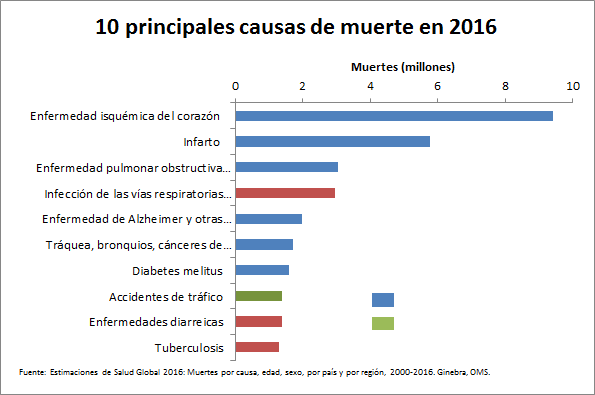
\includegraphics[width = .4\linewidth]{ figuras/Muertes2016.png}}
    \end{minipage}
            \begin{minipage}[b]{.5\linewidth}
        \centering
        \subcaptionbox{Fallecimientos en países con ingresos bajos-medios\label{subfig:Muertes2016Medio}}
            {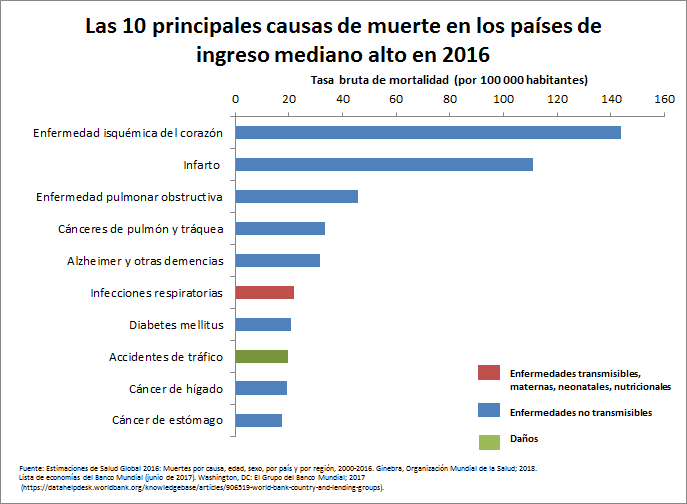
\includegraphics[width = .8\linewidth]{ figuras/Muertes2016MedioAlto.png}} 
    \end{minipage}
    \begin{minipage}[b]{.5\linewidth}
        \centering
        \subcaptionbox{Fallecimientos en países con ingresos altos\label{subfig:Muertes2016Alto}}
            {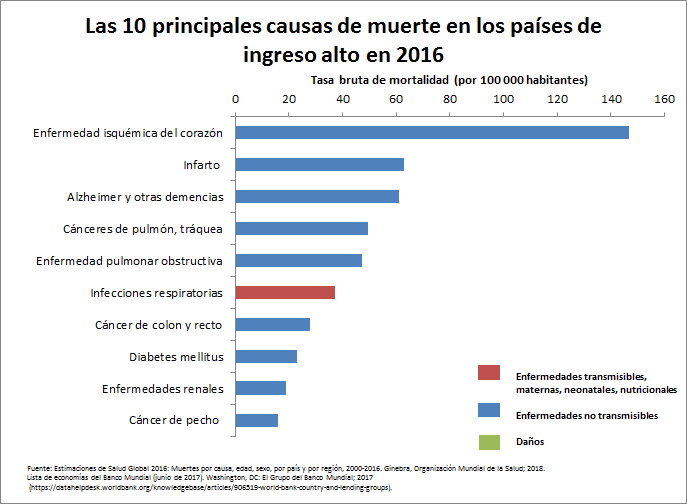
\includegraphics[width = .8\linewidth]{ figuras/Muertes2016Alto.png}}
        \end{minipage}
    \caption{Principales causas de muerte en 2016}
    \label{fig:Muertes2016}
\end{figure}

\subsection{Monitores portátiles de ECG}

Desde la década de los cuarenta se llevan investigando y mejorando dispositivos portátiles capaces de registrar las señales de ECG con el fin de obtener datos durante periodos extrahospitalarios. Concretamente el más antiguo de estos dispositivos es conocido como Holter, en honor a Norman J. Holter, quien desarrolló el primer prototipo en 1947, el cual pesaba alrededor de 38 Kg. No sería hasta el año 1962 cuando gracias a “Del Mar Engineering Laboratories” bajo el nombre de “Avionics Research Products Corporation” se consiguiera producir el primer dispositivo comercial, más ligero y capaz de almacenar el ECG de las últimas 24 horas. \cite{NormanHolter}

Desde sus inicios hasta hoy, el paradigma del registro de ECG portátil ha cambiado significativamente, gracias al desarrollo de la técnica, así como el uso de los monitores portátiles en la diagnosis y tratamiento de enfermedades cardiovasculares. En la actualidad hay dos tipos de dispositivos ampliamente utilizados, los ya mencionados monitores Holters y los monitores de eventos cardíacos. La principal diferencia entre ambos es la forma de almacenar los datos. Mientras que los holters registran los datos constantemente desde que el dispositivo es colocado por el médico hasta la consulta de vuelta, los monitores de eventos cardíacos son activados por los pacientes cuando padecen algún síntoma cardiovascular.

Teóricamente los monitores de eventos cardíacos son menos eficientes a la hora de la diagnosis de enfermedades que los Holters debido a que pierden los datos referentes a eventos que sean asintomáticos o que el paciente no percibe. Sin embargo encuentran su espacio en el mercado ya que típicamente son más pequeños y cómodos de usar que los Holters.

No obstante esto podría cambiar gracias al desarrollo de un nuevo tipo de monitores de eventos cardíacos, los supervisores de eventos cardíacos autodisparados. La teoría detrás de estos dispositivos es sencilla, si se puede analizar en tiempo real la señal ECG adquirida, entonces se puede detectar, en tiempo real y sin la intervención del paciente, el evento cardiaco anómalo. Y solo tras la detección, almacenar, e incluso trasmitir, el fragmento del ECG del paciente en el que se ha detectado el evento. Evitando así el enorme gasto de batería que conlleva la transmisión constante del registro y gozando de todas la ventajas de los supervisores cardíacos sin su mayor contra. La práctica, por otro lado, no es tan sencilla como se expondrá después.

La base del funcionamiento de un supervisor de eventos cardíaco autodisparados es la detección automática de los latidos presentes en la señal ECG.(TODO: Satija Reference) Localizados estos latidos, el supervisor debe extraer diversas características de ellos que permitan clasificarlos como anormales. La ocurrencia de estas anormalidades constituyen los eventos susceptibles de ser guardados o transmitidos.  Antes de continuar hablando de este tipo de monitores cardíacos es necesario comprender moderadamente los diferentes elementos de una señal ECG y qué datos médicos de interés se pueden obtener de ellos. 

\subsection{La señal ECG}

Como se puede ver en la figura~\ref{fig:ECGelements}, en la señal ECG correspondiente a un latido cardiaco, pueden apreciarse cinco elementos principales: la onda P, que representa la despolarización auricular, esto es, el latido de la aurícula; el complejo QRS, fruto de la despolarización ventricular, esto es, la contracción del ventrículo, y la onda T, que representa la repolarización ventricular, esto es, la relajación del ventrículo. Así, las ondas en sí mismas dan una idea de la actividad mecánica del corazón, y también se puede extraer mucha información de los intervalos entre las ondas, ya que reflejan las duraciones de los procesos biológicos del corazón.

%\begin{wrapfigure}{l}{0.5\linewidth}
\begin{figure}[ht]  
    \centering
        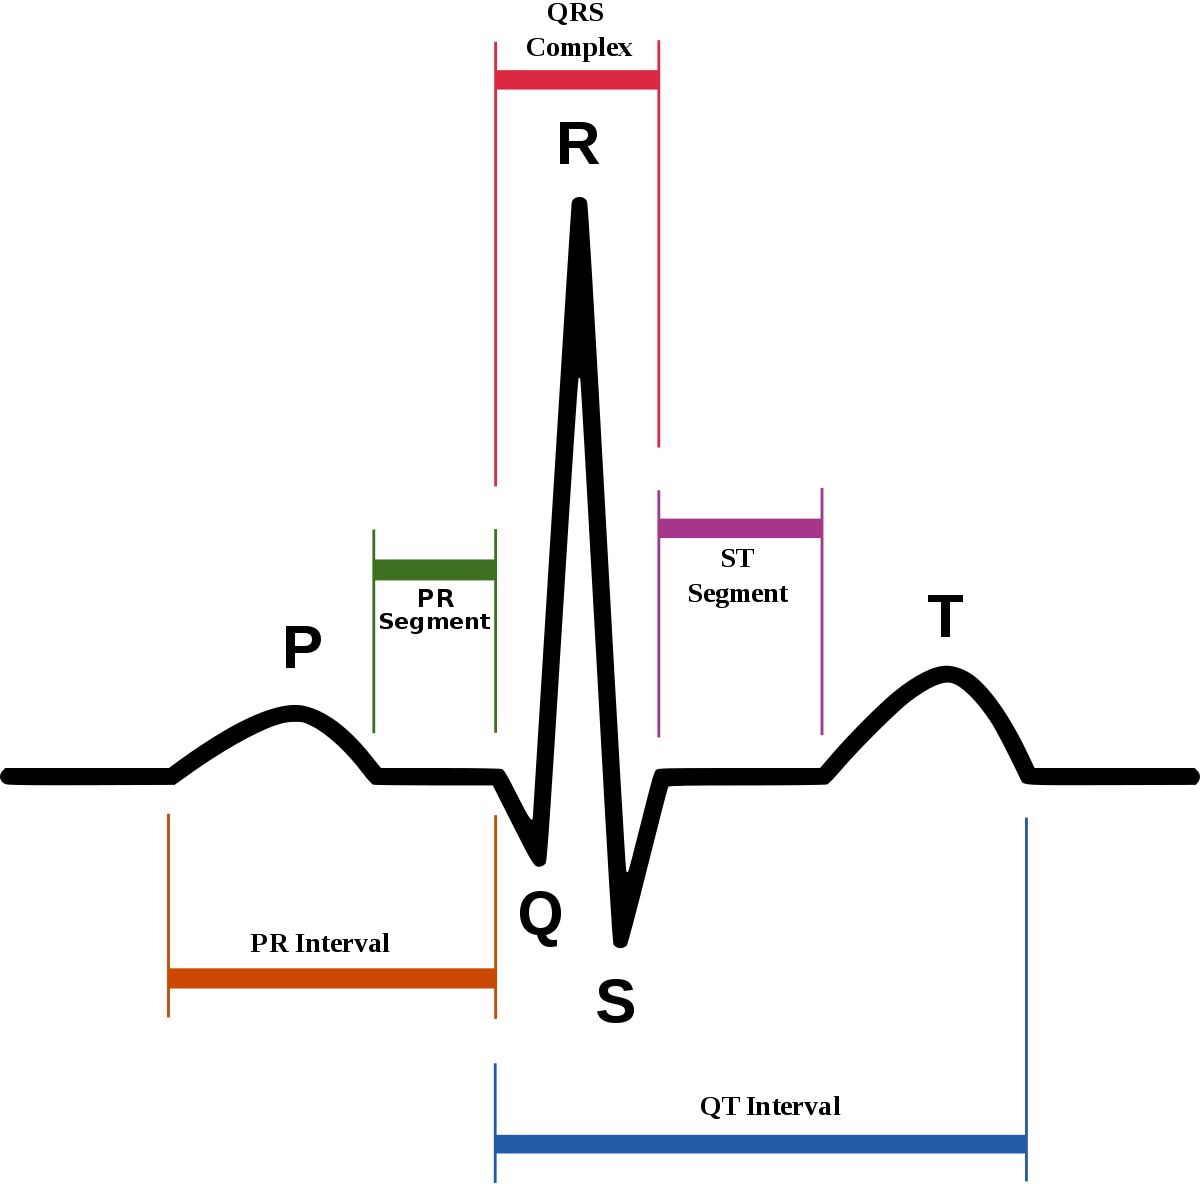
\includegraphics[width =0.4\linewidth]{figuras/ECGelementsDetailed.png}
    \caption{Elementos fundamentales ECG}
    \label{fig:ECGelements}
\end{figure}

En función de las posiciones donde se coloquen los electrodos a la hora de tomar las muestras, las señales se registrarán con una forma u otra. Estas posiciones se conocen como una derivaciones. En el ECG clásico estas derivaciones están estandarizadas en lo que se conoce como Sistema de doce derivaciones: un conjunto de seis derivaciones tomadas en las extremidades y otras seis, denominadas precordiales, que se sitúan en distintos puntos del torax. Las de las extremidades registran los potenciales que se transmiten al plano frontal y las precordiales recogen los potenciales del plano horizontal como puede verse en la figura \ref{fig:ECGelements}. \cite{Harrison}

Podría decirse que cada derivación hace las veces de un observador en un punto diferente, por lo que la señal resultante, que procede de diferencias potenciales con dirección y sentido, variará de polarización en según qué derivación, como puede “variar” el sentido de rotación de disco en función de si es observado desde arriba o desde abajo. LA FIGURA 1.2 EN CONCRETO CORRESPONDE A UN ECG DE UN SUJETO SANO TOMADO EN LA DERIVACIÓN II.

\begin{figure}[ht]
	\centering
		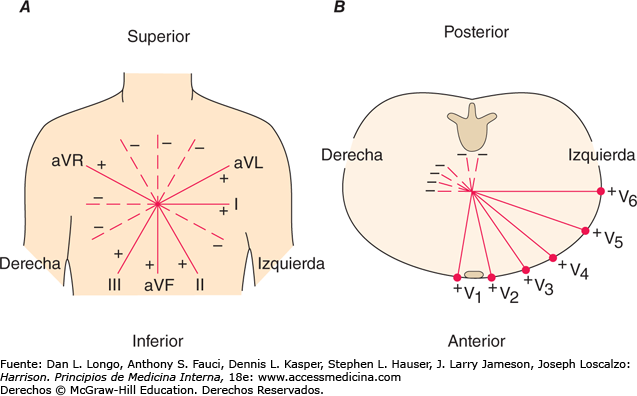
\includegraphics[width=0.9\linewidth]{figuras/derivations.png}
	\caption{Ilustración derivaciones ECG}
	\label{fig:derivaciones}
\end{figure} 

Desde que Willem Einthoven inventara el primer electrocardiograma hasta hoy la técnica ha mejorado enormemente y la precisión en las medidas hace posible observar fenómenos muy sutiles con un método de pruebas muy poco invasivo. La cantidad de patologías que pueden diagnosticarse realizando un electrocardiograma en el momento apropiado es enorme. \cite{PatologiasECG} Por ejemplificar esto, diremos que tan solo mediante la morfología de la onda P se pueden diagnosticar más de 15 patologías diferentes, por ejemplo, una fibrilación auricular cuando se hay una ausencia total de la onda o varios tipos de taquicardia, cuando se observan ausencias parciales. También se puede detectar un crecimiento auricular anormal si se observa que la onda es bifásica. Y un largo etcétera de patologías.

En muchas ocasiones la detección de estas patologías requiere como paso previo la detección del propio latido cardíaco. Una vez detectado se pueden realizar procesados complicados basados en la morfología de la onda u otros más sencillos como el cálculo de la tasa cardíaca, que pueden aportar mucha información.

\subsection{Detectores de QRS: cálculo de la tasa cardíaca basada en ECG}

Una vez reconocidos los latidos cardíacos se puede medir la diferencia de tiempo entre dos latidos, esto se conoce como intervalo RR (Ver figura~\ref{fig:RRInterval})  de donde se obtiene la frecuencia cardíaca instantánea, parámetro típico que es empleado para activar numerosos supervisores de eventos cardíacos autodisparados. Este proyecto se centra en este parámetro y, en particular, en los algoritmos de detección de latidos que posibilitan su obtención.  

\begin{figure}[ht]
	\centering
		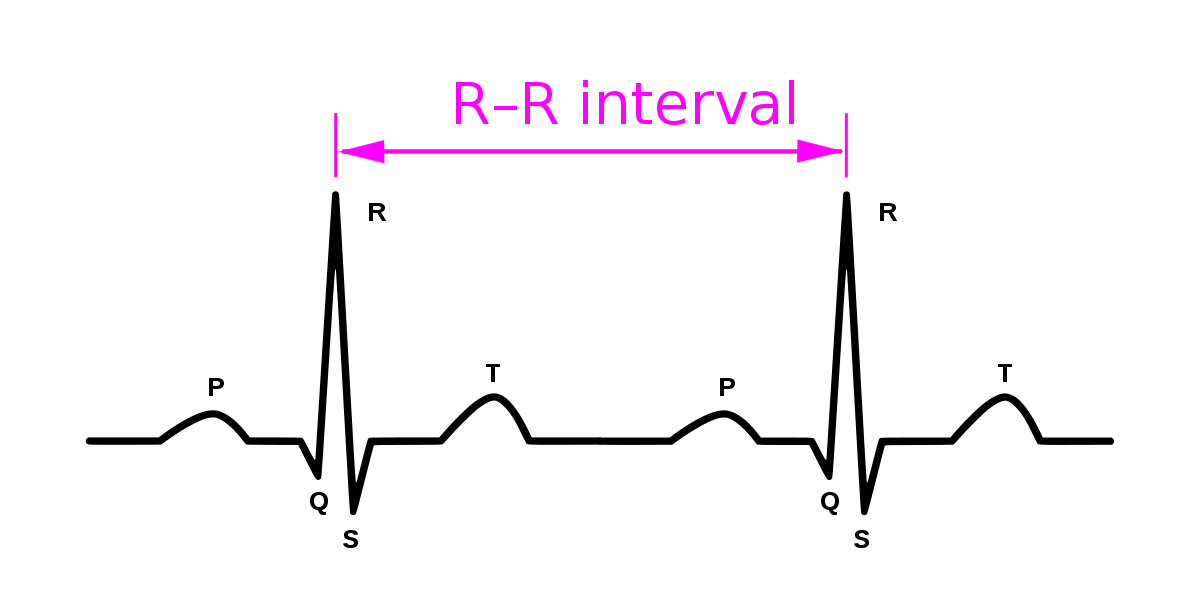
\includegraphics[width=0.6\linewidth]{figuras/RRInterval.png}
	\caption{Representación intervalo R-R}
	\label{fig:RRInterval}
\end{figure} 

\clearpage
En la literatura actual existen numerosos algoritmos muy testeados y eficaces a la hora de detectar el complejo QRS y ,en base a esa detección, calcular la tasa cardíaca. Tradicionalmente se ha desarrollado para ser ejecutados sobre unos datos extraídos previamente y almacenados en memoria. Pero esto no sirve para ser aplicados en tiempo real por diseño, así que en los últimos años se ha estado invirtiendo mucho esfuerzo en desarrollar algoritmos de tiempo real. Siendo el más conocido y uno de los más antiguos el de “Pan Tompkins” basado en el análisis de la pendiente, la intensidad y la duración de los complejos QRS.\cite{PanTompkins} A día de hoy se pueden encontrar numerosos estudios sobre nuevas metodologías para llevar a cabo esta tarea como algoritmos especializados en muestras con mucho ruido\cite{RsSlope} o métodos con diferentes aproximaciones como máquinas de estado finitas\cite{FSM} o empleando coeficientes de wavelet.\cite{Wavelet}

Sin embargo no resulta sencillo encontrar la forma de testar dichos métodos en entornos reales. Para realizar las pruebas pertinentes se hace uso de bases de datos estandarizadas como la MIT-BIH (TODO: Poner esto good con referencia y toh.), evaluando principalmente la tasa de falsos positivos y negativos. (TODO: Referencia Pootja 2017) Un ejemplo de algoritmo para determinar la fiabilidad de un algoritmo se puede encontrar en la norma para marcado CE de los Holter de ECG (TODO: referencia- AENOR, te la mando por correo)

Por otro lado, la tendencia actual es emplear dispositivos cada vez de menor consumo que suelen ir acompañados de menores recursos y baterías más pequeñas. Por ello cada vez se requieren métodos de detección con menor complejidad computacional pero con una robustez suficiente para ser caracterizados como fiables. Minimizando así las transmisiones de datos a lo estrictamente necesario, ahorrando batería para poder tomar medidas durante un periodo más largo. En este contexto resulta complejo evaluar cuando un algoritmo es suficientemente válido o no debido únicamente a su fiabilidad de detección, influyen también parámetros como el consumo de batería en ejecución, la necesidad de memora y la portabilidad de este a lenguajes de bajo nivel.

\subsection{Breves conclusiones}

Como se ha mencionado anteriormente las patologías cardíacas son una de las mayores causas de mortalidad en todo el mundo, por ende los supervisores de eventos cardiacos autodisparados podrían tener un efecto directo en la detección y seguimiento de estas patologías. La base principal de estos supervisores radica en la correcta detección de los complejos QRS, no solo de una forma fiable y en tiempo real, sino también con un consumo mínimo de recursos los recursos hardware del sistema.

\section{Objetivo}
%\label{sec:intro:obj}
%En esta sección, se describe el \miindex{objetivo del proyecto}, es decir, qué pretende, a qué aspira, cuál es su meta. Es importante comprender esta sección, porque de otro modo, no se entiende el resto de la documentación.
El objetivo de este proyecto es el diseño y la implementación de un entorno de pruebas genérico para testear diferente algoritmos de medida de tasa cardíaca instantánea basados en ECG en un entorno portátil de tiempo real con recursos limitados. Este entorno de pruebas será validado con un ejemplo concreto de algoritmo aplicado sobre señales ECG tomadas de la MIT-BIH.

Como objetivos personales de este proyecto se propusieron la profundización en los conocimientos sobre el procesado de datos, concretamente los datos de electrocardiogramas. Además se propuso emplear dicho proyecto para investigar y aprender a realizar documentación con \LaTeX
%\section{Metodología y directrices seguidas}


\section{Estructura del documento}
TODO: En esta sección, se explican los posteriores capítulos u otra información adicional que el proyecto contenga.

\chapterend


%\part{Desarrollo del proyecto}

% Capítulo 02.
%%%%%%%%%%%%%%%%%%%%%%%%%%%%%%%%%%%%%%%%%%%%%%%%%%%%%%%%%%%%%%%%%%%%
%%% Documento LaTeX 																						%%%
%%%%%%%%%%%%%%%%%%%%%%%%%%%%%%%%%%%%%%%%%%%%%%%%%%%%%%%%%%%%%%%%%%%
% Título:		Capítulo 1
% Autor:  	Ignacio Moreno Doblas
% Fecha:  	2014-02-01, actualizado 2019-11-11
% Versión:	0.5.0
%%%%%%%%%%%%%%%%%%%%%%%%%%%%%%%%%%%%%%%%%%%%%%%%%%%%%%%%%%%%%%%%%%%
% !TEX root = A0.MiTFG.tex
\chapterbegin{Manual básico de \LaTeX}
\label{chp:ManLaTeX}
\minitoc

\begin{sinopsis}
\label{sec:chpltx:sinop}
Éste es el primer capítulo de desarrollo del proyecto, definido y estructurado según el autor necesite y desee. En este caso, no hay guías genéricas para cualquier proyecto más allá del manual de estilo disponible en~\cite{GuiaEstilo}~\footnote{\url{https://www.uma.es/media/tinyimages/file/Manual_de_estilo_ETSIT_TFG_TFM_PFC.pdf}}.

En esta plantilla, este capítulo se enfoca como un manual básico de \LaTeX\ para cualquiera que lo necesite. Como plantilla, está basada en la \ttw{\textbackslash documentclass} tipo \ttw{book}, empleando partes, capítulos, secciones, etc. \LaTeX\ es una herramienta muy orientada a documentos que contienen tablas, figuras, referencias cruzadas, bibliografía, glosarios, apéndices, ecuaciones matemáticas o unidades físicas.
\end{sinopsis}

\section{Estructura y formato del proyecto}
\label{sec:EstrForm}
Esta plantilla sigue las especificaciones de la ETSIT para presentar un TFG/TFM. Igualmente, la plantilla con su material adicional está disponible en la \tit{web} del centro (\url{www.etsit.uma.es}.)

\section{Apartados de la plantilla}

La plantilla está estructurada en los siguientes archivos y directorios:

\begin{itemize}
	\item{Veintitrés ficheros \TeX\ (extensión \ttw{.tex}).}

	\item{Un fichero Bib\TeX\ (extensión \ttw{.bib}).}

	\item{Un fichero PDF resultante.}

	\item{Dos ficheros \TeX nicCenter (extensión \ttw{.tps} y \ttw{.tcp}) por si quieres utilizar este entorno (aunque ha quedado un poco anticuado).}

	\item{Dos directorios complementarios.
		Uno de código fuente (\ttw{code}) y otro de gráficos (\ttw{figuras}).}

\end{itemize}

Existen varias alternativas para trabajar con documentos \LaTeX, como \TeX maker, \TeX studio, o con cualquier editor de texto y el entorno de compilación de \LaTeX\ (MiKTeX --Windows--, LiveTeX --Linux--, MacTeX, --MacOS--). Otra alternativa muy popular es  Overleaf (\url{www.overleaf.com}) que permite la edición on-line y colaborativa con otros usuarios.

\begin{figure}[ht]
	\centering
		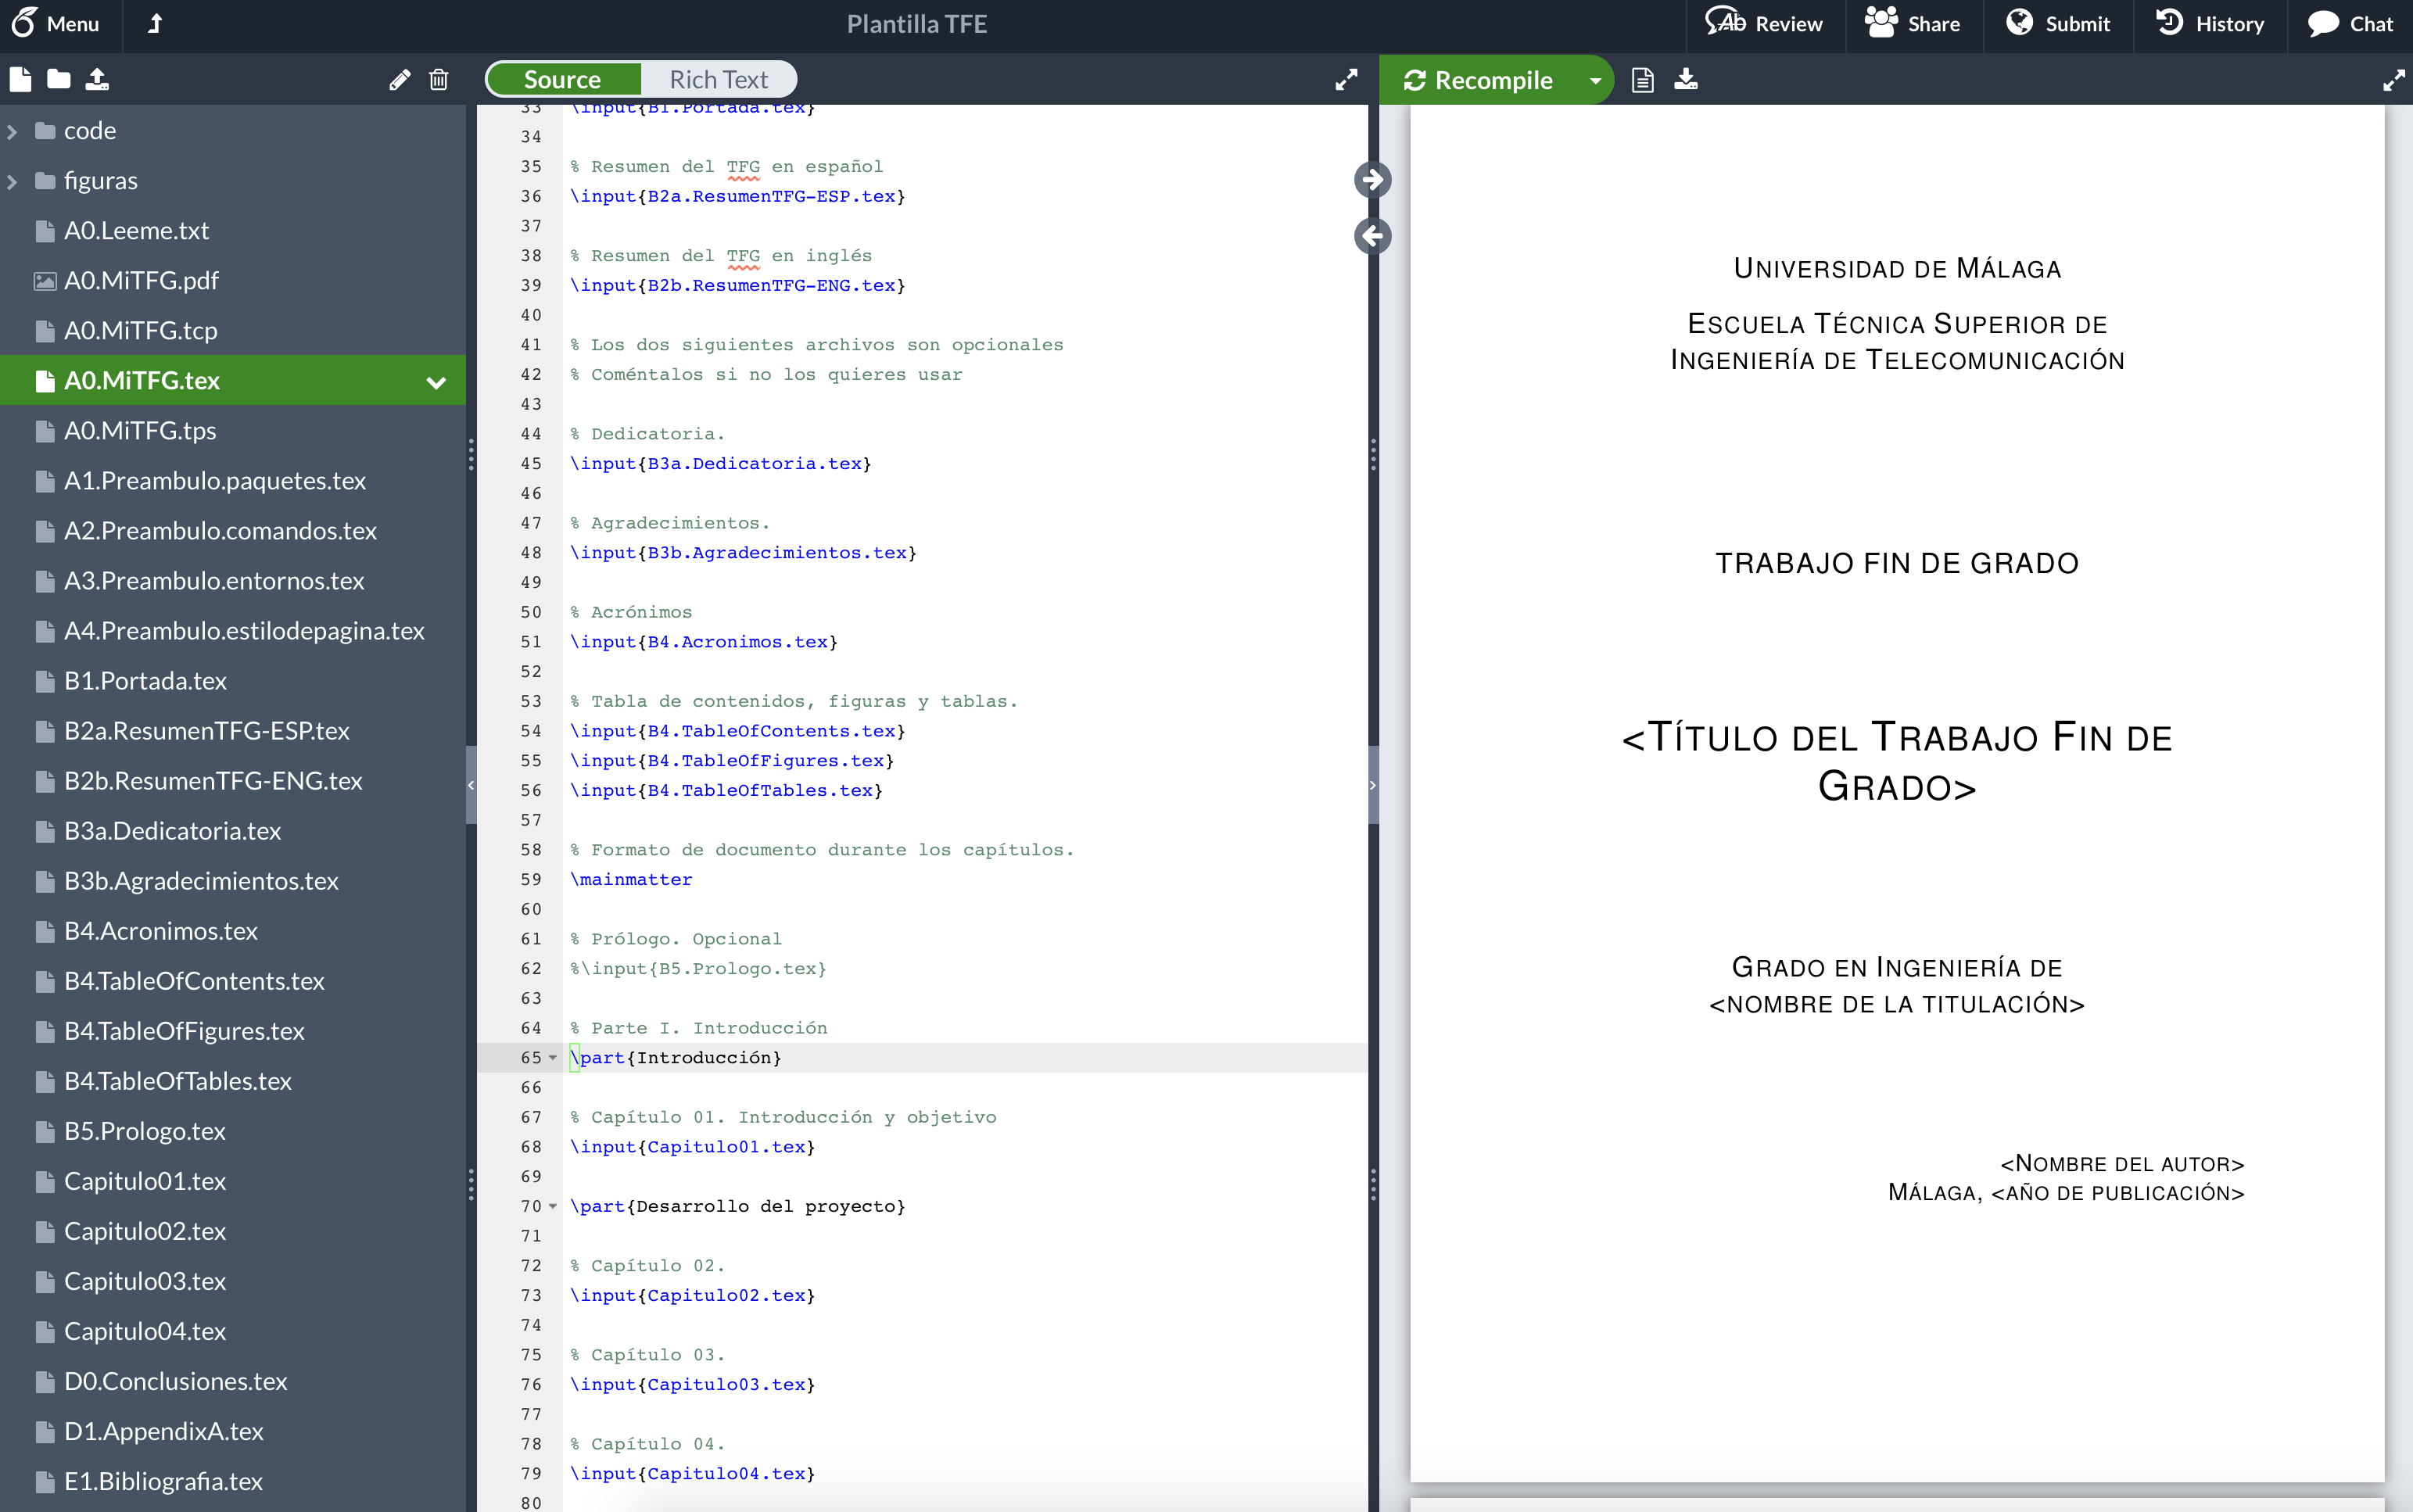
\includegraphics[width=\linewidth]{figuras/overleaf.png}
	\caption{Ficheros de la plantilla y aspecto de Overleaf}
	\label{fig:ficherosPlan}
\end{figure}

En la figura~\ref{fig:ficherosPlan}, puede verse la lista de ficheros del proyecto, tal y como se presenta en el entorno Overleaf. A su vez, entre los veintitrés ficheros \TeX\ encontramos un documento maestro (\ttw{A0.MiTFG.tex}) a partir del cual se referencia el resto de archivos, los cuales se reparten en cuatro clases.

Los archivos contienen un prefijo que hace que su posición en la lista sea equivalente al orden en el documento PDF resultante. Este prefijo es una letra y un número en arábigo. Por ejemplo, el documento maestro, ``\ttw{A0.MiTFG.tex}'', comienza por \ttw{A0} para que figure en primer lugar.

Las cuatro clases de archivos antes mencionadas son las siguientes:

\begin{descript}
	\item[Archivos de preámbulo] Forman el preámbulo del documento \LaTeX\ y su contenido no se visualiza en el fichero PDF resultante. Comienzan por la letra \ttw{A}
	\item[Archivos iniciales] Son los archivos iniciales del proyecto, desde la portada, dedicatoria, acrónimos, tablas de contenido y prólogo. Comienzan por la letra \ttw{B}.
	\item[Archivos de capítulo] Son los ficheros de capítulo del proyecto. Dado que su primera letra coincide con la letra C, no tienen ninguna identificación especial.
	\item[Archivos finales] Por último, los archivos de conclusiones, apéndices, bibliografía y glosario (\tit{index} en inglés).
\end{descript}

En la figura~\ref{fig:ficherosPlan}, segmentada en tres paneles, se observa en la parte izquierda todos estos archivos ordenados según el orden secuencial. Esta ordenación permite una elaboración cómoda del proyecto por lo que se recomienda mantener esta organización. En el panel central se muestra parte del contenido del fichero \LaTeX\ principal y en el panel derecho el fichero PDF al que da lugar después de la compilación.

En el documento PDF resultante, el proyecto se estructura en los nueve apartados siguientes:
\begin{descript}
	\item[Portada y encuadernación.] Es específica de cada tipo de trabajo (TFG/TFM) y debe ajustarse a lo establecido en la Secretaría.

	\item[Primeras páginas.] Contendrá las páginas que correspondan con el tipo de trabajo y que son específicas de cada tipo de proyecto. En el TFG/TFM de la ETSIT estas primeras páginas contienen el título, autor, tutor, resumen y otra identificación del trabajo, tanto en español como en inglés.

	\item[Dedicatoria y agradecimientos.] La sección de agradecimientos (evidentemente, no obligatoria) define un apartado donde el estudiante puede (y quizás, debe) referenciar a aquellas personas y/o instituciones que, de manera generosa, han colaborado de algún modo en la gestación y desarrollo del PFC. Igualmente el estudiante también puede utilizar este apartado libremente para mencionar a aquellos familiares, compañeros, amigos, etc., de los que ha recibido apoyo personal, moral o afectivo. Por contra, no debe utilizarse esta sección para expresar opiniones críticas, ácidas o mordaces contra particulares o instituciones de la ETSIT o la Universidad debido a correcciones, exámenes, trato recibido u otras interacciones o causas cualesquiera que sean, ya que esto estaría fuera del ámbito del proyecto.


	\item[Índice.] En la plantilla, se genera un índice, índice de figuras e índice de tablas, numerado automáticamente con su correspondiente página. Ésta es una de las ventajas de \LaTeX.

	\item[Capítulo 1. Introducción.] En éste se hará una introducción al ámbito del trabajo, comenzando por el contexto general y aproximándose progresivamente a los aspectos más concretos que se traten.	Es conveniente terminar con una exposición clara de los objetivos que se persiguen, la metodología empleada y el contenido del proyecto.

	\item[Capítulos de desarrollo.] A continuación el desarrollo de los distintos capítulos o epígrafes que componen el trabajo. En esta plantilla, éste es el primero de esos capítulos, que además incluye un manual de \LaTeX\ práctico.

	\item[Conclusiones.] En este apartado el estudiante expondrá con claridad los resultados o conclusiones obtenidas y el juicio crítico que le merecen.

	\item[Referencias bibliográficas.] A continuación de las conclusiones se insertará un apartado con todas las referencias bibliográficas que aparezcan en la memoria: revistas, artículos de revistas o congresos, páginas web, etc. En \LaTeX, existe el entorno Bib\TeX\ para almacenar y referenciar bibliografía.

	\item[Apéndices.] Finalmente se presentarán los apéndices, si los hubiere. En esta plantilla se provee del entorno \ttw{\textbackslash appendix} para crearlos.
\end{descript}

Por último, respecto de las secciones del proyecto, hay que tener en cuenta que un proyecto puede ser un documento extenso, complejo y por eso se recomienda seguir este tipo de reglas para facilitar su elaboración. Además, se recomienda generarlo incrementalmente, anulando las secciones que no se utilicen desde el documento maestro. Por ejemplo, al elaborar el capítulo tres y generar el documento PDF, no es necesario ni el prólogo, ni los capítulos anteriores ni posteriores, por tanto, pueden comentarse con el símbolo tanto por ciento (\ttw{\%}) en el documento maestro (A0.MiTFG.tex). En ese caso, la compilación será más rápida, el PDF más breve y la revisión también.

\section{Referencias Cruzadas}
\label{sec:RefCruz}

Normalmente, surge la necesidad de referenciar información desde una sección de la documentación hasta otra. Esta información referenciada puede ser un apartado, una figura, una tabla, una página o una ecuación.

Por ejemplo, el presente capítulo~\ref{chp:ManLaTeX} comienza en la página~\pageref{chp:ManLaTeX} y está titulado \nameref{chp:ManLaTeX} (para generar estas tres referencias en el documento se han usado los comandos \LaTeX\  \verb|\ref{chp:ManLaTeX}|, \verb|\pageref{chp:ManLaTeX}| y \verb|\nameref{chp:ManLaTeX}|, respectivamente, ya que el \verb|\chapter| está etiquetado con \verb|\label{chp:ManLaTeX}|). Es decir, tanto el número de capítulo, su página o su título no están escritos manualmente, sino referenciados mediante etiquetas.

Las referencias cruzadas se realizan siguiendo los siguientes pasos:

\begin{enumerate}

	\item Se etiqueta el elemento a referenciar, ya sea sección, apartado, figura, tabla, ecuación o cualquier otro con el comando \verb|\label{}|. Para ello, se escribe próximo a él un identificador con el comando \verb|\label{}|. Por ejemplo, \verb|\label{sec:RefCruz}| es la etiqueta del presente apartado. Se recomienda, en general, usar como prefijo \ttw{chp} para capítulos, \ttw{sec} para secciones, \ttw{eq} para ecuaciones, \ttw{fig} para figuras o \ttw{tab} para tablas. También usar los dos puntos (:) como separador entre el prefijo y el resto de la etiqueta. A lo largo de esta plantilla pueden encontrarse muchas etiquetas de ejemplo.

	\item Se compila si es la primera vez que se crea la etiqueta. Aunque este paso depende del compilador, en el caso de MiK\TeX\ es necesario compilar para indexar la etiqueta y poder referenciarla, como se indica en el paso siguiente.

	\item Se referencia una etiqueta ya definida con el comando \verb|\ref{}|. Por ejemplo, \verb|\ref{sec:RefCruz}| referencia el presente apartado, cuyo valor es \ref{sec:RefCruz}.

	\item Se compila el documento para crear la referencia a partir de los índices generados en la compilación anterior. Esto es especialmente importante, porque la referencia se crea a partir de la compilación anterior. Si el apartado cambia de página, se debe re-compilar para actualizar la referencia; si no se compila, la referencia se hará según la información desactualizada, es decir, a la página anterior. \emph{En general y términos prácticos, se debe compilar frecuentemente para tener siempre información actualizada.}

\end{enumerate}

Muchos de los entornos para compilar \LaTeX\ son capaces de compilar repetidas veces de forma automática hasta que se resuelven las referencias cruzadas. Entre ellos encontramos Overleaf o Atom con el paquete LaTeX, pero también se puede conseguir el mismo efecto compilando desde una consola usando el comando ``\texttt{make}'' o el comando ``\texttt{latexmk -pdf A0.MiTFG.tex}''.

%\section{Formato de otros elementos}
\section{Figuras}

Las figuras aparecerán centradas y se verán siempre acompañadas por un título explicativo, también centrado y situado en la parte inferior. El título comienza por la palabra ``Figura'' con un identificador de figura formado por el número de capítulo y el número de figura. El propio título debe ser lo bastante explicativo para poder entender el significado de la figura o distinguirla de las demás, pero no debe ser demasiado extenso ya que dificultaría la legibilidad. Para cualquier explicación o justificación más extensa, se debe describir en un párrafo aparte, utilizando referencias cruzadas. Además, tanto el título como el identificador aparecerán referenciados en el índice de figuras al principio de la memoria (esto último ya se consigue de forma automática al compilar).


	En \LaTeX, el entorno \ttw{figure} automatiza la presentación de figuras siguiendo estas reglas. A continuación se ve el texto original utilizado para la figura~\ref{fig:marcaETSIT} de la página~\pageref{fig:marcaETSIT}, titulada \nameref{fig:marcaETSIT}.
	Para respetar los espacios y el texto original se ha utilizado el entorno \ttw{lstlisting}.

\lstset{
  language=[LaTeX]TeX, framexleftmargin=0mm, frame=shadowbox,
  rulesepcolor=\color{gray}, numberstyle=\tiny,
  keywordstyle=\color{blue}\bfseries
}

\begin{lstlisting}[numbers=left,morekeywords={includegraphics}]
\begin{figure}[ht]
	\centering
	
\includegraphics[width=3cm]{figuras/MarcaETSIT.pdf}
	\caption{Marca Teleco de la ETSIT en la UMA}
	\label{fig:marcaETSIT}
\end{figure}
\end{lstlisting}

\begin{figure}[ht]
	\centering
		
\includegraphics[width=9cm]{figuras/MarcaETSIT.pdf}
	\caption{Marca Teleco de la ETSIT en la UMA}
	\label{fig:marcaETSIT}
\end{figure}

Puede ser necesario presentar una figura conteniendo varias en su interior. En ese caso, el entorno \verb|\minipage| puede cumplir esta función aunque se recomienda como mejor alternativa el uso del paquete \texttt{subcaption}. En la figura~\ref{fig:marca:UMA}, se muestran los dos marcas de la Universidad de Málaga usando el entorno \verb|\minipage|.

	\begin{figure}[ht]
		\centering
			\begin{minipage}[l]{6cm}
			\includegraphics[width=6cm]{figuras/MarcaUMA.pdf}
			\end{minipage}
			\ \
			\begin{minipage}[r]{6cm}
			
\includegraphics[width=6cm]{figuras/marcaumaes.pdf}
			\end{minipage}
		\caption{Marcas oficiales de la UMA}
		\label{fig:marca:UMA}
	\end{figure}

La alternativa que ofrece el paquete \texttt{subcaption} permite la utilización del entorno \verb|\subfigure| y ofrece mayor funcionalidad como vemos en la Figura~\ref{fig:marcaUMA}. Cada ``subfigura'' puede tener su propio \texttt{caption}, el cual se puede referenciar como Figura~\ref{fig:marcaUMA-a} y Figura~\ref{fig:marcaUMA-b}.

	\begin{figure}[ht]
	  \centering
	  \begin{subfigure}[t]{0.4\linewidth}
	    \centering
	    \includegraphics[width=\textwidth]{figuras/MarcaUMA.pdf}
			\caption{Marca UMA.}
	    \label{fig:marcaUMA-a}
	  \end{subfigure}%
		\hfill
	  \begin{subfigure}[t]{0.4\linewidth}
	    \centering
	    
\includegraphics[width=\textwidth]{figuras/marcaumaes.pdf}
	    \caption{Marca uma.es.}
	    \label{fig:marcaUMA-b}
	  \end{subfigure}
	  \caption{Las dos marcas de la UMA.}
	  \label{fig:marcaUMA}
	\end{figure}

También es importante conocer algunas características sobre los gráficos vectoriales y de tipo bitmap (también llamados rasterizados\footnote{en inglés, \tit{raster}.}) y sobre los formatos aceptados por \LaTeX\ para gráficos. En general, hay dos tipos de ficheros gráficos en un ordenador:

\begin{descript}
	\item[Bitmap o rasterizados] El gráfico está formado por una matriz de píxeles, como en una fotografía digital.
	Ejemplos de formatos bitmap son JPG, PNG, GIF o TIFF.

	\item[Vectoriales] El gráfico está formado por curvas geométricas, lo que hace que independientemente de la escala mostrada, se mantenga la misma definición, tanto en color como en forma.
	Ejemplos de formatos vectoriales son EPS (\tit{Encapsulated PostScript}), PDF o SVG (\tit{Scalable Vector Graphics}).
	Un ejemplo concreto es la figura~\ref{fig:marcaETSIT}, que está en PDF.
\end{descript}

	Si se desea insertar un gráfico vectorial y se emplea el compilador \ttw{pdflatex} o el comando \texttt{latexmk -pdf}, el formato del gráfico debe ser PDF.
	Si los gráficos vectoriales están en otro formato, tales como SVG o EPS, es necesario usar un conversor.
	Una opción sencilla y gratuita es el editor Inkscape\R, disponible en Internet. No es necesario instalarlo, ya que puede encontrarse una edición portable, que sólo requiere ser descomprimida y ejecutada.

\section{Tablas}
	La presentación de las tablas es equivalente a la de las figuras, tanto en su posición centrada como en su título. En \LaTeX\ existen varios entornos para presentar una tabla, dependiendo de qué se desee:

	\begin{ite}
		\item El entorno \tbf{\ttw{tabular}} permite crear una tabla a partir de definir sus filas, columnas y su formato.
		Está limitado a no poder fragmentarse en varias páginas si la tabla es demasiado extensa.

		\item El entorno \tbf{\ttw{table}} formatea una tabla, una sección de código fuente o algún componente equivalente.
		Permite posicionar, ponerle un título y añadirlo al índice de tablas. En el ejemplo siguiente, se utilizan los dos entornos, uno \ttw{table} y otro \ttw{tabular} anidado en el primero.

		\item El entorno \tbf{\ttw{longtable}} es equivalente a \ttw{tabular}, pero además supera la limitación de extender una tabla a más de una página.
	\end{ite}

	De nuevo, las tablas aparecen referenciadas en un índice de tablas tras el índice temático y del índice de figuras.

	A continuación, se muestra el código \LaTeX\ de la tabla~\ref{tab:SAR}, presente en la página~\pageref{tab:SAR}, titulada \nameref{tab:SAR}.

\begin{lstlisting}
\begin{table}[ht]
\centering
\begin{tabular}{|c|p{14ex}|c|c|}
	\hline \hline
	\tbf{Requisito} & \tbf{Plat. Referencia} &
		\tbf{SAR (dBm)} & \tbf{Tol.}\\ \hline
	R101  &  Baytrail 		& 5 & 1 \\ \hline
	R201  &  Clovertrail 	& 6 & 2 \\ \hline
	R301  &  Merrifield 	& 4 & 3 \\ \hline \hline
\end{tabular}
\caption{Tabla de SAR por Plat. de Referencia}
\label{tab:SAR}
\end{table}
\end{lstlisting}

	%\begin{center}
	\begin{table}[ht]%
	\centering
	%\begin{longtable}{c|p{10cm}}
	\begin{tabular}{|c|p{14ex}|c|c|}
		\hline \hline
		\tbf{Requisito} & \tbf{Plat. Referencia} &
			\tbf{SAR (dBm)} & \tbf{Tol.}\\ \hline
		R101  &  Baytrail 		& 5 & 1 \\ \hline
		R201  &  Clovertrail 	& 6 & 2 \\ \hline
		R301  &  Merrifield 	& 4 & 3 \\ \hline \hline
	\end{tabular}
	\caption{Tabla de SAR por Plat. de Referencia}
	\label{tab:SAR}
	\end{table}
	%\end{longtable}
	%\end{center}%\end{table}

\section{Código fuente}

En un proyecto de desarrollo, es común introducir extractos de código en diferentes lenguajes como C, C++, Matlab, Python, Java, bash script, etc. En estos casos, los entornos de \LaTeX\ disponibles por defecto no permiten mostrar esta información.

El paquete \ttw{listings} es muy utilizado para presentar código fuente, respetando las tabulaciones para que la lectura sea confortable. En esta plantilla, en la sección de paquetes (fichero \texttt{A1.Preambulo.paquetes.tex}) se ha configurado el paquete \texttt{listings} para que use el lenguaje Python a la hora de presentar código con resaltado de sintaxis (\emph{syntax highlighting}). 

Este paquete es fácilmente adaptable para otros lenguajes y de hecho, en los listados \LaTeX\ con los ejemplos de uso del entorno \texttt{figure} y \texttt{table} mostrados previamente, se ha configurado \texttt{listings} para que resalte la sintaxis de código \LaTeX.

En la sección de comandos, se ha definido el comando \ttw{code}, el cual permite crear una sección de código siempre que indiquemos los tres argumentos entre llaves:
\begin{itemize}
    \item título a mostrar
    \item fichero fuente correspondiente
    \item etiqueta con la que se harán referencias a dicho Listado
\end{itemize}

Por ejemplo, mediante el comando: 

\begin{verbatim}
	\code{Ejemplo de código Python}{code/pythonCode.py}{code:python}
\end{verbatim}

\noindent conseguimos el Listado~\ref{code:python}.

\lstset{
  language=Python, %Puede ser C, C++, Java, etc.
  showstringspaces=false,
  formfeed=\newpage,
  tabsize=4,
  commentstyle=\itshape,
  morekeywords={models, lambda, forms}
}

\code{Ejemplo de código Python}{code/pythonCode.py}{code:python}

El paquete \texttt{listings} es muy completo y configurable\footnote{Ver \url{http://texdoc.net/texmf-dist/doc/latex/listings/listings.pdf} si quieres ver todas las opciones y sacarle el máximo jugo.}. Por ejemplo, con el siguiente código \LaTeX:

\begin{verbatim}
\begin{minipage}{0.96\linewidth}
  \begin{center}
    \begin{lstlisting}[language={[11]C++}, frame=lines, numbers=left,
        numberstyle= \tiny,	keywordstyle=\color{blue}\bfseries,
        framexleftmargin = 5mm,
        caption={Hola mundo en C++},
        label={code:holaC++}]
#include <iostream>
int main(){
  std::cout << "Hola mundo\n";(@\label{lst:cout}@)
  return 0;
}
    \end{lstlisting}
  \end{center}
\end{minipage}
\end{verbatim}

\noindent obtenemos el Listado \ref{code:holaC++}, donde hemos insertado una \texttt{label} que se procesa en \LaTeX\ gracias a los comandos de escape \texttt{(@} y \texttt{@)}, y por tanto podemos hacer referencia a la línea del Listado que queramos explicar. Por ejemplo, la línea~\ref{lst:cout} del Listado~\ref{code:holaC++} provoca que se imprima la cadena ``Hola mundo'' cuando se ejecuta el programa.

\begin{minipage}{0.96\linewidth}
\begin{center}
    \begin{lstlisting}[
        language   = {[11]C++},
        frame      = lines,
	    numbers		 = left,
		numberstyle= \tiny,
		keywordstyle=\color{blue}\bfseries,
		framexleftmargin = 5mm,
        caption    = {Hola mundo en C++},
        label      = {code:holaC++}
    ]
#include <iostream>
int main(){
  std::cout << "Hola mundo\n";(@\label{lst:cout}@)
  return 0;
}
\end{lstlisting}
\end{center}
\end{minipage}

\section{Símbolos matemáticos y físicos}
Los proyectos de ingeniería suelen presentar símbolos matemáticos y físicos, tanto en los párrafos como en tablas, figuras y ecuaciones. Existen reglas para la notación, formateo y estilo de elementos matemáticos, tales como utilizar un símbolo por variable (p.ej., $x$ e $y$, pero no $xx$ o $yy$), escribir los símbolos en cursiva y las magnitudes y unidades físicas en redonda o el espaciado entre variables.

\LaTeX\ está construido sobre \TeX, que fue concebido originalmente para escribir textos matemáticos con alta calidad, de forma que funciona perfectamente en estos entornos. Su integración es suave, rápida y sencilla de seguir, una vez se tiene algo de práctica.
Esta facilidad se hace extensiva al uso de magnitudes físicas con sus correspondientes múltiplos. \LaTeX\ ofrece el paquete \ttw{SIunits}, ya incluído en esta plantilla.

A continuación se muestran varios ejemplos de su uso, con su código original. Para ecuaciones integradas en el párrafo, tan sólo se usa el símbolo dólar (\$) antes y después del símbolo. Por ejemplo, con \verb|$x$| se indica la variable $x$. Las ecuaciones en línea deben usarse para expresiones cortas y que no requieran de mucho espacio vertical. Para escribir ecuaciones más largas están los entornos \ttw{displaymath}, \ttw{equation} y \ttw{align}.

Los entornos \ttw{displaymath} y \ttw{equation} muestran una ecuación en una línea. La diferencia entre ambos es que el primero no realiza una numeración de la ecuación y el segundo sí. Sólo se pueden referenciar las ecuaciones numeradas.

Por ejemplo, la ecuación de la proporción áurea en entorno \ttw{displaymath},

\lstset{language=[LaTeX]TeX,
keywordstyle=\color{blue}\bfseries
}
\begin{lstlisting}
	\begin{displaymath}
		\phi^2 - \phi - 1 = 0
	\end{displaymath}
\end{lstlisting}

\begin{displaymath}
	\phi^2 - \phi - 1 = 0
\end{displaymath}

\noindent mientras que si usamos el entorno \ttw{equation}, mostraremos la ecuación~\ref{eq:aurea} en la página~\pageref{eq:aurea}:
\begin{lstlisting}
	\begin{equation}
		\phi^2 - \phi - 1 = 0
		\label{eq:aurea}
	\end{equation}
\end{lstlisting}

\begin{equation}
	\phi^2 - \phi - 1 = 0
	\label{eq:aurea}
\end{equation}

%\begin{equation}
	%\int_0^\infty \mathrm{e}^{-x}\,\mathrm{d}x = z
	%\label{eq:prueba}
%\end{equation}

En caso de querer desarrollar una ecuación en varias líneas, se debe emplear el entorno \ttw{align}. Funciona como un entorno \ttw{array} de dos columnas separadas por el símbolo dólar. Por ejemplo, el desarrollo en serie de Fourier de una función $x(t)$ en forma trigonométrica y exponencial,
\begin{align}
	x(t) & = \frac{a_0}{2} %\\
	     + \sum_{k = 1}^{k = \infty}{A_k \cos(\omega_{k} t)}
			 + \sum_{k = 1}^{k = \infty}{B_k \sin(\omega_{k} t)}\label{eq:fou:trig} \\
			 & = \sum_{k = -\infty}^{k = \infty}{X_k e^{j \omega_k t}}\label{eq:fou:exp}
\end{align}

Referenciando ambas ecuaciones, la ecuación~\ref{eq:fou:trig} desarrolla la serie de Fourier de forma trigonométrica y la ecuación~\ref{eq:fou:exp} de forma exponencial.

En caso de no querer mostrar ninguna numeración en las ecuaciones, se debe usar el entorno \ttw{align*}. En caso de querer desarrollar una ecuación, pero sólo numerar algunas de ellas, se debe añadir el comando \ttw{\textbackslash nonumber} a las ecuaciones que no deseen ser numeradas. Como anotación, existe también el entorno \ttw{eqnarray}, pero presenta limitaciones, tales como referenciar varias ecuaciones dentro de un entorno. Por esta razón es mejor usar el entorno \ttw{align}.

Respecto a las magnitudes y unidades físicas, la tabla~\ref{tab:ctes} (pág.~\pageref{tab:ctes}) muestra diferentes constantes físicas.

\begin{table}[h]
\centering
\begin{tabular}{p{8cm}cp{3cm}}
	\hline
	Constante Gravitacional & $G_0$ & $6.67 \, 10^{-11} \, \newton\metre^2\per\kilogram^2$\\
	Constante de Planck & $h$ & $6.63 \, 10^{-34} \, \joule\cdot\second$\\
	Constante de Stefan-Boltzman & $\sigma$ & $5.67 \, 10^{-8} \watt\per\metre^2\kelvin^4$\\
	Carga elemental & $e$ & $1.6 \cdot 10^{-19} \, \coulomb$\\
	Masa del electrón & $m_e$ & $9.11 \, 10^{-31} \kilogram$\\
	Velocidad de la luz en el vacío & $c_0$ & $3 \, 10^8 \metre\per\second$ \\
	Permitividad eléctrica en el vacío & $\epsilon_0$ & $8.85 \, 10^{-12} \, \farad\per\metre$\\
	Permeabilidad magnética en el vacío & $\mu$ & $1.26 \, 10^{-6} \, \henry\per\metre$\\
	\hline
\end{tabular}
	\caption{Constantes físicas (usando \ttw{SIunits})}
	\label{tab:ctes}
\end{table}

En el manual de \ttw{SIunits}, presente en un PDF entre el material adicional adjunto a esta plantilla, se puede encontrar el resto de magnitudes y unidades a utilizar (especialmente, pág.~25 y sigs.).

\section{Referencias bibliográficas}

Además del etiquetado de secciones, tablas, figuras y ecuaciones a lo largo del proyecto, debe referenciarse el origen bibliográfico de todos los datos necesarios.

Para ello, \LaTeX\ incluye la herramienta Bib\TeX, que permite almacenar fuentes bibliográficas (libros, artículos, revistas, páginas web, seminarios, etc.) en un archivo y formato estándar, referenciarlas mediante etiquetas (equivalente a las referencias a secciones, tablas, figuras y ecuaciones) y variar el estilo bibliográfico según se prefiera. En esta plantilla se incluyen dos ficheros,
\begin{ite}
	\item \ttw{E2.Bibliografia.bib}. Fichero que contiene todas las fuentes bibliográficas utilizando la estructura de Bib\TeX.
	\item \ttw{E1.Bibliografia.tex}. Fichero que al final de la memoria  imprime las referencias según el estilo bibliográfico seleccionado entre varias opciones. También incluye la referencia a la bibliografía en la Tabla de contenidos del proyecto.
\end{ite}

Respecto al estilo bibliográfico, el autor puede seleccionar el que considere mejor según su criterio. Bib\TeX\ ofrece los siguientes estilos bibliográficos:
\begin{descript}
	\item[plain] Es el estilo básico (de ahí, su nombre). Las entradas se ordenan alfabéticamente y se etiquetan con un número (p.ej., [1]).
	\item[unsrt] Es igual que plain, pero aparecen en orden de citación.
	\item[alpha] El etiquetado se hace por autor y año de publicación (p.ej., [Knu66])
	\item[abbrv] Igual que alpha, pero más abreviado.
\end{descript}

	Comparando esta plantilla con la guía de estilo (véase~\cite{GuiaEstilo}, pág. 13 y sigs.), los estilos \ttw{plain} y \ttw{unsrt} corresponden con el denominado método numérico y los estilos \ttw{alpha} y \ttw{abbrv} con el método autor y año.

\section{Formato de los Apéndices}
	Se incluye en los apéndices información complementaria al texto del proyecto que no se considera indispensable para su compresión.

	Ejemplo: Apéndice A: Métodos de generación de ruidos gaussianos fraccionarios.

	Los apéndices se numeran alfabéticamente y para su redacción, se han de seguir las reglas de seccionado como en los capítulos anteriores.

\section{Glosario de términos}
Un glosario (en inglés, \tit{index}) referencia palabras importantes dentro del documento y la página o páginas en que puede encontrarse este término. En \LaTeX, la herramienta \ttw{MakeIndex} presente en el paquete \ttw{makeidx} se encarga de gestionar los apéndices. Esta plantilla ya incluye este paquete.

Aunque \ttw{MakeIndex} ofrece muchas más prestaciones, se muestra un uso básico con el comando \ttw{\textbackslash miindex}. Con él se crea la palabra seleccionada y se inserta en el glosario con su correspondiente referencia a la página en la que aparece el término. Por ejemplo, escribiendo \verb|\miindex{glosario}| conseguimos que la plabra \miindex{glosario} aparezca en el glosario de términos al final del documento y referencie la página actual.

\section{Sobre los correctores ortográficos}

\LaTeX\ no incluye un corrector ortográfico como Microsoft Word\R.
Tampoco el compilador \LaTeX, que sólo recibe un fichero fuente en formato TXT y lo entrega en PDF.

Si se desea esta funcionalidad\footnote{Es muy recomendable, en mi opinión (Nota del autor).}, se depende del entorno de desarrollo. Para la mayoría de los editores es posible configurar el corrector ortográfico (\emph{spell checker}) para el idioma en que se esté escribiendo el documento. En Overleaf, el idioma por defecto es el inglés, pero en el ``Menú'' también se puede cambiar a español en el desplegable \emph{spell check}.

\section{Decálogo del usuario novel de \LaTeX}

Como se ha comentado anteriormente, la curva de aprendizaje de \LaTeX\ requiere una pequeña inversión pero se amortizará rápidamente si se van a editar documentos profesionales y de calidad en el futuro (una tesis, un artículo de congreso o revista, un documento técnico, etc.)\footnote{Además hay que añadir que conseguir un documento de equivalente calidad no resulta mucho más fácil en otro sistema, ya que requiere conocer funciones avanzadas.}. Para introducirse progresivamente en la edición en \LaTeX se recomienda seguir estos consejos:

\begin{enumerate}

	\item Sé práctico, aprende lo que necesites para el proyecto de esta plantilla y utilízalo.

	\item Sigue la plantilla, está pensada para proveerte de casi todo lo necesario.

	\item Usa formularios (en inglés, \tit{cheat sheet}) y busca en internet lo que necesites.

	\item Cuanto antes, instálate un entorno \LaTeX\ (MiKTeX -Windows-, LiveTeX -Linux-, MacTeX, -MacOS-) y practica con él.

	\item Practica con el entorno.

	\item Sé paciente, deja que \LaTeX\ te resulte familiar.

	\item Si después de intentarlo, no lo consigues, no lo uses, no es obligatorio.

	\item No te conviertas en tipógrafo, no profundices demasiado.

	\item Concéntrate en el contenido. Deja el estilo para el final.

	\item Cualquier error de compilación \LaTeX\ ya le ha ocurrido a alguien y la solución suele estar a tu alcance buscando la cadena de error en Google o en Stack Overflow.

\end{enumerate}


\section{Otras recomendaciones}

Finalmente, hay cuatro recomendaciones a tener en cuenta durante la redacción del proyecto. Son consejos prácticos basados en la experiencia que resultarán útiles.

\begin{descript}

	\item[Ficheros de compilación.] El compilador de \LaTeX\ genera ficheros de salida tales como el resultado de la compilación (los \tit{logs}), muy importantes en caso de tener que encontrar causas de origen en un fallo; tablas de contenido, tablas de figuras, ficheros que realimentan la siguiente compilación como las referencias cruzadas, o la bibliografía. Como recomendación, mantener estos ficheros actualizados y utilizar las opciones del entorno de desarrollo para borrarlos o guardarlos en una ubicación específica.

	\item[Codificación de archivos] Existen varios formatos de codificación de archivos, que condicionan cómo los ceros y unos representan los caracteres (ANSI, Latin-1, UTF-8, etc.). Dependiendo del formato, el compilador puede malinterpretar los caracteres, generando un documento erróneo, típicamente con los acentos. A veces, incluso, el lector puede leer bien el texto pero el compilador no, siendo más difícil detectar este hecho. La causa es que el editor de texto tiene reglas diferentes del compilador \LaTeX. También es común que ocurra esto en un situación de copiar y pegar texto. En ese caso, debe cambiarse la codificación para que sea correcta. Una forma sencilla de hacerlo en Windows\R\ es utilizando el Notepad++. Hay una opción de codificación. En Linux y Mac dispones del comando \texttt{iconv}.

	\item[Referenciar a ficheros] Para la referencia a ficheros en figuras o a código fuente, hay que usar ficheros. Es recomendable que su nombre tenga un juego de caracteres reducido, es decir, alfanumérico y poco más, y que su ruta de acceso siga esa regla también, es decir, en los directorios relativos respecto del directorio principal. Por ejemplo, en esta plantilla, las gráficas están en el directorio `code' y los gráficos en el directorio `figuras'.

\end{descript}

\chapterend{}


% Capítulo 03.
%%%%%%%%%%%%%%%%%%%%%%%%%%%%%%%%%%%%%%%%%%%%%%%%%%%%%%%%%%%%%%%%%%%
%%% Documento LaTeX 																						%%%
%%%%%%%%%%%%%%%%%%%%%%%%%%%%%%%%%%%%%%%%%%%%%%%%%%%%%%%%%%%%%%%%%%%
% Título:		Capítulo 2
% Autor:  	Ignacio Moreno Doblas
% Fecha:  	2014-02-01, actualizado 2019-11-11
% Versión:	0.5.0
%%%%%%%%%%%%%%%%%%%%%%%%%%%%%%%%%%%%%%%%%%%%%%%%%%%%%%%%%%%%%%%%%%%
% !TEX root = A0.MiTFG.tex
\chapterbegin{Especificaciones}
%\label{chp:Utiliz}
\minitoc
\clearpage

\section{Diagramas}

En este apartado se engloban todos los diagramas realizados a la hora de definir el proyecto y su alcance.

    \subsection{Contexto}
     
    En la figura \ref{fig:CtxDiagram} se puede observar el entorno circundante al proyecto, representado por un diagrama de contexto. El bloque correspondiente al proyecto en sí es el denominado como “Entorno pruebas de algoritmos ECG”, los otros bloques representan elementos relacionados con los que se interacciona de una forma u otra. 

    Este diagrama resulta de bastante ayuda a la hora de establecer los casos de uso que serán detallados más adelante, pues al visualizar de un solo vistazo todo el entorno circundante al producto se pueden descubrir nuevas interacciones que habrían sido ignoradas de otra forma.        

    \begin{figure}[H]  
        \centering
            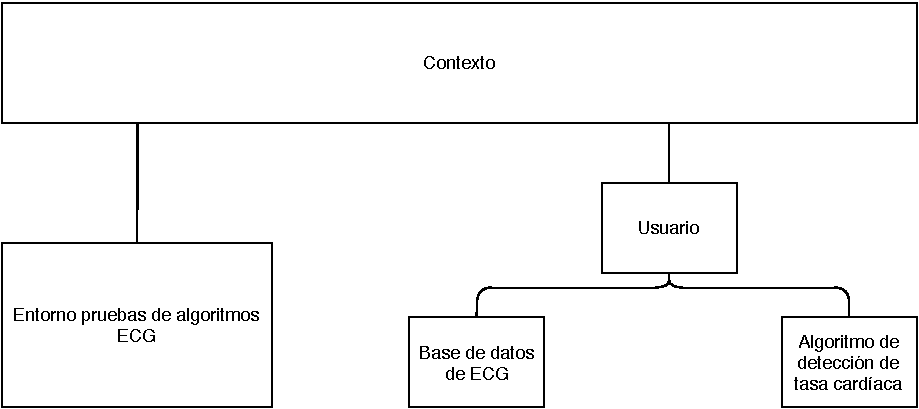
\includegraphics[width =\linewidth]{figuras/ContextDiagram.pdf}
        \caption{Diagrama de contexto}
        \label{fig:CtxDiagram}
    \end{figure}

    \subsection{Casos de uso}

    Una vez establecido el contexto en el que se desenvuelve el proyecto se pueden establecer los casos de uso. De nuevo se realiza un esquema para poder visualizarlos como conjunto. Este esquema puede verse en la figura \ref{fig:UseCasesDiagram}, en él se muestran las acciones que podría llevar a cabo el usuario una vez el proyecto esté finalizado, aunque será tarea futura determinar cuales gozan de mayor prioridad, pues no todas son iguales de fundamentales a la hora de llevar a cabo el objetivo principal del proyecto.

    \begin{figure}[H]  
        \centering
            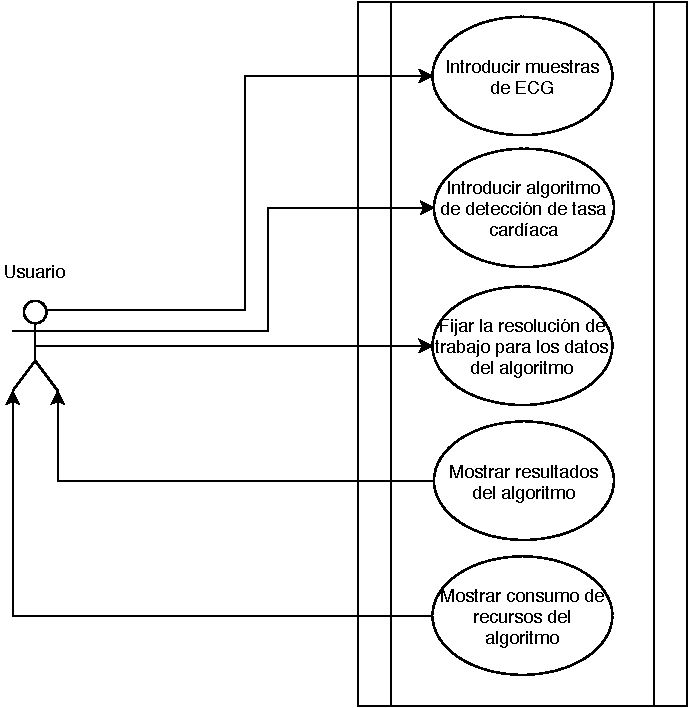
\includegraphics[width =0.7\linewidth]{figuras/UseCasesDiagram.pdf}
        \caption{Diagrama de casos de uso}
        \label{fig:UseCasesDiagram}
    \end{figure}

    Estando aclaradas estas interacciones ya resulta posible comenzar a establecer los requisitos del proyecto, sin embargo primero se debería establecer conceptualmente el flujo de trabajo que se llevará a cabo para el testeo de los algoritmos.

    \subsection{Flujo}

    De forma muy simplificada se puede observar en la figura \ref{fig:BlocksDiagram} el flujo de trabajo del entorno de pruebas. Este diagrama es útil para tener en mente en todo momento el objetivo del proyecto en su versión más simplificada.

    \begin{figure}[H]  
        \centering
            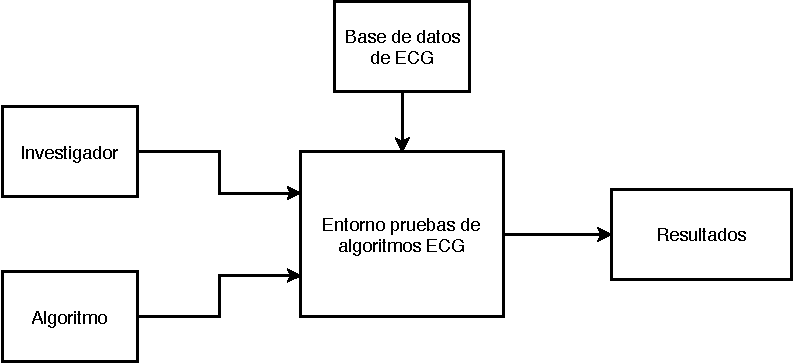
\includegraphics[width =\linewidth]{figuras/BlocksDiagram.pdf}
        \caption{Diagrama de bloques}
        \label{fig:BlocksDiagram}
    \end{figure}
    \clearpage


\section{Requisitos generales}

    Con la ayuda de los diagramas realizados se establecen los siguientes requisitos para cumplir con el objetivo establecido:
     
    \begin{scriptsize}
    \begin{longtable}{|p{0.05\linewidth}|p{0.21\linewidth}|p{0.3\linewidth}|p{0.3\linewidth}|p{0.03\linewidth}|}
        \hline
        ID & Requisito & Descripción & Prueba & Prio \\ \hline
        \endfirsthead
        %
        \endhead
        %
        \hline
        \endfoot
        %
        \endlastfoot
        %
        1 & Panel de control & El proyecto debe disponer de un panel de usuario intuitivo para llevar a cabo las pruebas &  & 1 \\ \hline
        1.1 & Introducir señal de prueba & Al panel de control se le debe proveer una señal de ECG formateada específicamente para poder probar el algoritmo deseado & Introducir un ECG extraído de alguna base de datos y comprobar que los valores de las muestras enviados se corresponden & 1 \\ \hline
        1.2     & Observar el comportamiento del algoritmo & Al panel de control se le debe proveer de gráficas de salida que muestren el estado de la señal procesada. & Observar las gráficas de salida y comprobar con un algoritmo predecible que el resultado obtenido es el deseado & 2 \\ \hline 
        1.3     & Resultados & El panel de control debe ser capaz de mostrar al usuario los siguientes elementos: &  &  \\ \hline
        1.3.1   & Frecuencia cardiaca instantánea & El panel deberá mostrar la frecuencia cardíaca instantánea medida por el algoritmo a testear. & Comprobar que el dato enviado por la aplicación de pruebas y el recibido por el panel son el mismo. La precisión de este no es un requisito pues dependerá del algoritmo con el que se esté trabajando. & 1 \\ \hline
        1.3.2   & Picos detectados & El panel deberá mostrar información sobre los picos R detectados y sus posiciones, para facilitar la evaluación del algoritmo & Al igual que la prueba anterior, se debe garantizar la coherencia de los datos entre la aplicación y el panel de usuario. La validez de estos dependerá del algoritmo. & 1 \\ \hline
        1.3.3   & Utilización del procesador instantánea & El panel deberá mostrar de forma instantánea el uso de CPU que corresponde al proceso del algoritmo de la forma más aproximada posible &  & 2 \\ \hline
        1.3.4   & Utilización de memoria instantánea & El panel deberá mostrar el uso de memoria en cada momento de la forma más aproximada posible &  & 2 \\ \hline
        1.3.5   & Fiabilidad del algoritmo & El panel deberá mostrar la fiabilidad (bien visual o bien en forma de tasas de falsos positivos y negativos) del algoritmo. & Contrastar con las anotaciones de la base de datos. & 2 \\ \hline
        1.4     & Resolución muestras & El panel deberá poder configurar la resolución empleada para las muestras en la aplicación, ofreciendo al usuario cierto control sobre la cantidad de muestras simultaneas con las que su algoritmo podrá trabajar. &  & 2 \\ \hline
        2       & Aplicación de pruebas & El proyecto debe disponer de una aplicación encargada de simular el comportamiento de un supervisor de eventos cardíacos introduciendo el algoritmo de detección de tasa cardíaca deseado. &  & 1 \\ \hline
        2.1     & Protocolo de comunicación & La aplicación debe ser capaz de recibir los datos desde el panel de usuarios y devolver los resultados procesados. & El correcto funcionamiento del resto de requisitos es prueba suficiente para este. & 1 \\ \hline
        2.2     & Entrada de datos en tiempo real & La aplicación debe enviar y recibir los datos en tiempo real para emular las condiciones de funcionamiento de un SEC. & Comprobar que la aplicación es capaz de recibir datos paulatinamente y devolverlos. & 1 \\ \hline
        2.2.1   & Simular la entrada de datos por el ADC & La aplicación debe simular la adquisición de datos mediante un conversor analógico digital. Emulando el funcionamiento de un supervisor real. & Comprobar que el acceso a esos datos está controlado con un Timer, como si del ADC se tratase. & 2 \\ \hline
        2.3     & Interfaz para el algoritmo & La aplicación debe disponer de una interfaz, dentro de la cual se pueda encapsular el algoritmo de detección de tasa cardíaca que el usuario desee probar. & Implementar dos algoritmos diferentes sin necesidad de modificar nada fuera de la interfaz. & 1 \\ \hline
        2.4     & Resolución muestras & La aplicación debe ser capaz de modificar la resolución empleada para las muestras en la aplicación, ofreciendo al usuario cierto control sobre la cantidad de muestras simultaneas con las que su algoritmo podrá trabajar. & Comprobar que el máximo de muestras almacenadas en el dispositivo varían en función de la calidad seleccionada en el panel de control. & 2 \\ \hline
        \caption{Requisitos iniciales}
        \label{tab:Requisitos}
    \end{longtable}        
    \end{scriptsize}
    
    Adicionalmente y para validar el sistema, se debe diseñar e implementar un algoritmo sencillo de detección de QRS. 
    \clearpage



\section{Metodología}

    Para la realización de este proyecto se ha decidido emplear una metodología de desarrollo ágil, en lugar de una metodología más tradicional como podría ser un desarrollo en cascada. El carácter iterativo e incremental de este tipo de diseño permite reaccionar más rápidamente a los cambios de diseño o nuevas necesidades que se encuentren durante el desarrollo.

    Uno de los marcos de trabajo ágiles más empleados en el desarrollo de software es el Scrum, que será empleado de una forma simplificada para el desarrollo de este proyecto. Dentro del Scrum nos encontramos tres figuras (Product owner, Scrum master y Equipo) sin embargo dado el carácter individual de este proyecto solo se emplearán dos. El product owner, representado por los tutores, que revisará el proyecto tras cada iteración y el desarrollador, encargado de organizar y llevar a cabo las iteraciones.

    \begin{figure}[H]  
        \centering
            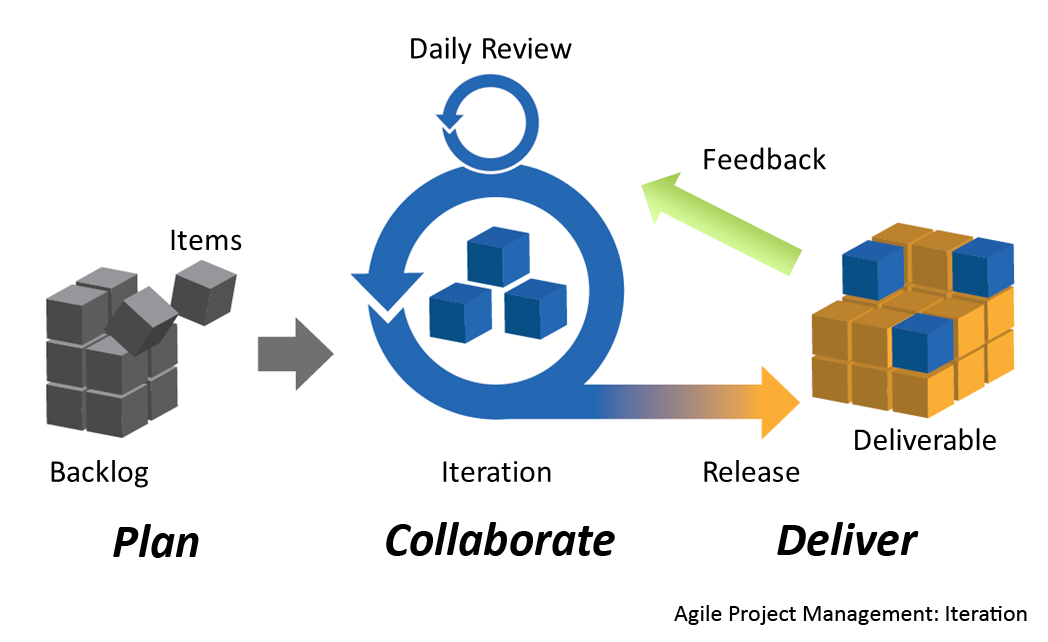
\includegraphics[width =0.9\linewidth]{figuras/Agile.png}
        \caption{Diagrama conceptual de la metodología ágil.}
        \label{fig:agile}
    \end{figure}

    Una iteración es la unidad fundamental de trabajo en una metodología ágil, y consiste en la adición de un nuevo fragmento de código que añade o mejora alguna función del proyecto, tratando de generar valor en cada iteración. Cada una de estas unidades de trabajo consta de su propia planificación, análisis de requisitos, diseño, codificación y su propia documentación.

    Dada la necesidad de agrupar toda la documentación generada del proyecto en un solo documento, en lugar de generar un fichero de documentación específico para cada iteración se clasificará cada iteración como un apartado del documento. El lector deberá tener en cuenta pues que los apartados referentes a las iteraciones del proyecto gozarán de una temporalidad y orden explícitos.
    
    Respecto a la metodología ágil, otro apartado imprescindible consiste en la realización de pruebas antes de finalizar cada iteración, asegurando el funcionamiento de cada pedazo de código añadido evitando la propagación de errores a lo largo del proyecto.
    
    Dada la naturaleza dual del proyecto se empleará una metodología de pruebas diferente para cada parte del proyecto. El panel de usuario será comprobado mediante ``Unit Testing'' o pruebas unitarias. Para el dispositivo de pruebas se empleará una directiva de compilación que incluirá o no el código de test en la compilación.

\clearpage

\chapterend{}


\chapterbegin{Implementación}
    \minitoc
    \clearpage
    %%%%%%%%%%%%%%%%%%%%%%%%%%%%%%%%%%%%%%%%%%%%%%%%%%%%%%%%%%%%%%%%%%%
%%% Documento LaTeX 																						%%%
%%%%%%%%%%%%%%%%%%%%%%%%%%%%%%%%%%%%%%%%%%%%%%%%%%%%%%%%%%%%%%%%%%%
% Título:		Capítulo 3
% Autor:  	Ignacio Moreno Doblas
% Fecha:  	2014-02-01, actualizado 2019-11-11
% Versión:	0.5.0
%%%%%%%%%%%%%%%%%%%%%%%%%%%%%%%%%%%%%%%%%%%%%%%%%%%%%%%%%%%%%%%%%%%
% !TEX root = A0.MiTFG.tex

\section{Iteración inicial: Planteamiento básico}
        \subsection{Resumen}
        
        Esta primera iteración consiste en la selección justificada del hardware y software en los que se basará todo el proyecto. Es importante tomar esta decisión pronto en el proceso de desarrollo porque limitará en gran medida las herramientas de las se dispondrá para todo el proyecto. Pero a su vez debe ser una elección sopesada ya que cambiar de tecnología en un futuro suele acarrear considerables problemas.
        
        \subsection{Desarrollo}

        El sistema consta de dos partes fundamentales. Primeramente un panel de control desde el cual un usuario podrá modificar los datos de entrada y observar los resultados del análisis de efectividad y eficiencia de los algoritmos. En segundo lugar debe existir un dispositivo físico, el cual lleve a cabo la ejecución de los algoritmos en tiempo real mientras realiza medidas de rendimiento sobre ellos.

        Para el panel de control se ha decidido emplear QT, concretamente la versión 4.9.0. Con esto se consigue evitar el tener que gestionar los componentes gráficos de la interfaz, pudiendo centrar el esfuerzo mayoritariamente en el tratamiento de los datos y las interacciones de usuario.
        
        Para el hardware del dispositivo en tiempo real se ha escogido una Tiva C Series (TM4C123GXL) por su relativa potencia y familiaridad con el dispositivo.        

        \subsection{Diagrama}

        Una vez especificados el hardware y software a emplear se vuelve posible, y necesario, profundizar en los diagramas realizados anteriormente añadiendo cuestiones ya específicas de la solución escogida para el desarrollo del proyecto. Teniendo en cuenta las características de la tecnología escogida se ha realizado el diagrama \ref{fig:InternalBlocksDiagram}, detallando el flujo de trabajo del sistema.

        \begin{figure}[H]  
            \centering
                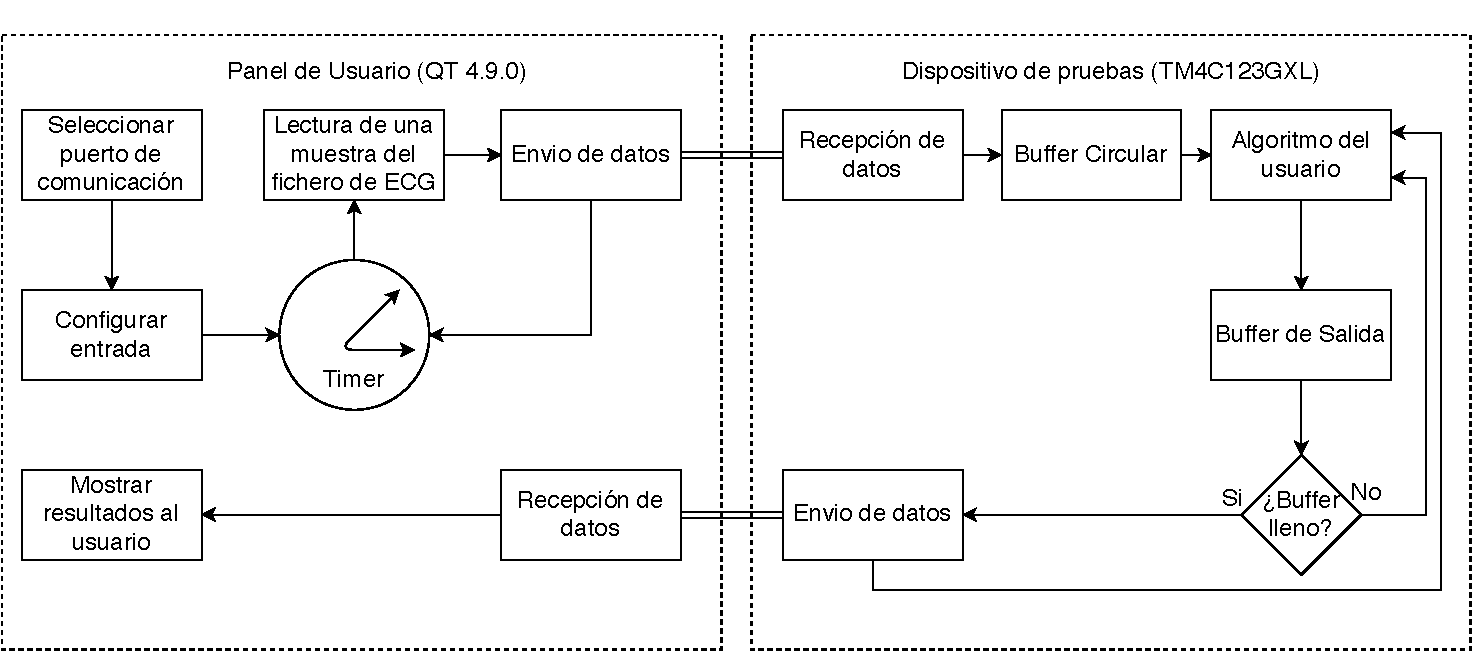
\includegraphics[width =\linewidth]{figuras/InternBlockDiagram.pdf}
                \caption{Diagrama de flujo de trabajo del sistema}
                \label{fig:InternalBlocksDiagram}
        \end{figure}
 
        La parte izquierda de la figura \ref{fig:InternalBlocksDiagram} representa la funcionalidad mínima necesaria para el panel de control y la parte derecha el flujo de trabajo del hardware de testeo. En un comienzo el factor ``Tiempo Real'' vendrá determinado por un \textit{timer} en el panel de control que enviará muestras del ECG de forma cíclica, a la frecuencia de muestreo que este se encuentre registrado, simulando así los tiempos biológicos reales de dichas señales. 
        
        Los datos son almacenados en un \textit{buffer} circular, el cual una vez lleno comenzará a sobrescribir los datos más antiguos. El algoritmo introducido deberá emplear únicamente los datos almacenados en el \textit{buffer} circular para llevar a cabo el análisis. Como en la vuelta de los datos no es tan importante simular el tiempo real se ha decidido devolverlos al panel en forma de paquetes, saturando menos el canal de comunicaciones.
        
        Una vez devuelta la información al panel de control, este deberá mostrar de alguna forma los datos al usuario que lo controla y además interpretar los resultados obtenidos para determinar la fidelidad del algoritmo y su eficiencia.        

        \subsection{Conclusiones}

        Las decisiones tomadas se han basado mayoritariamente en la familiaridad con las tecnologías escogidas, pero no por ello se ha desestimado lo apropiada que son para el alcance del proyecto.
        
        Decidida la estructura general del sistema, se puede comenzar la primera iteración de desarrollo, en la que se implementará la funcionalidad básica, sentando las bases para todo el desarrollo posterior.
    \clearpage
    %%%%%%%%%%%%%%%%%%%%%%%%%%%%%%%%%%%%%%%%%%%%%%%%%%%%%%%%%%%%%%%%%%%
%%% Documento LaTeX 																						%%%
%%%%%%%%%%%%%%%%%%%%%%%%%%%%%%%%%%%%%%%%%%%%%%%%%%%%%%%%%%%%%%%%%%%
% Título:		Capítulo 3
% Autor:  	Ignacio Moreno Doblas
% Fecha:  	2014-02-01, actualizado 2019-11-11
% Versión:	0.5.0
%%%%%%%%%%%%%%%%%%%%%%%%%%%%%%%%%%%%%%%%%%%%%%%%%%%%%%%%%%%%%%%%%%%
% !TEX root = A0.MiTFG.tex

\section{Primera iteración: El núcleo}
    \subsection{Resumen}

        Esta primera iteración está centrada en la codificación de la estructura básica de la aplicación, creando durante ella la infraestructura que servirá de apoyo para todas las funcionalidades que se implementen en las sucesivas iteraciones, llamado comúnmente como ``Core application''. 

        Para dar esta iteración por finalizada, la aplicación del panel deberá ser capaz de enviar las muestras de ECG hacia la plataforma de muestreo y está a su vez ser capaz de recibirlas y enviarlas de vuelta al panel, verificando así la comunicación en el doble sentido.

    \subsection{Requisitos}

        Los requisitos a realizar en esta iteración son el 1.1, el 2.2 y el 2.1 de la tabla de requisitos iniciales. (Tabla \ref{tab:Requisitos}) Estos requisitos dan lugar al siguiente desglose de tareas y subtareas:

        \begin{enumerate}
                \item Introducir señales de pruebas.
                \begin{enumerate}
                        \item Lectura de un fichero de datos con muestras de ECG.
                        \item Envío de las lecturas a la plataforma de testeo a la frecuencia original de muestreo.
                        \item Interfaz de usuario básica para gestionar la lectura del fichero.
                \end{enumerate}
                \item Entrada de datos en tiempo real.
                \begin{enumerate}
                        \item Buscar la manera de realizar el análisis de manera continuada sin dejar de recibir nuevos datos en el proceso.
                \end{enumerate}
                \item Protocolo de comunicación.
                \begin{enumerate}
                        \item Definir el protocolo de comunicación a emplear.
                \end{enumerate}
        \end{enumerate}

    \subsection{Desarrollo}

        Como ya se mencionó en el capítulo de Introducción, existen diversas bases de datos fisiológicos, concretamente en este proyecto se usa la MIT-BIH Arrythmia Database \cite{MIT-BIH}, que contiene  muestras de ECG anotadas por especialistas en cardiología y cuyo uso está ampliamente extendido. Es posible acceder a sus datos a través del repositorio de Physionet \cite{phisionet}, y, haciendo uso de su propia API, descargar los datos directamente desde matlab. De este modo, con un simple script, es posible convertir cualquier muestra de datos procedente de dicho repositorio en un fichero de texto estandarizado para la entrada de datos del entorno de pruebas.
        
         \code{Función de Matlab para extraer los datos del repositorio y formatearlos como texto.}{code/MatlabFirst.m}{code:sampleAsText}{Octave}

        El siguiente paso consiste en leer dichos ficheros de texto desde el panel de usuario y preparar los datos para enviarlos al dispositivo de pruebas. Este proceso tiene dos puntos claves, la lectura debe ser periódica y su frecuencia debe ser igual que la frecuencia de muestreo de las muestras. Para lograr este cometido se ha desarrollado un script siguiendo la estructura del diagrama \ref{fig:SimpleFileRead}. 

        \begin{figure}[H]  
                \centering
                        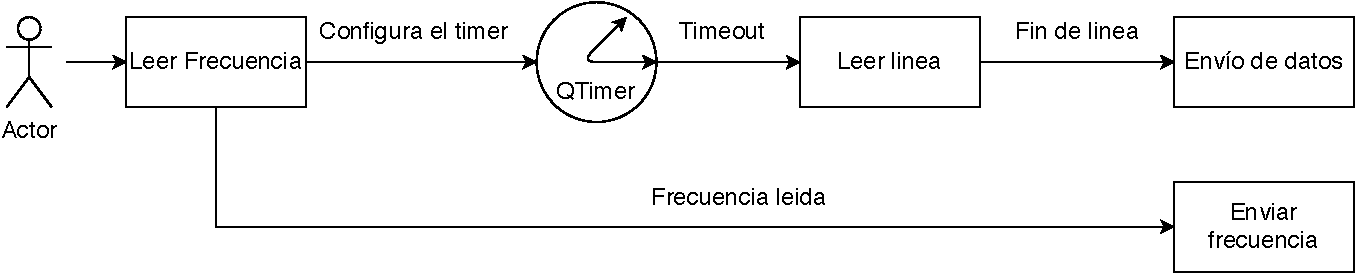
\includegraphics[width =\linewidth]{figuras/SimpleFileRead.pdf}
                \caption{Diagrama de lectura de ficheros simplificado}
                \label{fig:SimpleFileRead}
        \end{figure}

        Para sincronizar las partes del script y garantizar la compatibilidad con futuras funcionalidades del panel de control se hace uso de los SLOT y las SIGNAL de Qt. Estos elementos son el pilar fundamental de las aplicaciones desarrolladas con Qt ya que actúan como canales de mensajes, permitiendo la sincronización de todas las funciones de la aplicación sin caer en fuertes restricciones por acoplamiento de las diferentes funcionalidades. El concepto es sencillo, cuando sucede un evento se emite una SIGNAL concreta para dicho evento, que además puede incluir datos como parámetros, y cualquier número de SLOTS que estén configurados para recibir dicha SIGNAL se ejecutan en paralelo. 

        Como se puede ver en el diagrama \ref{fig:CompleteFileRead} se han añadido también diferentes entradas para que el usuario interaccione. Estas son una rueda selectora para configurar la frecuencia de forma manual, un botón para realizar la lectura de la frecuencia de muestreo directamente desde el fichero y un tercero que daría comienzo a la prueba. En la figura \ref{fig:frecKnob} se puede ver la disposición de estos elementos en el panel.

        \begin{figure} [H] 
                \centering
                        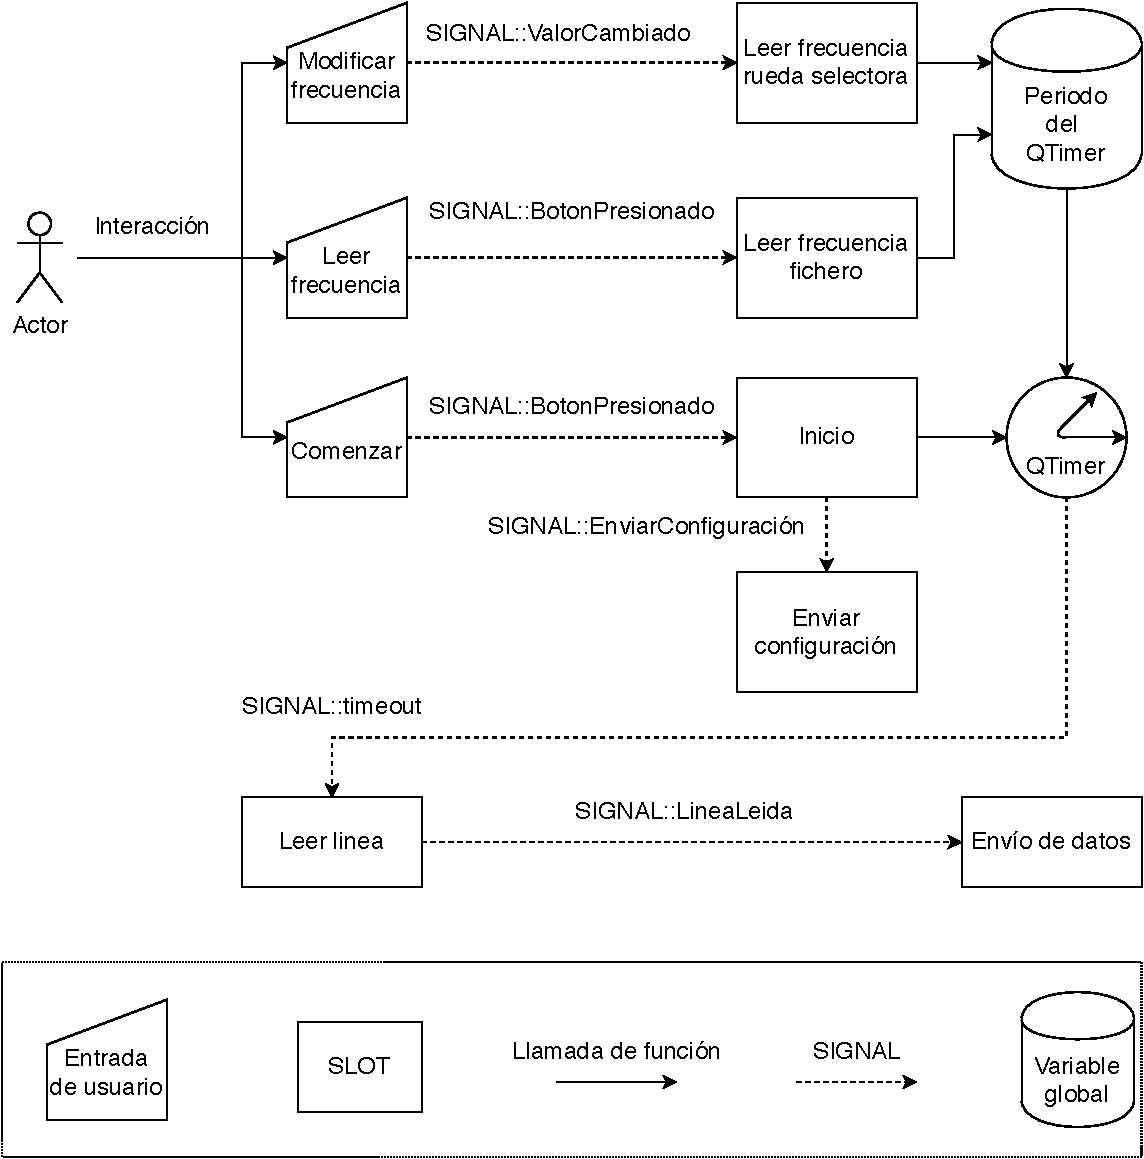
\includegraphics[width =\linewidth]{figuras/CompleteFileRead.pdf}
                \caption{Diagrama de lectura de ficheros en QT}
                \label{fig:CompleteFileRead}
        \end{figure}

        Antes de continuar con la implementación del envío de los datos, es necesario detenerse en la gestión del tiempo real y el sincronismo dentro del dispositivo de pruebas, concretamente la Tiva (TM4C123GXL). Para esta finalidad se ha hecho uso de un sistema operativo de tiempo real de software libre llamado FREERTOS (TODO: Cita). Gracias a él se pueden gestionar y sincronizar tareas asignándoles diferentes prioridades, solucionando el problema de tener que gestionar las comunicaciones a la vez que se realizan las pruebas de rendimiento, ganando en el proceso además total independencia entre las tareas reduciendo acoplamientos.
        
        \begin{figure}[H]
                \centering
                        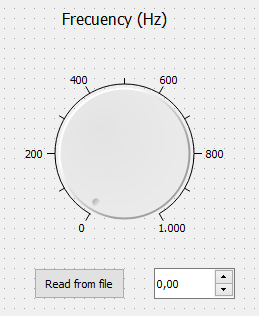
\includegraphics[width =0.4\linewidth]{figuras/FrecKnob.png}
                \caption{Selector de frecuencias y lectura del fichero}
                \label{fig:frecKnob}
        \end{figure}

        Para la comunicación entre el dispositivo de pruebas y el panel de usuario se hace uso de un puerto serie. Para garantizar la correcta transmisión de los datos se emplean dos mecanismos ampliamente extendidos por su eficacia y relativa sencillez, checksum y byte stuffing. 
        
        El checksum es el mecanismo encargado de comprobar que no hayan habido errores en la comunicación, para ello se calcula un número en función de los bytes de la trama y se adjunta a esta, de forma que al recibir los datos, puede repetirse la operación y comprobar ambos valores. 
        
        El byte stuffing por otro lado define un mecanismo por el cual se protegen los caracteres especiales de la trama. Por motivos azarosos es posible que alguno de los bytes enviados coincida con un byte reservado correspondiente a algún carácter especial  como podría ser el de fin de trama. El byte stuffing empleado en este proyecto consiste en la incorporación de un carácter especial de salto justo delante de cada carácter reservado que se localice. De esta forma, en recepción se puede tratar un carácter especial como un byte normal si frente a el se encuentra el carácter de salto. No existe ningún problema si la cadena original contiene un byte idéntico al carácter de salto, pues esto resultaría en la incorporación de un carácter de salto frente al original, tratando a este como un byte normal en recepción.
        
        Para complementar lo explicado sobre el protocolo de comunicación, este se ha representado en el diagrama \ref{fig:frame}. Cada salto de línea representa cada nueva etapa del protocolo de envío. El ejemplo expuesto contiene un byte de datos que coincide con el byte de final de trama, representado como “END”, a fin de ejemplificar el funcionamiento del método de stuffing.

        \begin{figure}[H]
                \centering
                        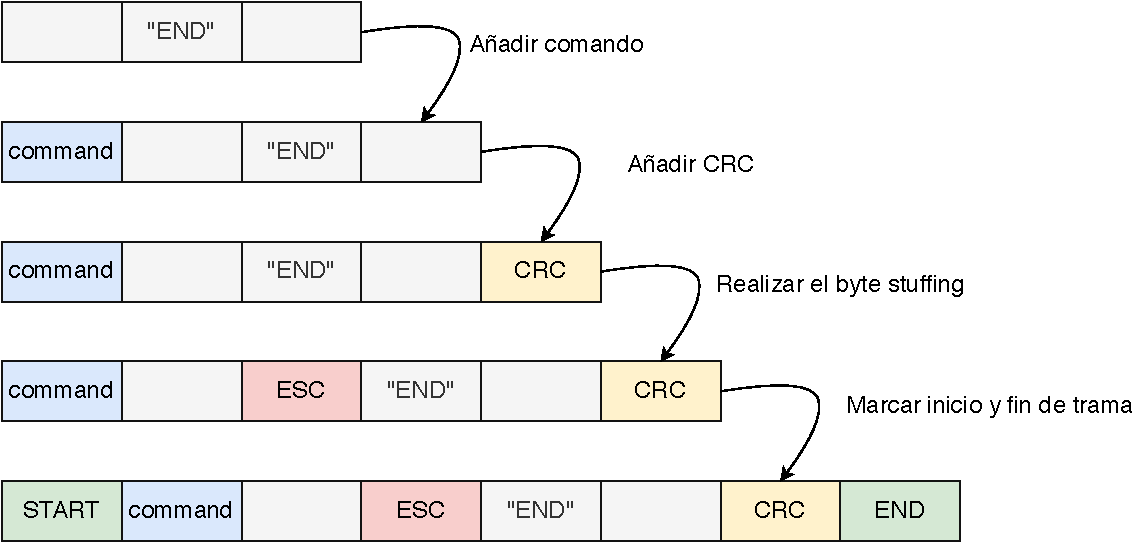
\includegraphics[width = \linewidth]{figuras/ProtocoloCom.pdf}
                \caption{Proceso construcción de trama}
                \label{fig:frame}
        \end{figure}

    \subsection{Pruebas}

        Para testear la lectura de ficheros en Qt se han implementado una serie de tests unitarios con el objetivo de verificar las lecturas correctas, pero además, de verificar que ante entradas de datos erróneas como ficheros mal formateados el sistema reacciona de forma correcta.

        Los casos sometidos a test han sido:

        \begin{itemize}
                \item Lectura correcta de la frecuencia desde el fichero
                \item Lectura incorrecta de la frecuencia desde el fichero
                \item Lectura correcta de una línea de datos
                \item Lectura incorrecta de una línea de datos
        \end{itemize}

        Para el protocolo el proceso ha sido similar, si es capaces de codificar y decodificar un mensaje, donde entre en juego la necesidad de emplear el bit Stuffing, entonces debe ser capaz de codificar y decodificar cualquier mensaje.

        Para comprobar la transmisión de los datos entre el panel y el dispositivo de prueba se ha optado por un test de carácter más empírico. Si se puede enviar en tiempo real y recibir de vuelta la señal deseada sin que los datos se distorsionen, se puede concluir que el sistema de transmisión funciona correctamente.

        (TODO: Imagen de los dos ECG)


    \subsection{Conclusiones}

        Tras la realización de esta iteración quedan sentadas las bases para el correcto desarrollo del proyecto. A su vez se hizo presente la necesidad de implementar una nueva funcionalidad.

        La inclusión de un mecanismo para que el usuario pueda seleccionar de manera fácil e intuitiva la muestra de señal que desea emplear para las pruebas. Esta funcionalidad ha sido incluida en la tabla de requisitos finales con el código 1.5. de la sección de conclusiones finales. (TODO: Referencia a la tabla final)

        De la realización de los test también se observó la necesidad de incluir algún tipo de mecanismo de mensajes para notificar a los usuarios los errores o advertencias que se produzcan en el panel de control. Esta funcionalidad se ha incluido en la tabla de requisitos finales con el código 1.6. de la sección de conclusiones finales (TODO: Referencia a la tabla)
        
    \clearpage
    %%%%%%%%%%%%%%%%%%%%%%%%%%%%%%%%%%%%%%%%%%%%%%%%%%%%%%%%%%%%%%%%%%%
%%% Documento LaTeX 																						%%%
%%%%%%%%%%%%%%%%%%%%%%%%%%%%%%%%%%%%%%%%%%%%%%%%%%%%%%%%%%%%%%%%%%%
% Título:		Capítulo 3
% Autor:  	Ignacio Moreno Doblas
% Fecha:  	2014-02-01, actualizado 2019-11-11
% Versión:	0.5.0
%%%%%%%%%%%%%%%%%%%%%%%%%%%%%%%%%%%%%%%%%%%%%%%%%%%%%%%%%%%%%%%%%%%
% !TEX root = A0.MiTFG.tex

\section{Segunda iteración: Funcionalidad básica}
    \subsection{Resumen}
        La segunda iteración gira en torno a la creación de un primer prototipo funcional que realice, aunque de forma parcial y poco intuitiva, las funciones deseadas para el producto final.

        Centrarse únicamente en la funcionalidad a esta altura del proyecto favorece a reducir el tiempo invertido en pulir detalles que no son realmente necesarios en esta fase tan temprana, economizando el tiempo de desarrollo.

    \subsection{Requisitos}
        Los requisitos a realizar en esta iteración son el 1.3.1, el 1.3.2 y el 2.3 de la tabla de requisitos iniciales (Tabla \ref{tab:Requisitos}). Además, derivado de la iteración anterior, se va a implementar el requisito 1.5 de la tabla completa. (TODO: Cita tabla final). Estos requisitos dan lugar a las siguientes tareas:
    
        \begin{enumerate}
            \item Implementar un mecanismo por el que seleccionar el fichero de entrada.
            \item Implementar la interfaz para los algoritmos de detección.
            \begin{enumerate}
                \item Almacenar la señal de entrada en un buffer.
                \item Definir la interfaz
            \end{enumerate}
            \item Mostrar los resultados del análisis en el panel de usuario.
        \end{enumerate}
        
    \subsection{Desarrollo}
        
        La primera tarea se ha resuelto mediante el empleo de un "QListView"  (TODO:  referencia https://doc.qt.io/archives/qt-4.8/qlistview.html) al que se le ha configurado una carpeta raíz donde se colocarán todos los ficheros de datos junto con unos filtros para que solo muestre estos. Haciendo uso del SLOT \char`_clicked se puede obtener la ruta al fichero que clickea el usuario dentro del widget, permitiendo pasarla como parámetro a la función de lectura implementada en la anterior iteración. 
        
        \begin{figure}[H] 
                \centering
                        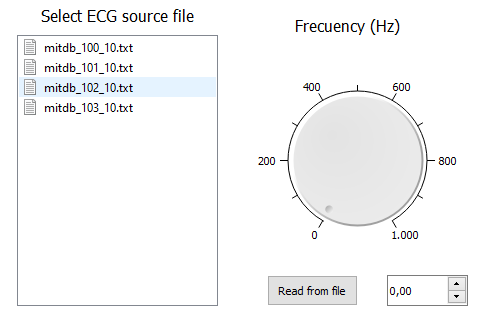
\includegraphics[width = 0.8 \linewidth]{figuras/fileView.png}
                \caption{Estado de la configuración en el panel de control tras la finalización de la segunda iteración.}
                \label{fig:fileView}
        \end{figure}
        
        Para la tarea 2.a se ha implementado un buffer circular empleando una estructura que contiene un array de tipo int32 de 1024 posiciones y una variable para indicar el índice 0 relativo llamada “Head”, una vez inicializado este índice apunta al espacio de memoria donde está almacenado el dato más reciente. Además se proveen dos funciones auxiliares encargadas de introducir y leer elementos del buffer respecto a la posición de la variable Head. 
        
        La función encargada de introducir nuevas muestras modifica el Head del buffer para mantener el estado actualizado, su funcionamiento se explica en el diagrama \ref{fig:bufferDiagramAppend}. 
    
        \begin{figure}[H] 
                \centering
                        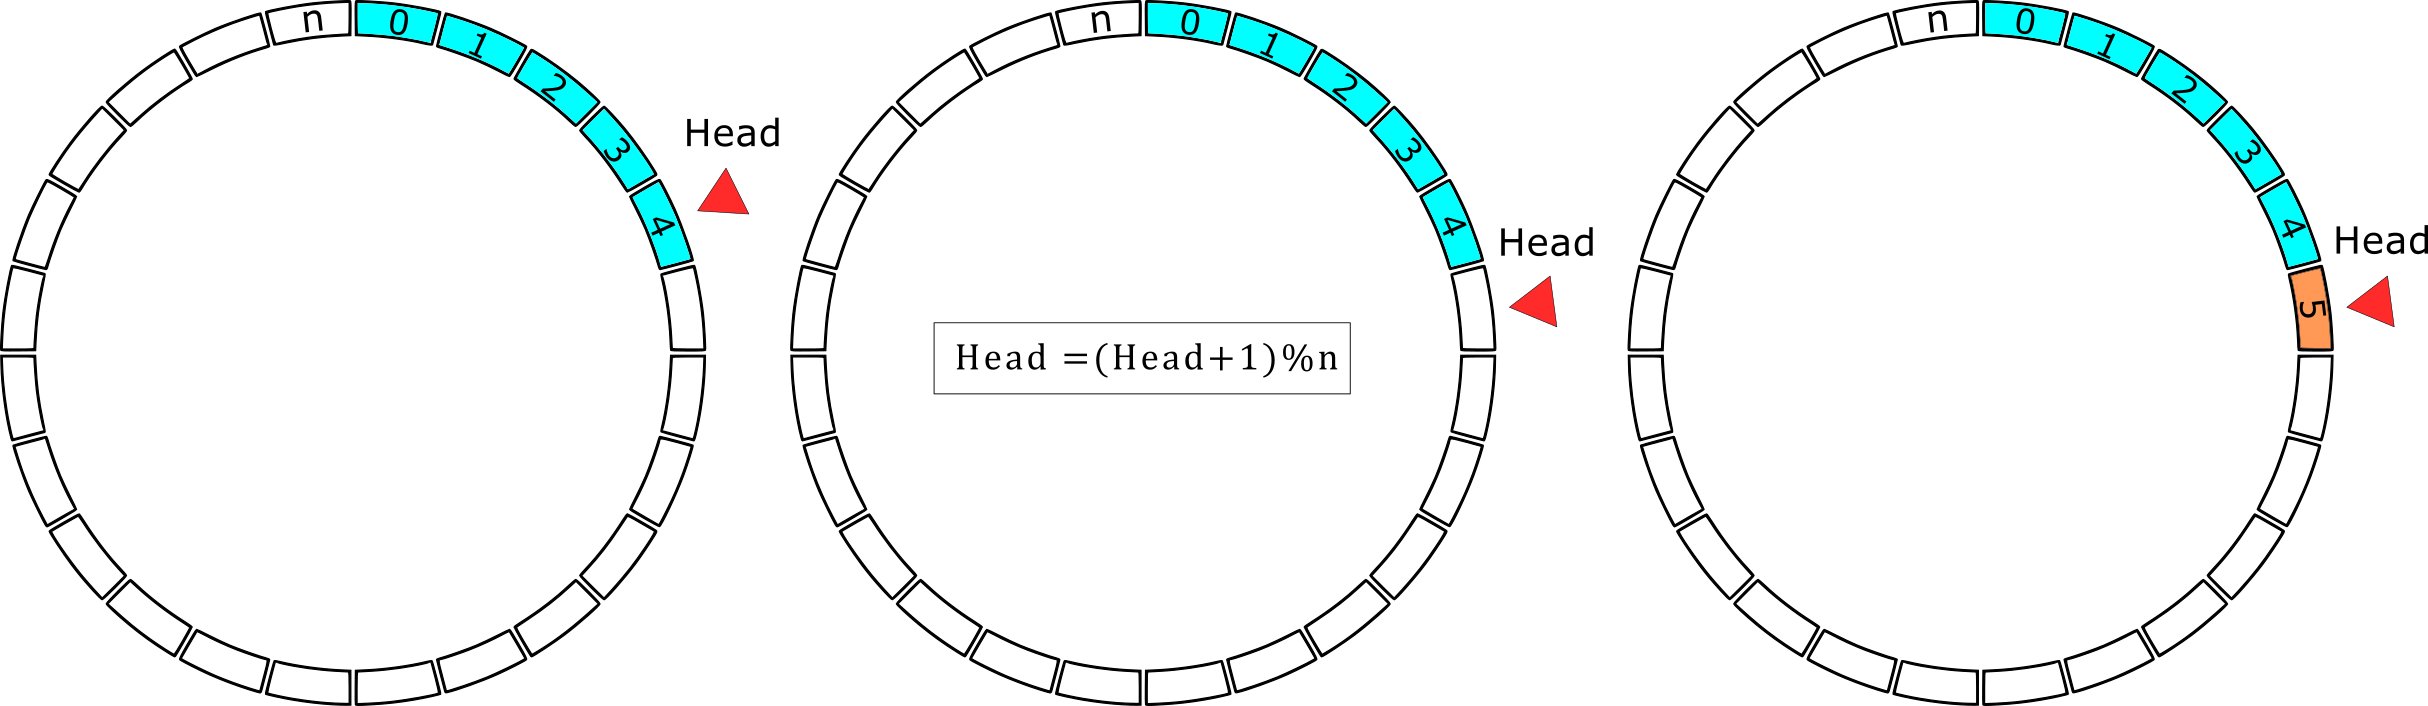
\includegraphics[width = \linewidth]{figuras/bufferAppend.png}
                \caption{Funcionamiento de \char`"AppendSample", función encargada de introducir muestras en el buffer.}
                \label{fig:bufferDiagramAppend}
        \end{figure}
        
        La función encargada de extraer las muestras simplemente recorre el array de forma relativa a la posición del Head como si se tratara de un array normal, retirando del usuario la necesidad de controlar los límites de este. Su funcionamiento está explicado en el diagrama \ref{fig:bufferDiagramGet}.
        
        \begin{figure}[H]
                \centering
                        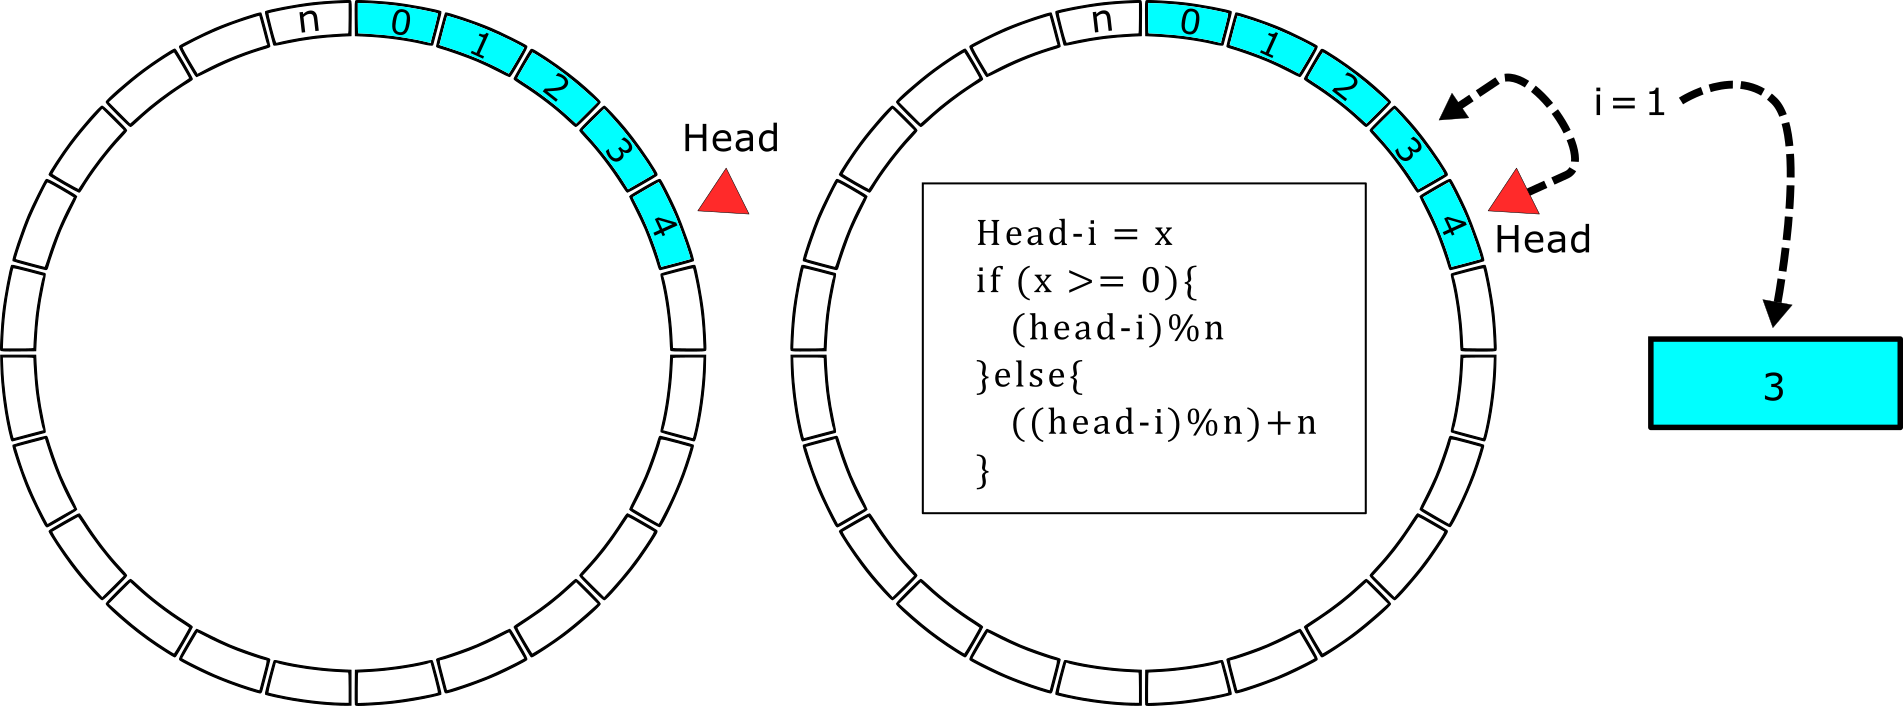
\includegraphics[width = 0.9 \linewidth]{figuras/bufferGet.png}
                \caption{Funcionamiento de "GetSample", función en cargada de extraer las muestras del buffer.}
                \label{fig:bufferDiagramGet}
        \end{figure}
        
        Respecto a la tarea 2.b, si bien no es posible generar una Interfaz propiamente dicha por ser un concepto de programación orientada a objetos, lo que se trata de lograr es limitar todas las modificaciones que deberá hacer un futuro usuario para introducir su algoritmo a un solo fichero, evitando la necesidad de modificar las llamadas a las funciones en otros ficheros de código. 

        La implementación se ha realizado mediante punteros a funciones. Se ha definido un tipo correspondiente a un puntero a una función con la firma establecida. De esta forma el usuario puede asignar al puntero cualquier función que desarrolle mientras satisfaga la firma impuesta por el mismo, haciendo las veces de interfaz.
        
        En la figura \ref{fig:functionPointer} puede observarse de forma compacta la implementación del funcionamiento previamente descrito. 

        \begin{figure}[H]
                \centering
                        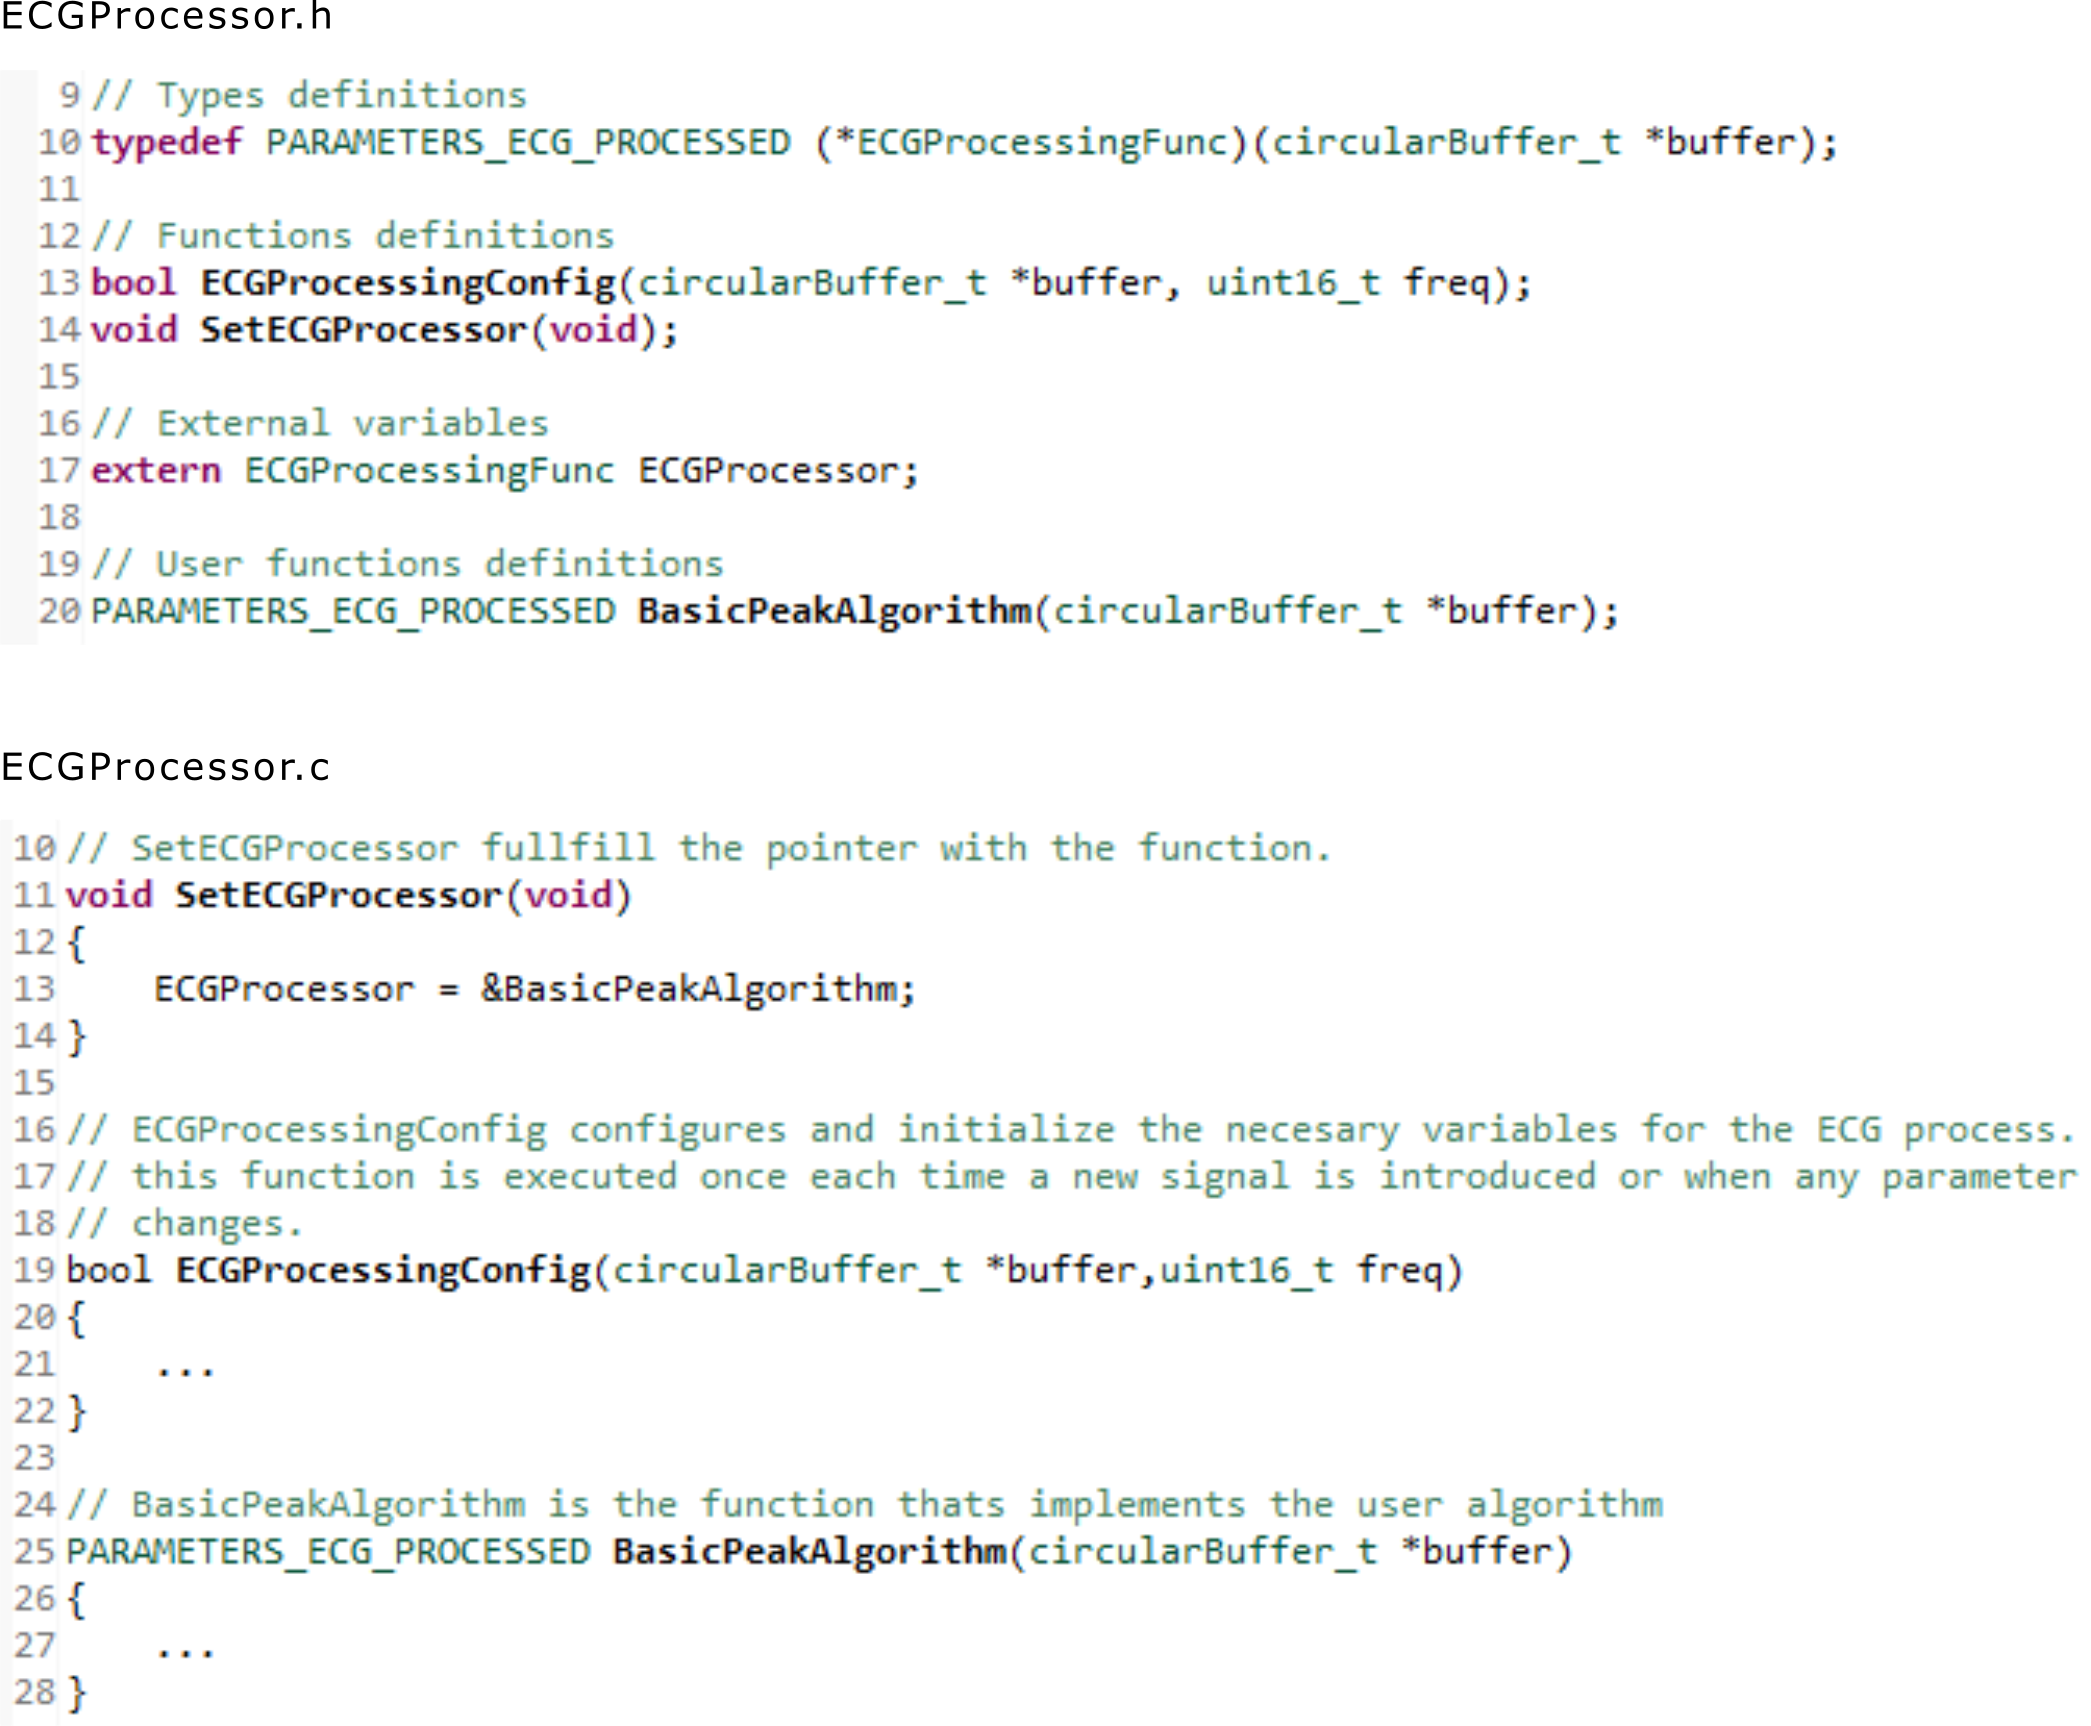
\includegraphics[width =\linewidth]{figuras/FunctionPointer.PNG}
                \caption{Gráfica que muestra los resultados del análisis llevado a cabo por el algoritmo.}
                \label{fig:functionPointer}
        \end{figure}
        

        Para la tercera tarea se han decidido implementar varios mecanismos para mostrar los resultados al usuario. Se ha añadido una gráfica empleando el widget QwtPlot donde se muestra la señal ECG leída del fichero en tiempo real. Sobre ella se dibujan los picos R detectados por el algoritmo. Además se ofrece la posibilidad de dibujar el threshold de detección si el algoritmo emplea uno y un recuadro donde se muestra el valor de la tasa cardíaca instantánea medida. En la figura \ref{fig:resultsBasic} puede observarse el formato de salida.

        \begin{figure}[H]
                \centering
                        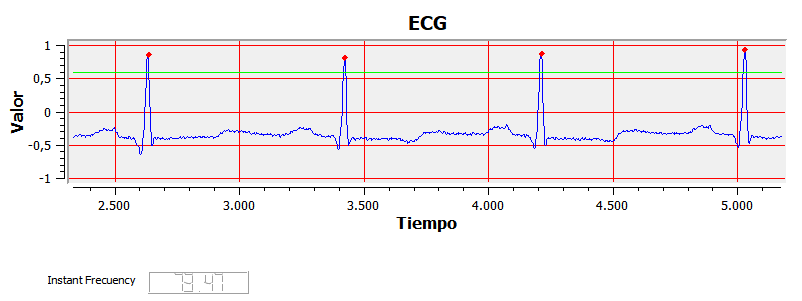
\includegraphics[width =\linewidth]{figuras/ResultsBasic.png}
                \caption{Gráfica que muestra los resultados del análisis llevado a cabo por el algoritmo.}
                \label{fig:resultsBasic}
        \end{figure}
        
    \subsection{Pruebas}
        
        La prueba de la tarea 1 de esta iteración se ha realizado simplemente proveyendo al programa con dos ficheros diferente y mediante el selector leer sus frecuencias. Puesto que la lectura de la frecuencia desde un fichero estaba testeada desde la iteración anterior, esto es suficiente para probar el funcionamiento del selector de ficheros.La figura \ref{fig:fileSelectorTest} se adjunta como prueba del test.

        \begin{figure}[H]
                \centering
                        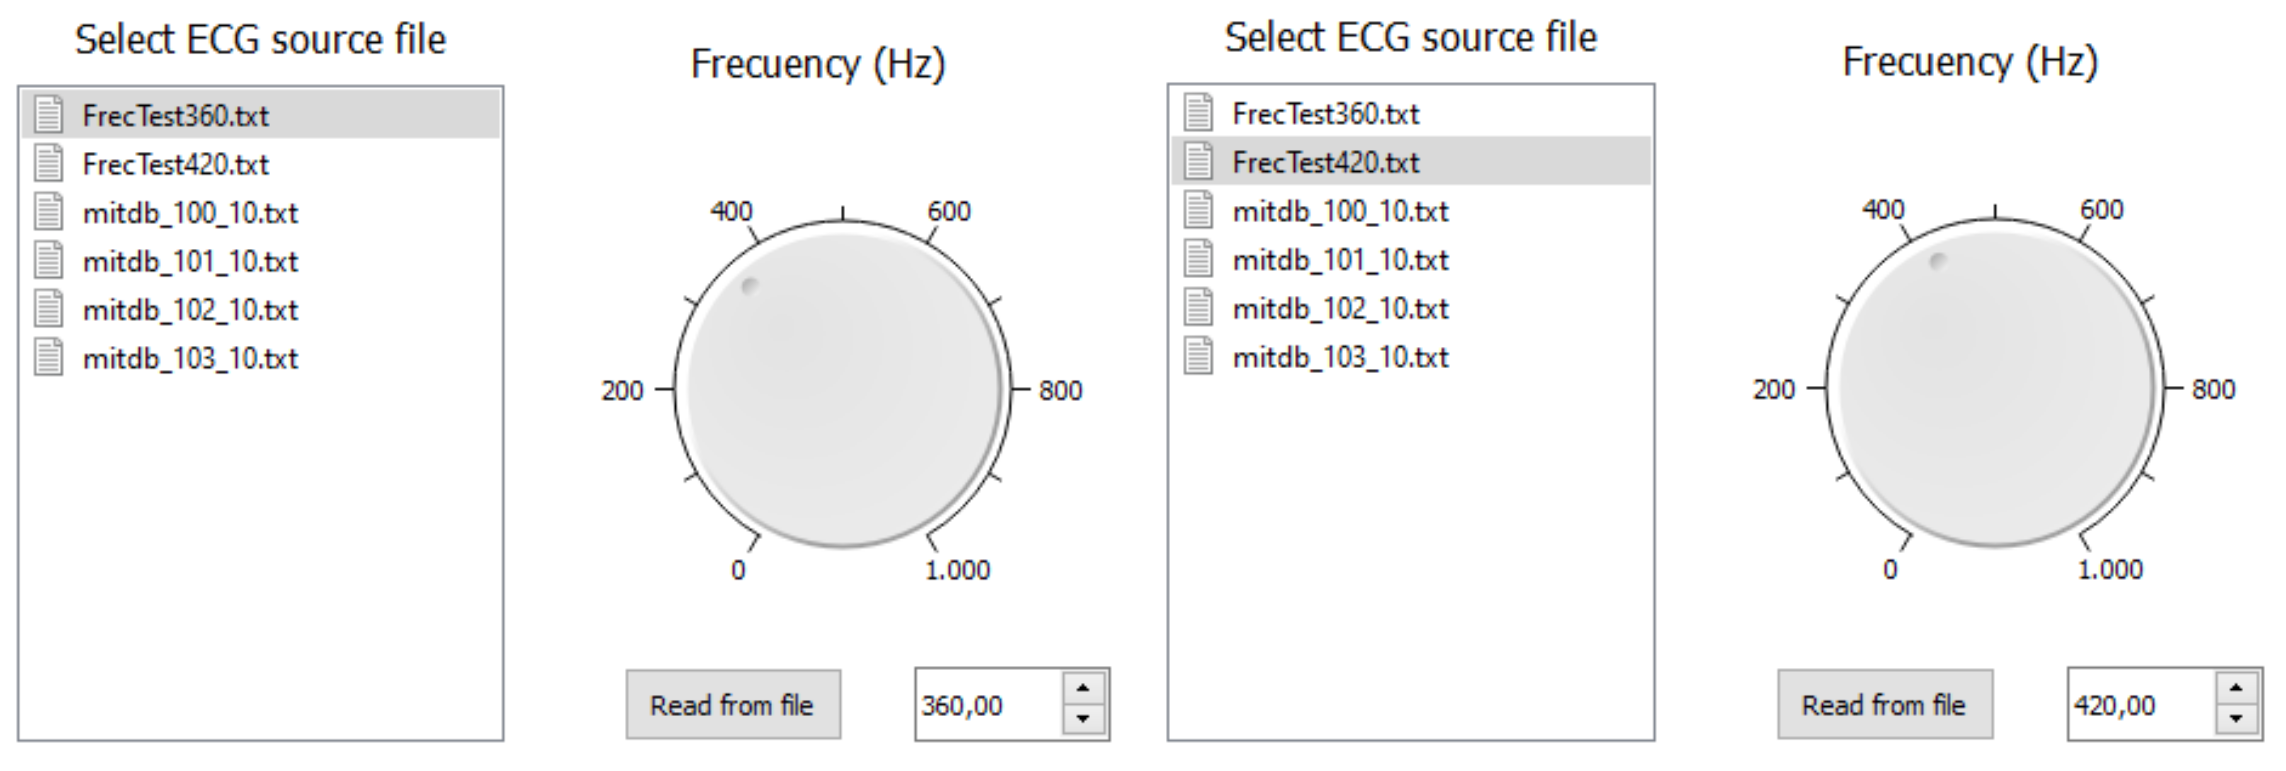
\includegraphics[width = \linewidth]{figuras/FileSelectorTest.png}
                \caption{Lectura de diferentes ficheros desde el selector.}
                \label{fig:fileSelectorTest}
        \end{figure}

        TODO: Escribir un test del buffer

        Para testear la interfaz, o mejor dicho, el puntero a una función simplemente se ha ejecutado el código en modo debug y comprobado que en el momento apropiado este ejecutaba la función correctamente mediante un punto de ruptura. 

        El test correspondiente al envío de los resultados de vuelta al panel resulta ser más sencillo de lo que pueda parecer a priori. Pues el envío correcto de los datos no implica que los datos sean correctos, por lo que no es necesario tener de momento un algoritmo capaz de detectar eficazmente la tasa cardiaca. Comprobando mediante puntos de ruptura que el dato enviado y recibido son el mismo y chequeando visualmente que el dato mostrado también es coherente puede darse por concluida esta prueba.

        
    \subsection{Conclusiones}
    
        Con la finalización de esta iteración queda definida la funcionalidad general, sin embargo para gozar de un primer prototipo cerrado es necesario llevar a cabo algunos cambios en el futuro cercano.
        
        Actualmente la interfaz para el algoritmo se ejecuta dentro de la rutina de recepción de los mensajes. Aunque es capaz de llevar a cabo todas la funciones que se le requieren sería más óptimo separar el procesado de la señal en una tarea aparte gestionada por el sistema operativo. Con esto se conseguiría además aislarla para simplificar la medida del rendimiento, permitiendo además emplear los propios mecanismos de FreeRTOS (TODO: Referencia a estos mecanismos) para realizar las medidas de rendimiento necesarias.
        
        Esta modificación se incluye como requisito en la tabla final (TODO: Referencia a la tabla final de requisitos) con el código: 2.5, aislamiento del procesado de señal.
    \clearpage
    %%%%%%%%%%%%%%%%%%%%%%%%%%%%%%%%%%%%%%%%%%%%%%%%%%%%%%%%%%%%%%%%%%%
%%% Documento LaTeX 																						%%%
%%%%%%%%%%%%%%%%%%%%%%%%%%%%%%%%%%%%%%%%%%%%%%%%%%%%%%%%%%%%%%%%%%%
% Título:		Capítulo 3
% Autor:  	Ignacio Moreno Doblas
% Fecha:  	2014-02-01, actualizado 2019-11-11
% Versión:	0.5.0
%%%%%%%%%%%%%%%%%%%%%%%%%%%%%%%%%%%%%%%%%%%%%%%%%%%%%%%%%%%%%%%%%%%
% !TEX root = A0.MiTFG.tex

\section{Tercera iteración: Rendimiento}
    \subsection{Resumen}
        
        Con esta iteración se pretende añadir todo lo referente a las mediciones de rendimiento del algoritmo. Tratando de concluir el prototipo inicial. Esta iteración aún se centrará exclusivamente en la funcionalidad del proyecto dejando de lado todas las cuestiones referentes a diseño de interfaces y experiencia de usuario para iteraciones posteriores.
        
    \subsection{Requisitos}

        Los requisitos a realizar en esta iteración son el 1.3.3 y el 1.3.4 de la tabla inicial (Tabla \ref{tab:Requisitos}) junto al requisito 2.5 de la tabla completa \ref{tab:RequisitosFinales} añadido durante la iteración anterior. Para ello se divide el trabajo de la iteración en las siguientes tareas:

        \begin{enumerate}
            \item Aislamiento del procesado de señales en una tarea exclusiva.
            \item Extraer las medidas de rendimiento del sistema operativo.
            \item Mostrar dichas medidas en el panel de usuario de QT.
        \end{enumerate}
        
    \subsection{Desarrollo}
        
        Para realizar la primera tarea de esta interación, \textit{aislamiento del procesado de señales}, el procesado de la señal se ha movido de la rutina encargada de manejar las comunicaciones, donde se alojaba inicialmente de forma provisional, a una tarea propia, desde la que resulta más sencillo calcular el tiempo de procesado y determinar los recursos que están siendo consumidos por la misma. Además, independizar estas dos tareas también ayuda a descongestionar las comunicaciones entre el dispositivo y el panel de control. Sin embargo, con la adición de las funciones necesarias para el funcionamiento de la tarea, se carga de contenido el fichero que finalmente será editable por el usuario, por este motivo, se ha decidido crear un fichero dedicado exclusivamente a las funciones del usuario llamado UserEntry.c y su correspondiente fichero de encabezado UserEntry.h, facilitando así la implementación de los algoritmos a evaluar. 
        
        Con los cambios incurridos en esta tarea, el diagrama de flujo del ciclo de trabajo del dispositivo de pruebas queda conforme a la figura \ref{fig:tivaFlow}. Aunque se debe tener en cuenta que en realidad las diferentes tareas mostradas en el diagrama no se ejecutan de forma perfectamente secuencial. El diagrama es solo una representación gráfica del flujo de una iteración completa de la ejecución en un caso ideal. En la realidad es posible que lleguen comandos mientras se ejecuta el algoritmo de detección. Para gestionar estas interrupciones el sistema operativo usa las prioridades.
        
        \begin{figure}
                \centering
                        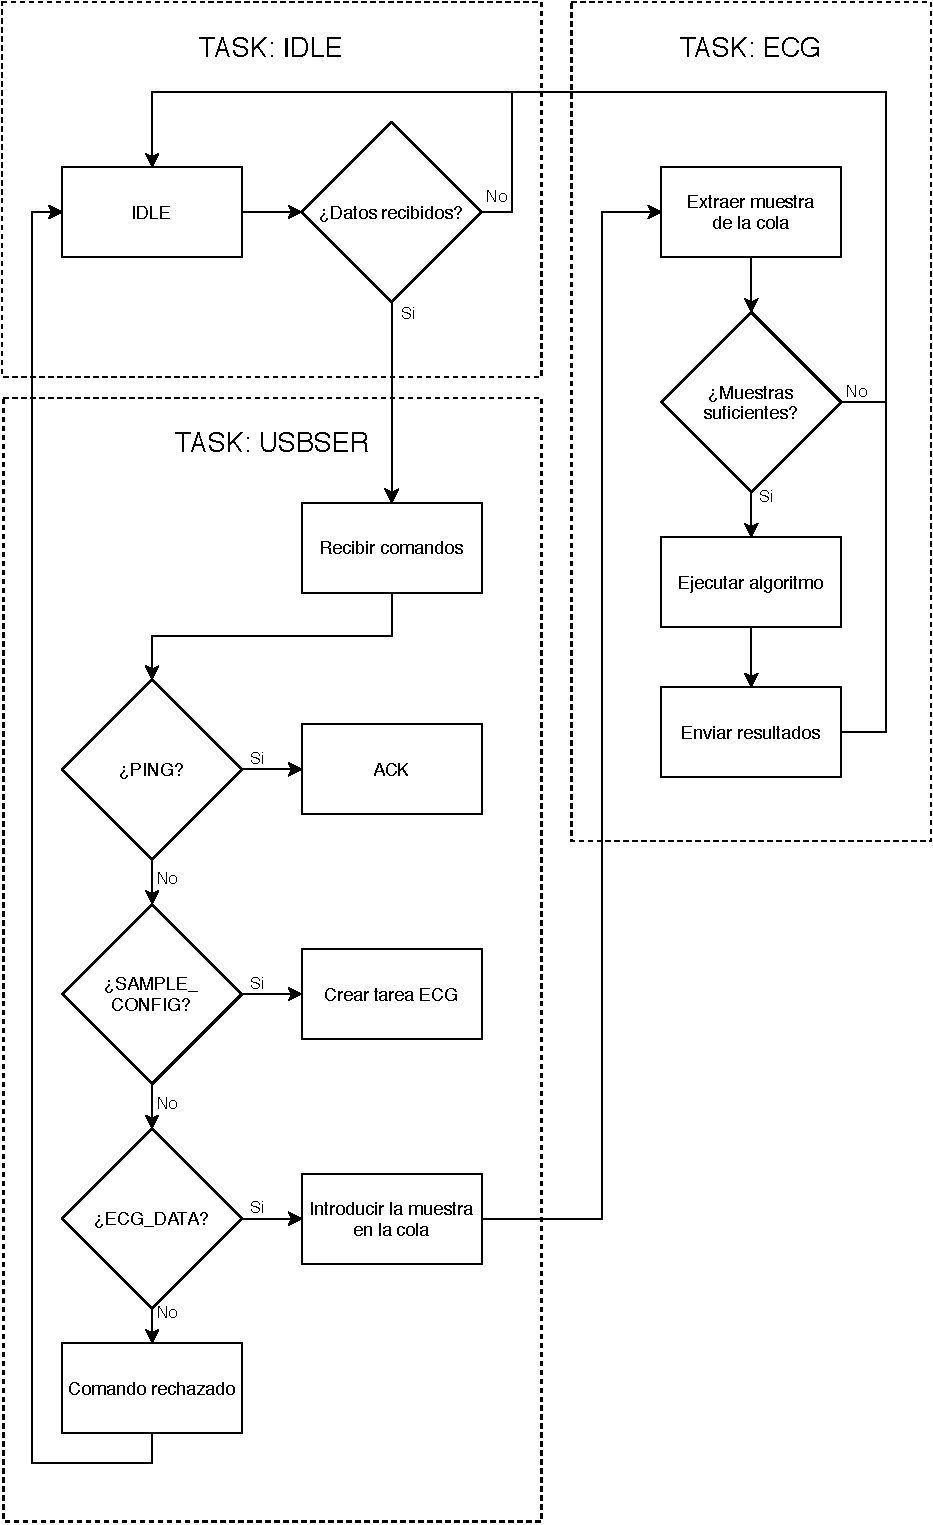
\includegraphics[width = 0.78 \linewidth]{figuras/TivaWorkFlow.pdf}
                \caption{Diagrama de flujo orientativo de las tareas en ejecución del dispositivo de pruebas.}
                \label{fig:tivaFlow}
        \end{figure}
        
        Para la segunda tarea, \textit{extracción de las medidas de rendimiento}, se han empleado dos mecanismos. 
        Por un lado, un Timer de alta frecuencia del dispositivo para contar el número de ciclos de reloj empleados en llevar a cabo cada ciclo de ejecución del algoritmo. El Timer empleado es el Timer4 configurado en modo cuenta periódica de 32 bits ascendente. Para realizar la medida al comienzo de cada ciclo de procesado se le asigna el valor 0 y cuando el procesado concluye se consulta la cuenta del temporizador, siendo esta equivalente al numero de ciclos de reloj transcurridos en el proceso. Si este valor se divide entre la frecuencia del mismo se obtiene una medida del tiempo empleado. Estos datos son los que aparecerán en la interfaz de usuario como ``Processing Tick'' y ``Processing Time (ms)''. La implementación puede observarse en el extracto \ref{code:timer}.
        
        \code{Implementación del Timer de diagnóstico.}{code/timer.cpp}{code:timer}{C++}
        
        Por otro lado,  también se hace uso de la función ``vTaskGetInfo()'' \cite{FreeRTOS}, perteneciente al sistema operativo, para extraer datos del estado de la CPU y el uso de memoria de la tarea de procesado. Estos datos aparecen en la interfaz de usuario como ``CPU usage (\%)'' y ``Memory left'', respectivamente .A diferencia del tiempo medido con el timer, los datos de uso de CPU extraídos con esta función no son exactos, pero, en principio, si suficientes para dar una idea general de la carga de trabajo. Respecto a la memoria, se indica la cantidad de memoria libre de la que dispone la tarea, por lo que valores altos son ideales, si este número llegara a cero significaría que la tarea se ha desbordado. 
        
        Para la tercera tarea, \textit{mostrar las medidas de rendimiento al usuario en el panel}, primero era necesario enviarlas, y para ello se ha decidido emplear otro paquete diferente al de los resultados del algoritmo. De esta forma se evita sobrecargar un paquete que ya es de por sí bastante grande y además se consigue independencia, previendo que en alguna iteración posterior se puedan añadir nuevos indicadores de rendimiento, que pueden incluso no depender de la ejecución del algoritmo.
        
        Respecto a la visualización de los datos de rendimiento, de momento solo se han añadido las salidas de texto correspondiente con la mínima explicación necesaria, posponiendo los detalles de interfaz de usuario para más adelante. Los valores son expuestos de manera visual y agrupada para su fácil comprensión, siguiendo el ejemplo de la figura \ref{fig:performance}.
        
        \begin{figure}[H]
                \centering
                        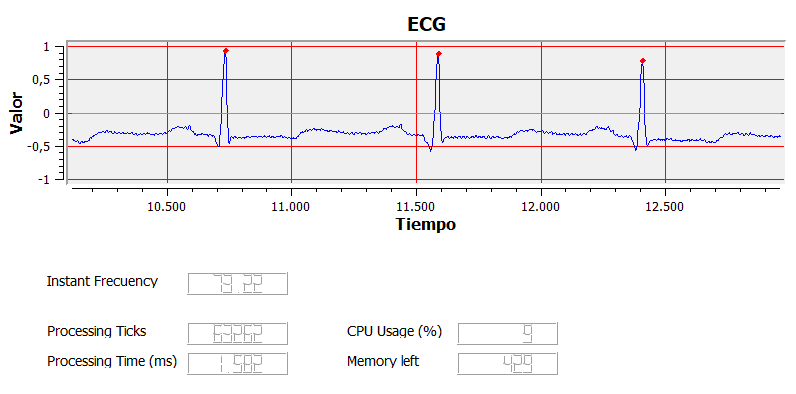
\includegraphics[width = 0.9 \linewidth]{figuras/Performance.PNG}
                \caption{Visualización de los datos de rendimiento.}
                \label{fig:performance}
        \end{figure}
        
    \subsection{Pruebas}
        
        De las tareas realizadas en esta iteración, la única que requiere de pruebas es la extracción de los datos de rendimiento de la CPU,usando la implementación del timer. Para ello se ha empleado la función ``SysCtlDelay()'' capaz de introducir un retardo fijo en la ejecución de una tarea. Midiendo el tiempo introducido por dicha función empleando el timer podemos obtener garantías de que la medida se está llevando a cabo correctamente. Como se puede ver en la figura \ref{fig:performanceTest} la medición obtenida es coherente con los datos introducidos.
        
        Se debe mencionar en este punto, que, después de invertir bastante tiempo en las funciones de diagnostico del sistema operativo en tiempo real para realizar las medidas de rendimiento, estas han demostrado ser bastante imprecisas. Especialmente aquellas dedicadas a medir las cargas de CPU (CPU Usage \%). La razón es que todas se basan en las medidas de un contador desde el momento en que se inició el sistema, por lo que si las tareas no se ejecutan a pleno rendimiento desde el comienzo, los promedios van a estar muy desviados de la realidad, o por el contrario, van a tardar bastante tiempo en dar un resultado estable.
        
        \begin{figure}[H]
                \centering
                        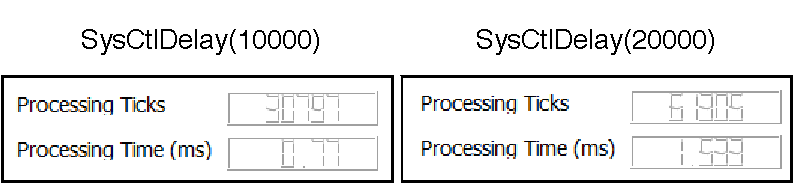
\includegraphics[width = 0.9 \linewidth]{figuras/PerformanceTest.pdf}
                \caption{Prueba medición tiempo de ejecución del algoritmo.}
                \label{fig:performanceTest}
        \end{figure}

    \subsection{Conclusiones}
    
    Con la finalización de esta iteración queda implementada la capacidad de valorar los algoritmos de detección empleados en función de los recursos empleados y su tiempo de ejecución, repercutiendo esta última directamente en el consumo de batería.
    
    En esta ocasión no han surgido nuevos requisitos que añadir, señal de que el proyecto está bien encauzado y de que la base establecida en las iteraciones anteriores es adecuada para el sistema.
    \clearpage
    %%%%%%%%%%%%%%%%%%%%%%%%%%%%%%%%%%%%%%%%%%%%%%%%%%%%%%%%%%%%%%%%%%%
%%% Documento LaTeX 																						%%%
%%%%%%%%%%%%%%%%%%%%%%%%%%%%%%%%%%%%%%%%%%%%%%%%%%%%%%%%%%%%%%%%%%%
% Título:		Capítulo 3
% Autor:  	Ignacio Moreno Doblas
% Fecha:  	2014-02-01, actualizado 2019-11-11
% Versión:	0.5.0
%%%%%%%%%%%%%%%%%%%%%%%%%%%%%%%%%%%%%%%%%%%%%%%%%%%%%%%%%%%%%%%%%%%
% !TEX root = A0.MiTFG.tex

\section{Cuarta iteración: Fiabilidad}
    \subsection{Resumen}
        
        En esta iteración se ha implementado todo lo relacionado con el cálculo de la fiabilidad del algoritmo siguiendo las indicaciones de la norma UNE-EN 60601-2-47:2002. Una vez concluida esta fase del desarrollo el proyecto ya será plenamente funcional. Aunque se deja para una etapa posterior lo relacionado con la interfaz de usuario.
        
    \subsection{Requisitos}
    
        Para esta iteración solo se pretende satisfacer un requisito, el 1.3.5 de la tabla inicial (tabla \ref{tab:Requisitos}). Para ello se ha dividido el requisito en las diferentes tareas:
        
        \begin{enumerate}
            \item Extraer las anotaciones de la base de datos y añadirlas al fichero de entrada.
            \item Implementar el control de las anotaciones en el panel de usuario.
            \item Crear un modelo de almacenamiento para las anotaciones que facilite la implementación de la norma (TODO: Norma de las evaluaciones)
            \item Implementar las ecuaciones descritas en la norma (TODO: Norma de las evaluaciones)
            \item Mostrar al usuario los resultados de la validación del algoritmo.
        \end{enumerate}
    
    \subsection{Desarrollo}
        Aunque pueda parecer simple, medir la eficiencia de un algoritmo de detección QRS no es sencillo y varía en gran medida en función de los distintos tipos de latidos que se quieran detectar con el algoritmo. En las bases de datos hay numerosos tipos de anotaciones con una amplia variedad de significados, además, es posible que distintas bases de datos empleen diferentes anotaciones para referirse al mismo evento cardíaco. 
     
        Para concretar se ha decidido centrar el proyecto en el sistema de anotaciones de la MIT-BIH, pero incluso dentro de esta es necesario filtrar cuales anotaciones van a tenerse en cuenta y cuales no. Para ello, una rápida consulta a la norma UNE-EN 60601-2-47:2002 concluye que las necesarias para evaluar la fiabilidad de un algoritmo de detección QRS son las siguientes:
        
        \begin{itemize}
            \item \textbf{N:} Cualquier latido que no sea S,V,F o Q
            \item \textbf{S:} Latido supraventricular o ectópico.
            \item \textbf{V:} Latido ventricular ectópico o prematuro.
            \item \textbf{F:} Mezcla de latido ventricular y normal.
            \item \textbf{Q:} Latido de marcapasos o mezcla de marcapasos y normal.
        \end{itemize}
        
        
        Por desgracia la nomenclatura de la MIT-BIH no coincide, por lo que es necesario hacer algunas conversiones previas. Para ello se han integrado directamente en el script de Matlab implementado durante la primera iteración. Facilitando al usuario final un método de adquirir los datos de la MIT-BIH listos para ser usados. El script resultante puede ser comprobado en la figura (//TODO: Referencia a la figura del nuevo script de matlab).
        
        \begin{minipage}{0.9 \linewidth}
	        \code{Script de Matlab para consultar la base de datos}{code/GetSampleAsTextWithAnnotations.m}{code:matlabAnn}{matlab}
        \end{minipage}
     
    \subsection{Pruebas}
    \subsection{Conclusiones}
    \clearpage
    %%%%%%%%%%%%%%%%%%%%%%%%%%%%%%%%%%%%%%%%%%%%%%%%%%%%%%%%%%%%%%%%%%%
%%% Documento LaTeX 																						%%%
%%%%%%%%%%%%%%%%%%%%%%%%%%%%%%%%%%%%%%%%%%%%%%%%%%%%%%%%%%%%%%%%%%%
% Título:		Capítulo 3
% Autor:  	Ignacio Moreno Doblas
% Fecha:  	2014-02-01, actualizado 2019-11-11
% Versión:	0.5.0
%%%%%%%%%%%%%%%%%%%%%%%%%%%%%%%%%%%%%%%%%%%%%%%%%%%%%%%%%%%%%%%%%%%
% !TEX root = A0.MiTFG.tex

\section{Quinta iteración: Consideraciones de diseño}
    \subsection{Resumen}
    
        Una vez teniendo el proyecto funcionando con todas las funciones básicas implementadas ha llegado el momento de frenar el desarrollo de nuevas funcionalidades y echar la vista atrás con el fin de mejorar el acabado general del proyecto.
        
        En esta iteración se llevarán a cabo tareas relacionadas con facilitar la lectura del código y mejorar el aspecto visual y usabilidad de la aplicación de usuario.
    
    \subsection{Requisitos}
    
        A diferencia de las anteriores, en esta iteración no se satisface ningún requisito en particular, pero igualmente se puede dividir el trabajo en las siguientes tareas.
        
        \begin{enumerate}
            \item Limpieza de código y asegurar coherencia en la nomenclatura.
            \item Añadir comentarios necesarios para facilitar la lectura del código y su mantenimiento.
            \item Mejorar la apariencia visual del panel y mejorar su usabilidad en la medida de lo posible.
        \end{enumerate}
        
        Además se aprovecha esta iteración de carácter finalizador para mejorar un apartado previamente desarrollado, la estimación del porcentaje de uso de la CPU.
    \subsection{Desarrollo}
    
        Para la primera tarea, \textit{revisar la limpieza del código y su coherencia}, se recorren los diferentes ficheros del código examinando con detalle el estilo de escritura utilizado, garantizando un código estandarizado y que satisfaga las consideraciones de diseño establecidas al comienzo del desarrollo.
        
       \textit{Comentarios explicativos} se han añadido a las declaraciones y demás elementos del código con el objetivo de facilitar la comprensión del mismo, especialmente en las zonas destinadas a ser modificadas por el usuario final. Además se han añadido comentarios referidos a posibles mejoras y correcciones que se podrían implementar en un futuro, por si el sistema sigue desarrollándose una vez concluido este proyecto. Minimizando así el tiempo de estudio previo a comenzar a realizar modificaciones.
       
       Para \textit{mejorar el apartado visual del panel} se han redistribuido los elementos ya expuestos en este proyecto, agrupándolos por secciones. Para \textit{mejorar la usabilidad} se han incluido textos descriptivos detallando a que corresponde cada elemento del panel y una nueva funcionalidad que permite detener el envío de una señal para realizar el análisis de otra sin la necesidad de reiniciar el panel. La nueva disposición de los elementos puede observarse en las imágenes \ref{fig:EndConfig} y \ref{fig:EndResults}.
        
        Con respecto al cálculo de uso de CPU, se ha decidido tomar un nuevo enfoque dado que las herramientas de medición del propio sistema operativo han demostrado ser muy ineficientes. Tanto en términos de rendimiento, ya que bloquean las interrupciones del procesador mientras se ejecutan, como en utilidad, ya que dadas sus limitaciones resultan poco precisas.
        
        Por estos dos motivos se ha decidido optar por calcular el uso de CPU de forma matemática, y aunque se trate de una aproximación en lugar de una medida, ya ha sido expuesta la inexactitud y la variabilidad de la medida realizada por el sistema, además se consigue quitar esa carga del procesador. 
        
        Para la estimación, la formula empleada ha sido:
        
        \begin{align*}
            \%CPU = \frac{f_{signal}*t_{algoritm}}{n_{samples} * F_{processor}} * 100
        \end{align*}
        
         Donde: \( f_{\mathrm{signal}}\) es la frecuencia a la que se envían las muestras de la señal, típicamente la frecuencia de muestreo a la que se tomó; \( t_{\mathrm{algorithm}}\) representa el número de operaciones o ``Ticks'' que emplea el algoritmo en ejecutarse, medido previamente en la tercera iteración; \( n_{\mathrm{samples}}\) el numero de muestras que se reciben antes de ejecutar el algoritmo, viene impuesto por el código y por defecto es ocho; Finalmente  \( F_{\mathrm{processor}}\) representa la frecuencia de trabajo del procesador, que indica el número de operaciones por segundo que este puede realizar.
         
          \begin{figure}[H]
            \centering
                    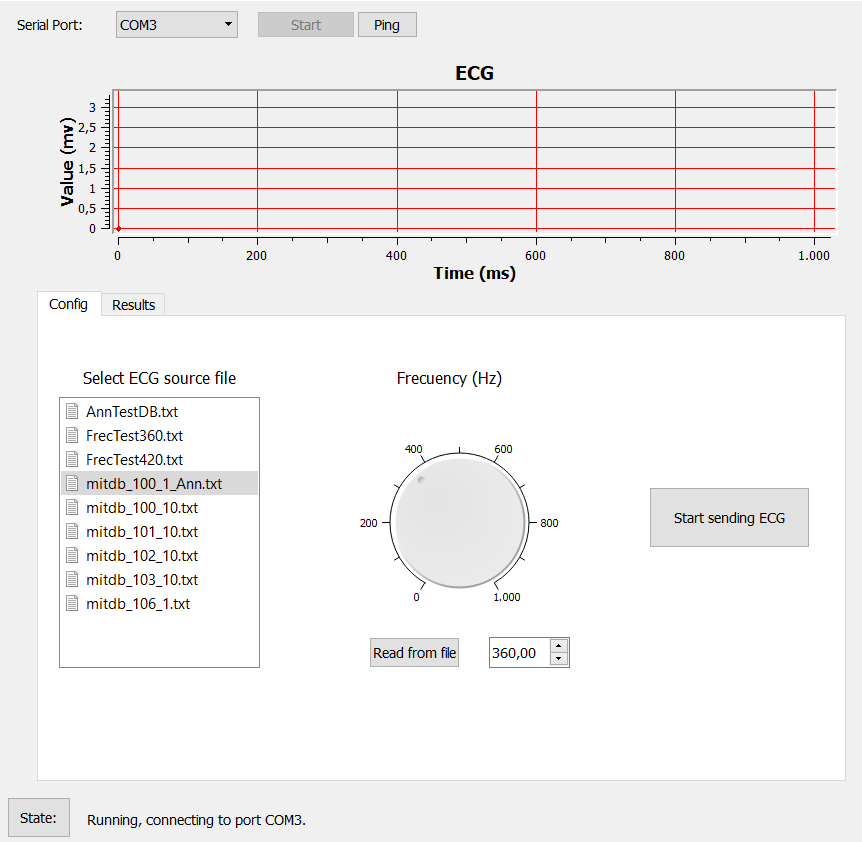
\includegraphics[width = \linewidth]{figuras/Config.PNG}
            \caption{Panel de usuario, configuración de la prueba.}
            \label{fig:EndConfig}
        \end{figure}
        
        \begin{figure}[H]
            \centering
                    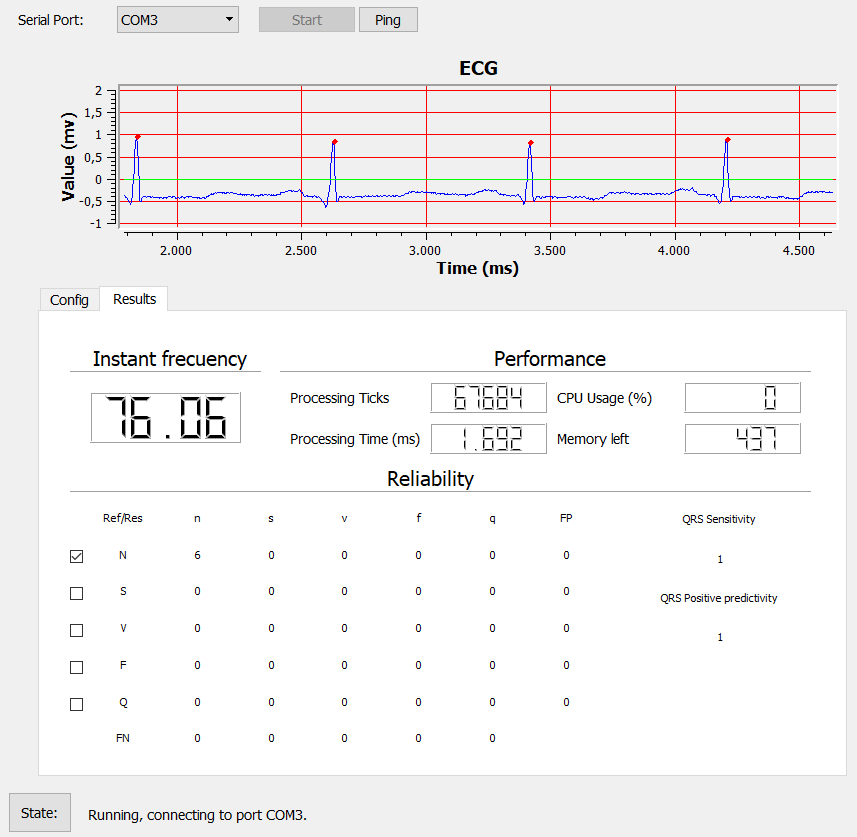
\includegraphics[width = \linewidth]{figuras/Results.PNG}
            \caption{Panel de usuario, resultados de la prueba.}
            \label{fig:EndResults}
        \end{figure}
        
    \clearpage
    \subsection{Pruebas}
    
    En esta iteración la única funcionalidad implementada susceptible de contener errores es la gestión del estado, necesaria para permitir al usuario detener y comenzar pruebas con diferentes muestras sin la necesidad de cerrar la sesión. Dado el carácter integral de esta funcionalidad resulta muy complicado realizar test unitarios, por lo que el método de prueba empleado ha sido simplemente un \textit{debug} intensivo probando exhaustivamente los casos posibles.
    
    \subsection{Conclusiones}
    
    Con esta iteración queda finalizado el desarrollo de este proyecto. El estado actual del sistema es estable, funcional y medianamente usable por lo que se pueden dar por finalizados todos los requisitos de alta prioridad establecidos al inicio del proyecto.
    
    A modo de resumen, a continuación se adjunta una tabla con los requisitos completos del proyecto, incluidos los que han surgido durante el desarrollo, y en ella se indica cuales se han satisfecho y cuales no.
    
    A continuación se adjunta una tabla con los requisitos completos del proyecto, incluidos los que han surgido durante el desarrollo, y en ella se indica cuales se han satisfecho y cuales no.

 \begin{scriptsize}
    \begin{longtable}{|p{0.05\linewidth}|p{0.20\linewidth}|p{0.25\linewidth}|p{0.25\linewidth}|p{0.02\linewidth}|p{0.02\linewidth}|}
        \caption{Requisitos Finales. \label{tab:RequisitosFinales}}\\
        \hline
        ID & Requisito & Descripción & Prueba & Prio & Fin \\ \hline
        \endfirsthead
        %
        \endhead
        %
        \hline
        \endfoot
        %
        \endlastfoot
        %
        1 & Panel de control & El proyecto debe disponer de un panel de usuario intuitivo para llevar a cabo las pruebas &  & 1 & \\ \hline
        1.1 & Introducir señal de prueba & Al panel de control se le debe proveer una señal de ECG formateada específicamente para poder probar el algoritmo deseado & Introducir un ECG extraído de alguna base de datos y comprobar que los valores de las muestras enviados se corresponden & 1 & Si\\ \hline
        1.2     & Observar la señal procesada & Al panel de control se le debe proveer de una gráfica de salida que muestre la señal procesada. & Observar las gráfica de salida y comprobar que los datos dibujados se corresponden con los de la lectura & 2 & Si\\ \hline 
        1.3     & Resultados & El panel de control debe ser capaz de mostrar al usuario los siguientes elementos: &  &  & \\ \hline
        1.3.1   & Frecuencia cardiaca instantánea & El panel deberá mostrar la frecuencia cardíaca instantánea medida por el algoritmo a testear. & Comprobar que el dato enviado por la aplicación de pruebas y el recibido por el panel son el mismo. La precisión de este no es un requisito pues dependerá del algoritmo con el que se esté trabajando. & 1 & Si\\ \hline
        1.3.2   & Picos detectados & El panel deberá mostrar información sobre los picos R detectados y sus posiciones, para facilitar la evaluación del algoritmo & Al igual que la prueba anterior, se debe garantizar la coherencia de los datos entre la aplicación y el panel de usuario. La validez de estos dependerá del algoritmo. & 1 & Si\\ \hline
        1.3.3   & Utilización del procesador & El panel deberá mostrar el uso de CPU que corresponde al proceso del algoritmo de la forma más aproximada posible & Introducir una función con una duración conocida y realizar la estimación. & 1 & Si\\ \hline
        1.3.4   & Utilización de memoria & El panel deberá mostrar el uso de memoria en cada momento de la forma más aproximada posible & Introducir una función que consuma una memoria conocida y realizar la medición & 1 & Si\\ \hline
        1.3.5   & Fiabilidad del algoritmo visual & El panel deberá mostrar la fiabilidad del algoritmo de forma visual superponiendo los picos detectados con la señal en la gráfica. & Asegurar que los datos recibidos y dibujados son los mismos. La validez de estos dependen del algoritmo. & 1 & Si\\ \hline
        1.3.6   & Fiabilidad del algoritmo contrastada & El panel deberá mostrar la fiabilidad del algoritmo en forma de tasa de falsos negativos y positivos. & Contrastar los resultados con las anotaciones de la base de datos. & 2 & Si\\ \hline
        1.4     & Resolución muestras & El panel deberá poder configurar la resolución empleada para las muestras en la aplicación, ofreciendo al usuario cierto control sobre la cantidad de muestras simultaneas con las que su algoritmo podrá trabajar. & Comprobar la resolución de los valores y la cantidad de muestras totales a procesar con un inspector en modo \textit{debug}.  & 2 & No\\ \hline
        1.5 & Selección de datos & El panel deberá proporcionar al usuario un mecanismo por el cual pueda seleccionar de forma fácil e intuitiva el conjunto de muestras a emplear sobre sus pruebas & Comprobar que las muestras son tomadas y que se puede modificar la entrada de forma intuitiva. & 1 & Si \\ \hline
        1.6 & Mecanismo de mensajes & El panel deberá proporcionar al usuario información de los errores que se produzcan, además de manejarlos adecuadamente. & Forzar todos los errores conocidos y observar que la información mostrada al usuario es coherente & 2 & No \\ \hline
        2       & Dispositivo de pruebas & El sistema debe disponer de un dispositivo encargado de simular el comportamiento de un supervisor de eventos cardíacos que emplee el algoritmo de detección de tasa cardíaca deseado. &  & 1 & \\ \hline
        2.1     & Protocolo de comunicación & La aplicación debe ser capaz de recibir los datos desde el panel de usuarios y devolver los resultados procesados. & El correcto funcionamiento del resto de requisitos es prueba suficiente para este. & 1 & Si\\ \hline
        2.2     & Entrada de datos en tiempo real & La aplicación debe enviar y recibir los datos en tiempo real para emular las condiciones de funcionamiento de un SEC. & Comprobar que la aplicación es capaz de recibir datos paulatinamente y devolverlos. & 1 & Si\\ \hline
        2.2.1   & Simular la entrada de datos por el ADC & La aplicación debe simular la adquisición de datos mediante un conversor analógico digital. Emulando el funcionamiento de un supervisor real. & Comprobar que el acceso a esos datos está controlado con un \textit{timer}, como si del ADC se tratase. & 2 & No\\ \hline
        2.3     & Interfaz para el algoritmo & La aplicación debe disponer de una interfaz, dentro de la cual se pueda encapsular el algoritmo de detección de tasa cardíaca que el usuario desee probar. & Implementar dos algoritmos diferentes sin necesidad de modificar nada fuera de la interfaz. & 1 & Si\\ \hline
        2.4     & Resolución muestras & La aplicación debe ser capaz de modificar la resolución empleada para las muestras en la aplicación, ofreciendo al usuario cierto control sobre la cantidad de muestras simultaneas con las que su algoritmo podrá trabajar. & Comprobar que el máximo de muestras almacenadas en el dispositivo varían en función de la calidad seleccionada en el panel de control. & 2 & No\\ \hline
        2.5 & Aislamiento del procesado de señal & La implementación del algoritmo del usuario debe quedar encapsulada para facilitar las mediciones.  & Comprobar que el mecanismo de encapsulado se está empleando correctamente.  & 2 & Si \\ \hline 
    \end{longtable}   
    \end{scriptsize}
    
    Si bien hay aspectos del sistema que pueden ser mejorados y elementos que pueden añadirse, están fuera del alcance de este proyecto, aunque se hablará sobre ellos en las conclusiones generales del proyecto en un apartado posterior, así como de las tareas no finalizadas.
\chapterend{}

% Capítulo 04.
%\input{Capitulo04.tex}

% Capítulo 05.
%\input{Capitulo05.tex}


%\part{Parte tercera.}
% !TEX root = A0.MiTFG.tex

\chapterbeginx{Conclusiones y líneas futuras}

Después de todo el desarrollo del proyecto, es pertinente hacer una
valoración final del mismo, respecto a los resultados obtenidos, las
expectativas o el resultado de la experiencia acumulada.

Esta sección es indispensable y en ella se ha de reflejar, lo más
claramente posible, las aportaciones del trabajo con unas conclusiones
finales.

Además, considerando también el estado de la técnica, se deben indicar
las posibles líneas futuras de trabajo, proponer otros puntos de vista
o cualquier otra sugerencia como postámbulo del presente trabajo, para
ser considerada por el lector o el tribunal evaluador.


\chapterend


% Anexos
%\part{Apéndices}

\appendix

%%%%%%%%%%%%%%%%%%%%%%%%%%%%%%%%%%%%%%%%%%%%%%%%%%%%%%%%%%%%%%%%%%%
%%% Documento LaTeX 																						%%%
%%%%%%%%%%%%%%%%%%%%%%%%%%%%%%%%%%%%%%%%%%%%%%%%%%%%%%%%%%%%%%%%%%%
% Título:		Apéndice A
% Autor:  	Ignacio Moreno Doblas
% Fecha:  	2014-02-01, actualizado 2019-11-11
% Versión:	0.5.0
%%%%%%%%%%%%%%%%%%%%%%%%%%%%%%%%%%%%%%%%%%%%%%%%%%%%%%%%%%%%%%%%%%%%

\pagestyle{fancy}
\fancyhead[LE,RO]{\thepage}
\fancyhead[RE]{Apéndice} %
\fancyhead[LO]{\nouppercase{\rightmark}}

\chapter{Instruction manual}

\minitoc

\section{General}

Welcome to the QRS detection algorithm benchmark platform for integrated and low power devices. This platform is created to make the performance and reliability checks much easier, providing an already implemented environment for testing the user's own algorithm without worrying too much about communications and the measure methods.

This document will guide the user one step at a time in order to accomplish a successful measurement of the algorithm, starting directly with the task of introducing the algorithm into the device.

\section{Introducing the algorithm}
For this task we recommend the usage of Code composer studio, but any IDE capable of compiling and assembling for a Tiva C series (TM4C123GXL) can be used.

There is a lot of stuff inside the project that is not interesting from a user's perspective, which is why the only explanation provided will be of the main files that are needed to introduce the algorithm, grouped in a single folder called “userEntry” and described in the following lines:

\begin{itemize}
    \item \textbf{userAlgorithm.h}: This is the header file, where the helper functions needed to implement the algorithm will be declared. Each one of them have to be placed under the ``User Function'' section. Any function declaration under other sections should not be erased.
    \item \textbf{userAlgorithm.c}: This is the main file where the algorithm will be implemented. One can create any number of helper functions for implementing it, but the main one, which will have the logic of the user's algorithm, needs to be QrsDetectionAlgorithm. This function is the one that will be called by the system. Also there is a function called EcgProcessingConfig that will be called once at the beginning of the benchmark and is perfect for placing all the initializations that the algorithm needs. 
\end{itemize}

All of this can be a little tricky at the beginning but there is a simple example already implemented just for providing a little more help.

\clearpage
\section{Configuring the test environment}
Once the algorithm is implemented in the benchmark device, it is the moment to open the user panel and start configuring the test.

\subsection{Downloading the samples}
This environment is tested with the Mit-BIH arrhythmia database, and ready to work with that data source. A Matlab function is provided with the system to download the desired signal and format it to the application standard. Theoretically, any source can be used as long as it is formatted for the app.

Once the file is created simply add it to the data folder. If it is the first source, the data folder will need to be created. Simply create a folder called “data” at the same level as the app.


\subsection{Configure the benchmark}
According to the image \ref{fig:EndConfigSteps} the configuration of the benchmark only needs 4 steps

\begin{enumerate}
    \item Connect the bench device though the serial port. The device has to be plugged before running the program. Once it is detected, just select it and click start. Ping can be used to check the connection.
    \item Next step is to select the input from one of the data files imported in the previous step. The file is selected simply by clicking on it.
    \item Before running the benchmark the frequency needs to be set. It can be done manually with the knob or automatically by clicking on the read from file button.
    \item Now we are ready to start, just click the Start sending ECG button and the benchmark should begin. For sending a new set of data, just return to the config label and click on the same button. This time the button will be called “Stop sending ECG”.
\end{enumerate}

\clearpage
\section{Interpreting the results}
Using the image \ref{fig:EndResultSteps} as a reference, the information displayed is:

\begin{enumerate}
    \item  A graphic showing the result of the algorithm in real time. The blue line represents the ECG and the red dots the detected R peaks. It can also use a green line that represents the threshold if the algorithm uses one.
    \item Instant frequency, measured between the last two detected beats.
    \item The performance is measured with four different values:
    \begin{itemize}
        \item Processing ticks, that represents the amount of cpu clock ticks used in each operation of the algorithm.
        \item Processing time, uses the processor clock frequency and the previously measured ticks to estimate the same measure in terms of milliseconds.
        \item CPU usage, is an estimation of the percentage of the CPU used, based on the processing ticks used by the algorithm and the data sampling rate.
        \item Memory left, is the minimum amount of stack space that has remained for the task since it was created.  The closer this value is to zero the closer it has come to overflowing its stack.
    \end{itemize}
    \item Annotations table based on the norm UNE-EN 60601-2-47:2002 \cite{Aenor2002}.
    \item Checkboxes to decide if an annotation is taken into consideration for the Reliability or not. All beats found in the database with an unchecked annotation will be treated as an N beat. This is useful for certain algorithms that do not differentiate some types of beats. 
    \item Final measures of reliability, calculated following the guidelines of the norm UNE-EN 60601-2-47:2002 \cite{Aenor2002}.

\end{enumerate}

\begin{figure}[H]
            \centering
                    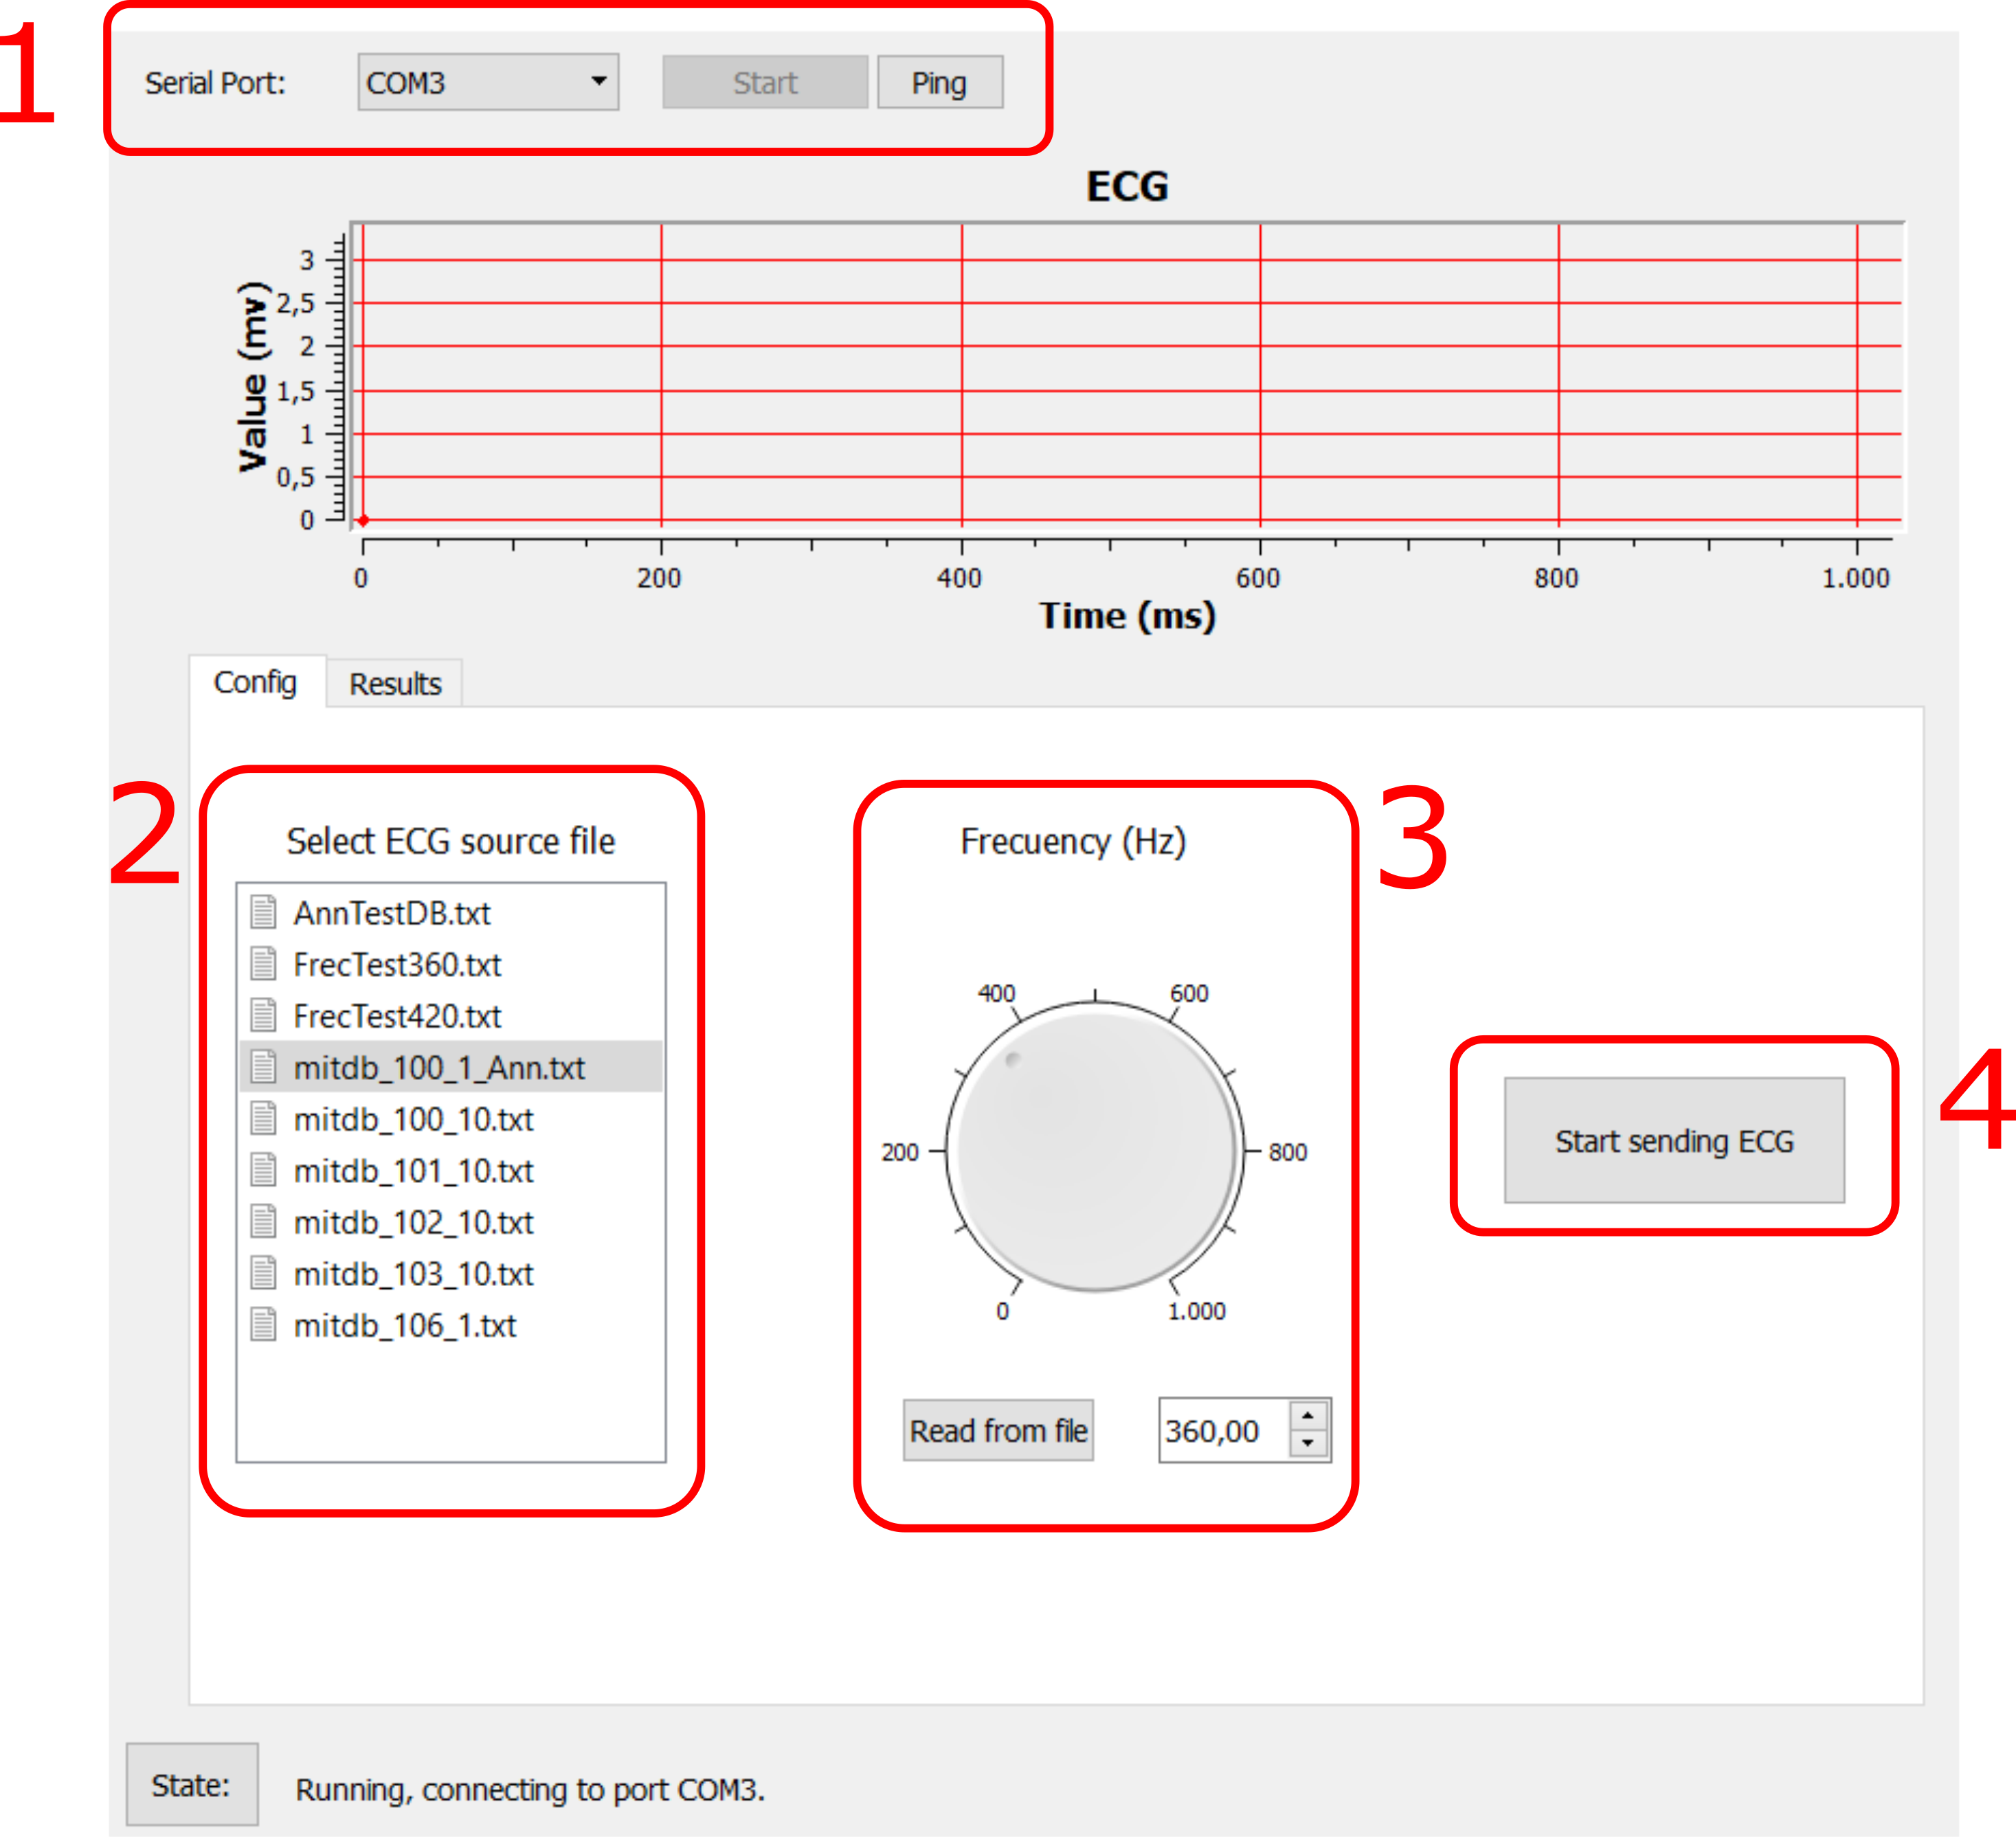
\includegraphics[width = \linewidth]{figuras/configSteps.png}
            \caption{User panel, config label with configuration steps.}
            \label{fig:EndConfigSteps}
        \end{figure}
        
        \begin{figure}[H]
            \centering
                    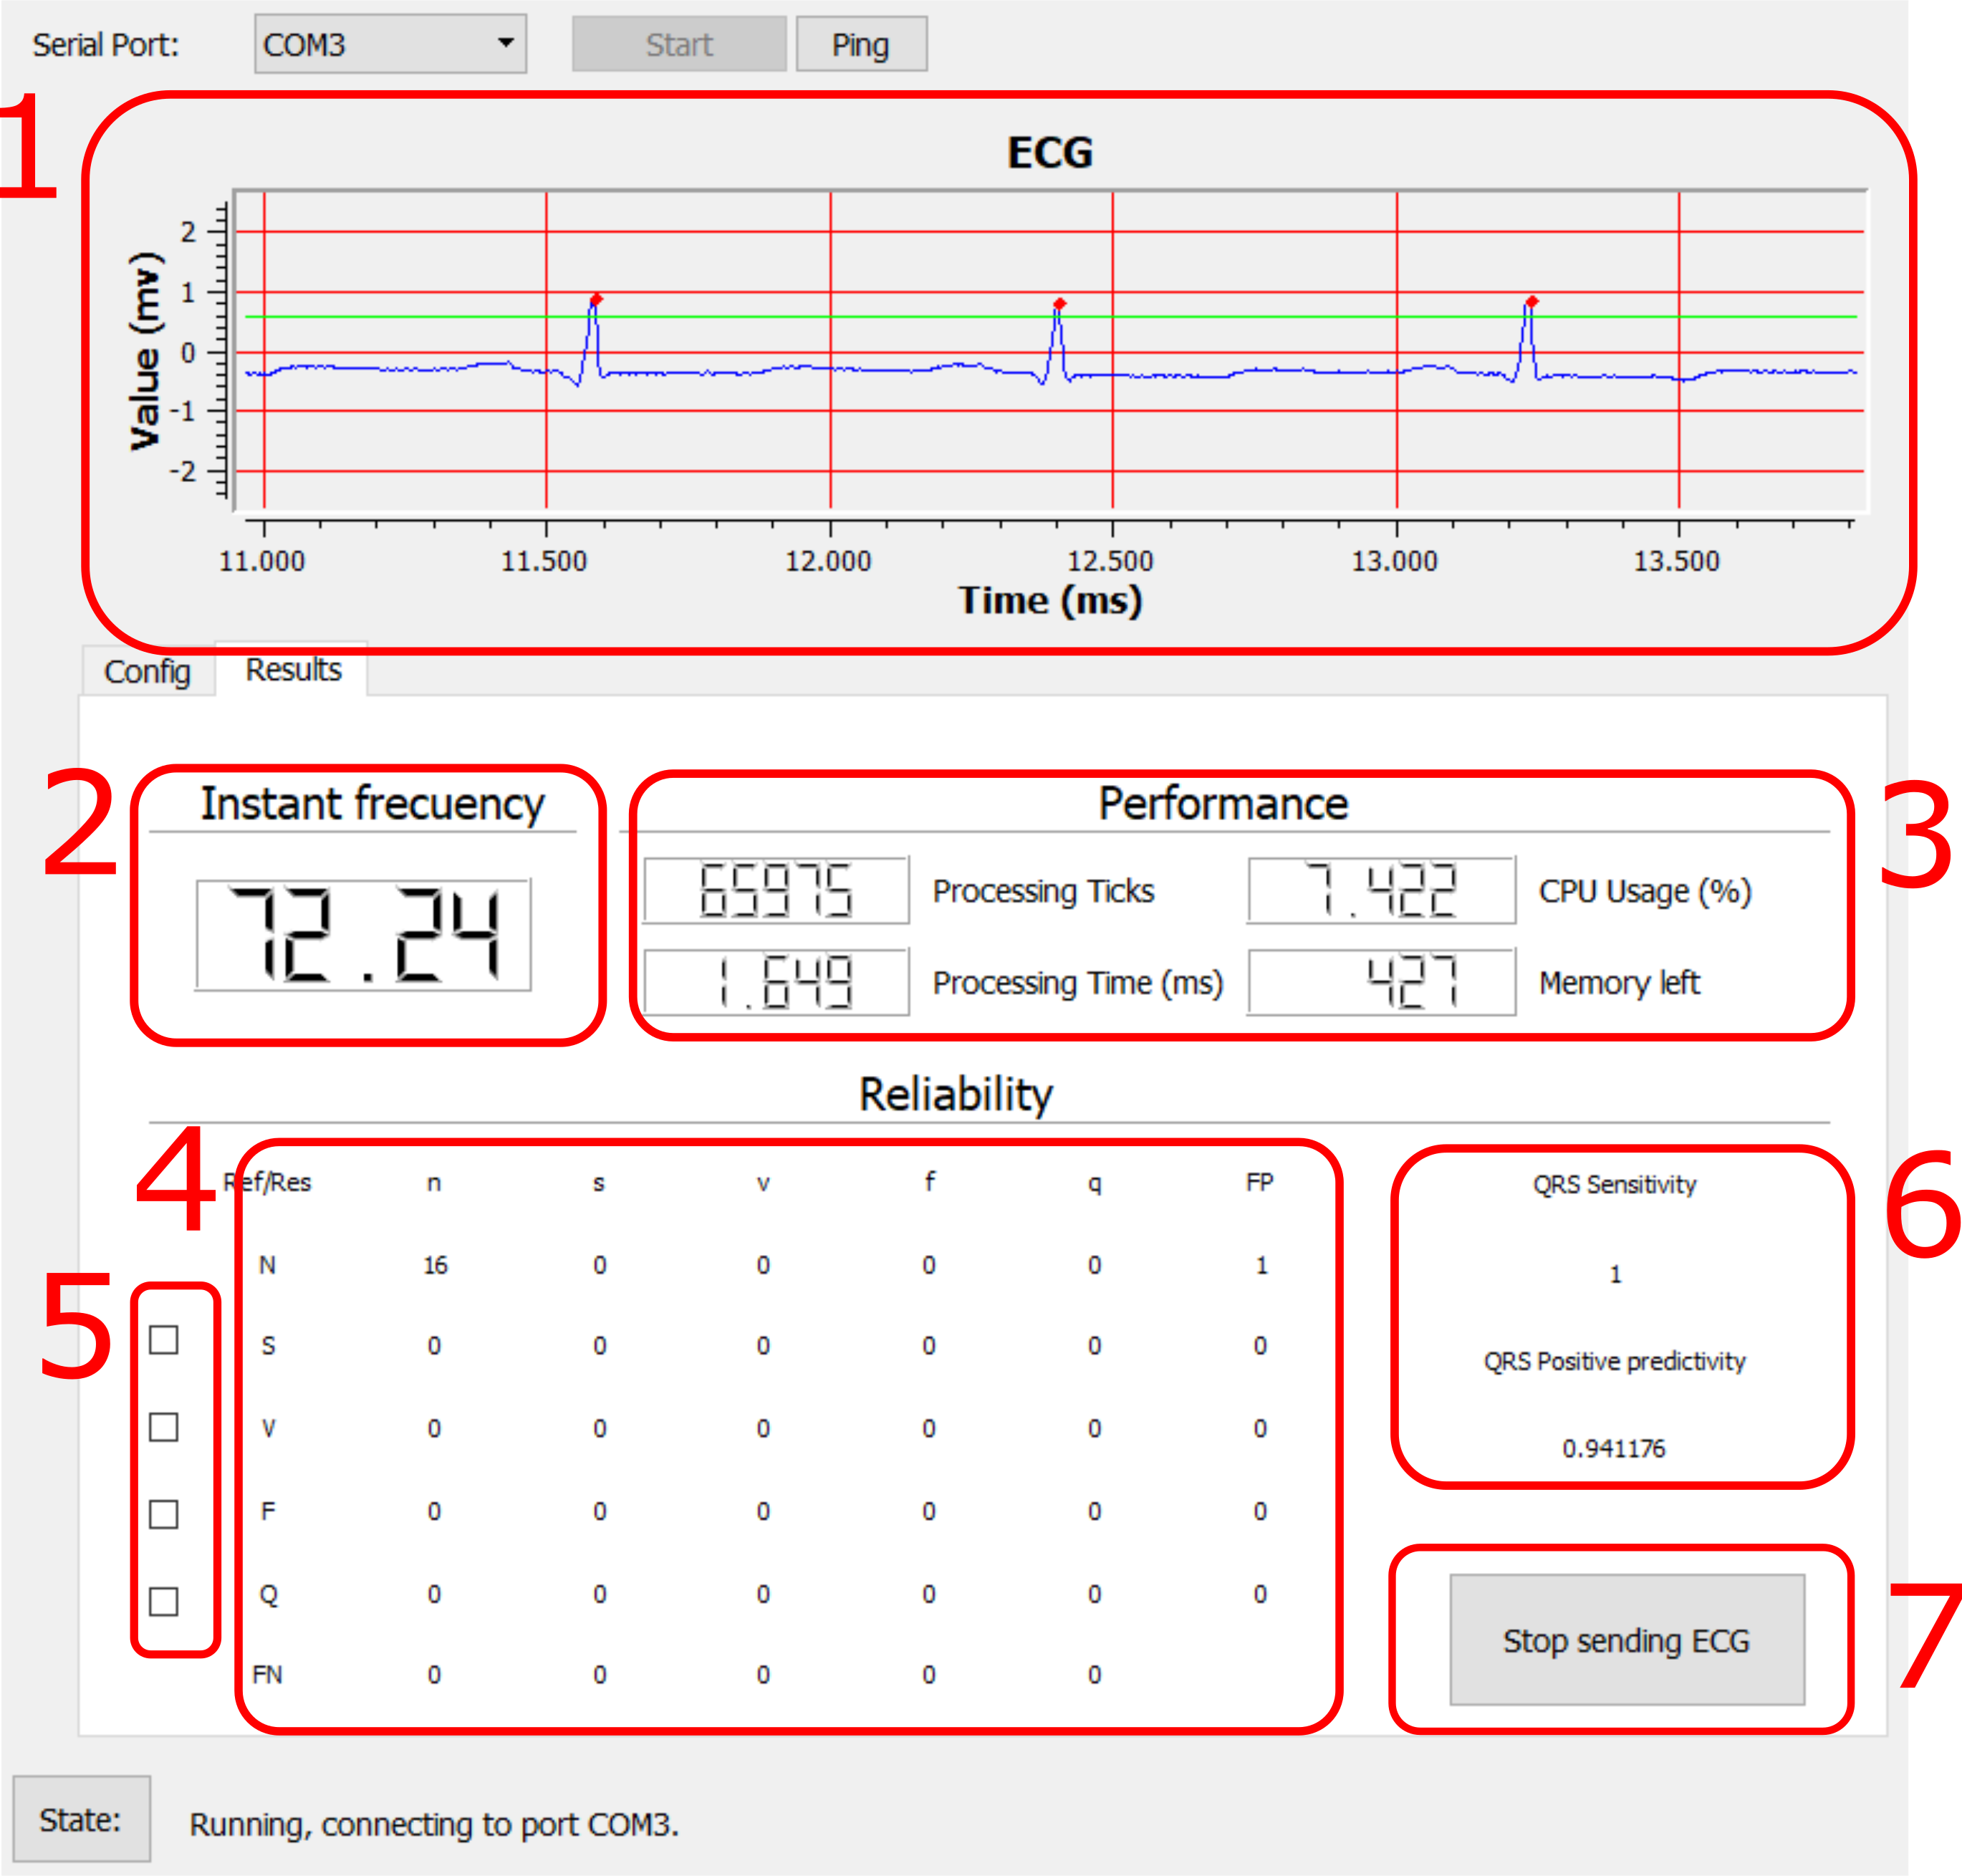
\includegraphics[width = \linewidth]{figuras/resultSteps.png}
            \caption{User panel, result label with helper index.}
            \label{fig:EndResultSteps}
        \end{figure}

\chapterend


%%%%%%%%%%%%%%%%%%%%%%%%%%%%%%%%%%%%%%%%%%%%%%%%%%%%%%%%%%%%%%%%%%%%
%%% Documento LaTeX 																						%%%
%%%%%%%%%%%%%%%%%%%%%%%%%%%%%%%%%%%%%%%%%%%%%%%%%%%%%%%%%%%%%%%%%%%
% Título:		Apéndice A
% Autor:  	Ignacio Moreno Doblas
% Fecha:  	2014-02-01, actualizado 2019-11-11
% Versión:	0.5.0
%%%%%%%%%%%%%%%%%%%%%%%%%%%%%%%%%%%%%%%%%%%%%%%%%%%%%%%%%%%%%%%%%%%%

\pagestyle{fancy}
\fancyhead[LE,RO]{\thepage}
\fancyhead[RE]{Apéndice} %
\fancyhead[LO]{\nouppercase{\rightmark}}

\chapter{Anexos}

\minitoc

\section{Tests Unitarios}

\subsection{Descripción}

El concepto test unitario hace referencia a una serie de pruebas realizadas sobre un único componente del sistema. La finalidad de esto es asegurar que cada componente cumple con sus funciones de la forma esperada. Generalmente cada componente, o unidad, solo posee unas pocas entradas y una única salida y el test consiste en verificar todos los casos posibles con diferentes entradas fijas que poseen respuestas conocidas.

Implementando las pruebas de esta forma se consigue facilitar la tarea de mantener el código durante el desarrollo, ya que si alguna vez se modifica la lógica de alguna unidad, se vuelven a ejecutar los tests unitarios para comprobar si el componente sigue funcionando según lo esperado, evitando tener que realizar pruebas nuevas cada vez que se modifica un componente.

Además ofrece otros beneficios como la modularidad del código, agiliza el desarrollo a largo plazo, el código se vuelve más sencillo de debugear y evita que los bugs se propaguen a fases más avanzadas del desarrollo.

\subsection{Implementación en QT}

El framework de QT posee las herramientas necesarias para realizar pruebas unitarias de forma nativa. Sin embargo es necesario realizar ciertos pasos previos para preparar el proyecto y tener en cuenta ciertas consideraciones.

\subsubsection{Configurar el proyecto de QT}

Primeramente es necesario crear un proyecto de QT multicarpeta, ya que los tests se implementan en un proyecto separado de la aplicación principal, este proyecto será llamado de ahora en adelante como el proyecto raíz.

Para esto es necesario crear un directorio y generar a mano el ``projectName.pro'' del proyecto fijando el valor del campo ``TEMPLATE'' a subdirs. Dado que los proyectos de QT son carpetas, hay que añadir los subdirectorios al fichero quedando de forma similar al extracto (TODO: Referencia del .pro). 

(Extracto del .pro)

En caso de poseer ya un proyecto previo, se puede introducir dentro del proyecto raíz simplemente copiando la carpeta en el interior, asegurando que coincide con el subdirectorio que se ha configurado.

\subsubsection{Crear los proyectos de test}

El proceso para generar los proyectos de test es simple gracias a las herramientas que ofrece QT creator.

Abriendo el proyecto raíz con la aplicación QT creator, hay que generar un subproyecto. Para ello la forma más directa es hacer click derecho sobre el proyecto raíz y seleccionar en el menú la opción ``New subproject''. En la ventana emergente se selecciona ``Other Project/Auto Test Project''.

Ahora solo es necesario seguir los pasos indicados rellenando los campos necesarios. los campos que no se mencionan a continuación no es necesario modificarlos.

\begin{itemize}
    \item Name: Nombre del proyecto, generalmente es buena práctica empezar por ``tst''.
    \item Test case name: El nombre del caso a testear, generalmente el componente, la recomendación es emplear un subproyecto por cada componente.
    \item Marcar la casilla Generate initialization and cleanup code.
    \item Seleccionar los kits necesarios, generalmente los mismos que use el proyecto principal.
\end{itemize}

Este proceso habrá generado un nuevo proyecto (Y su carpeta) y habrá introducido el subdirectorio directamente en el ``.pro'' del proyecto raíz. Para evitar que los proyectos de test se incluyan en el proceso de compilación del modo release se puede añadir el comando ``CONFIG(debug, debug|release)'', quedando finalmente el fichero de forma similar al extracto (TODO: Extracto fichero .pro con subdirs de test)

\subsubsection{Configurar los proyectos de test}





\chapterend


%%%%%%%%%%%%%%%%%%%%%%%%%%%%%%%%%%%%%%%%%%%%%%%%%%%%%%%%%%%%%%%%%%%%
%%% Documento LaTeX 																						%%%
%%%%%%%%%%%%%%%%%%%%%%%%%%%%%%%%%%%%%%%%%%%%%%%%%%%%%%%%%%%%%%%%%%%
% Título:		Apéndice A
% Autor:  	Ignacio Moreno Doblas
% Fecha:  	2014-02-01, actualizado 2019-11-11
% Versión:	0.5.0
%%%%%%%%%%%%%%%%%%%%%%%%%%%%%%%%%%%%%%%%%%%%%%%%%%%%%%%%%%%%%%%%%%%%

\pagestyle{fancy}
\fancyhead[LE,RO]{\thepage}
\fancyhead[RE]{Apéndice} %
\fancyhead[LO]{\nouppercase{\rightmark}}

\chapter{Horas de desarrollo}

\minitoc
\section{Total}

Para el desarrollo de este proyecto se han empleado un total aproximado de \textbf{303 horas}, repartidas entre el desarrollo del sistema, las sesiones de control y la redacción del documento.

\section{Desglose}

A continuación se presenta un desglose de las horas empleadas durante el desarrollo del proyecto.
En el tiempo asignado a cada tarea va incluido el tiempo invertido en el documento correspondiente a dicha tarea.

\begin{itemize}
    \item \textbf{Estudio previo e introducción:} 40 horas.
    \item \textbf{Especificaciones:} 18 horas.
    \item \textbf{Iteración inicial:} 12 horas.
    \item \textbf{Primera iteración:} 30 horas.
    \begin{itemize}
        \item Introducción de las señales de prueba: 10 horas.
        \item Envío de datos provenientes de la base de datos en tiempo real al dispositivo de pruebas: 12 horas. 
        \item Pruebas: 8 horas.
    \end{itemize}
    \item \textbf{Segunda iteración:} 35 horas.
    \begin{itemize}
        \item Implementar un mecanismo por el que seleccionar el fichero de entrada: 10 horas.
        \item Implementar la interfaz para los algoritmos de detección: 9 horas. 
        \item Mostrar los resultados del análisis en el panel de usuario: 6 horas.
        \item Pruebas: 10 horas.
    \end{itemize}
    \item \textbf{Tercera iteración:} 34 horas.
    \begin{itemize}
        \item Aislamiento del procesado de señales en una tarea exclusiva.: 5 horas.
        \item Extraer las medidas de rendimiento del sistema operativo: 16 horas. 
        \item Mostrar dichas medidas en el panel de usuario de QT: 5 horas.
        \item Pruebas: 8 horas.
    \end{itemize}
    \item \textbf{Cuarta iteración:} 74 horas.
    \begin{itemize}
        \item Estudio de la norma Une-en 60601-2-47:2002: 6 horas.
        \item Extraer las anotaciones de la base de datos y añadirlas al fichero de entra-da: 5 horas. 
        \item Preparar el dispositivo de pruebas para transmitir anotaciones junto a la detección de los latidos: 3 hora.
        \item Modificar el algoritmo de detección implementado en la segunda iteración para enviar anotaciones: 5 hora.
        \item  Crear un modelo de almacenamiento para las anotaciones que facilite la implementación de la norma: 16 horas.
        \item Implementar el control de las anotaciones en el panel de usuario: 12 horas.
        \item Implementar las ecuaciones de cálculo de fiabilidad descritas en la norma: 6 horas.
        \item Mostrar al usuario los resultados de la validación del algoritmo: 5 horas.
        \item Pruebas: 16 horas.
    \end{itemize}
    \item \textbf{Quinta iteración:} 30
    \begin{itemize}
        \item Limpieza de código y asegurar coherencia en la nomenclatura: 8 horas.
        \item Añadir comentarios necesarios para facilitar la lectura del código y su mantenimiento: 8 horas. 
        \item  Mejorar la apariencia visual del panel y mejorar su usabilidad en la medida de lo posible: 8 horas.
        \item Estimación matemática del porcentaje de uso de la CPU: 2 horas.
        \item Pruebas: 4 horas.
    \end{itemize}
    \item \textbf{Repaso y revisión del documento:} 16 horas
    \item \textbf{Reuniones y sesiones de control:} 14 horas
\end{itemize}

\chapterend

% Formato de documento en la parte final.
\backmatter
%Hace que los capítulos y títulos nivel inferior no aparezcan numerados (lo que es ideal para conclusiones o notas finales).

% Bibliografía
%%%%%%%%%%%%%%%%%%%%%%%%%%%%%%%%%%%%%%%%%%%%%%%%%%%%%%%%%%%%%%%%%%%
%%% Documento LaTeX 																						%%%
%%%%%%%%%%%%%%%%%%%%%%%%%%%%%%%%%%%%%%%%%%%%%%%%%%%%%%%%%%%%%%%%%%%
% Título:		Bibliografía
% Autor:  	Ignacio Moreno Doblas
% Fecha:  	2014-02-01, actualizado 2019-11-11
% Versión:	0.5.0
%%%%%%%%%%%%%%%%%%%%%%%%%%%%%%%%%%%%%%%%%%%%%%%%%%%%%%%%%%%%%%%%%%%%

% Encabezamiento %
\pagestyle{fancy}
\fancyhead[LE,RO]{\thepage}
\fancyhead[RE,LO]{Bibliografía}

%Inclusión de bibliografía%
\bibliography{E2.Bibliografia} %Úsese el nombre del fichero sin extensión

%Inclusión en el índice (Tabla de contenidos)
\addcontentsline{toc}{chapter}{Bibliografía}

%Formateo de estilo de bibliografía
% Otros formatos: plain, unsrt, abbrv
%  plain: las entradas se ordenan alfabéticamente y se etiquetan con un número (p.ej., [1])
% unsrt: igual que plain, pero aparecen en orden de citación.
% alpha: el etiquetado se hace por autor y año de publicación (p.ej., [Knu66]).
% abbrv: igual que alpha, pero más abreviado.
\bibliographystyle{plain}

%Impresión de todas las entradas bibliográficas aunque no estén citadas
%\nocite{*}

\chapterend


% Índice alfabético%
%%%%%%%%%%%%%%%%%%%%%%%%%%%%%%%%%%%%%%%%%%%%%%%%%%%%%%%%%%%%%%%%%%%
%%% Documento LaTeX 																						%%%
%%%%%%%%%%%%%%%%%%%%%%%%%%%%%%%%%%%%%%%%%%%%%%%%%%%%%%%%%%%%%%%%%%%
% Título:		Glosario (index)
% Autor:  	Ignacio Moreno Doblas
% Fecha:  	2014-02-01, actualizado 2019-11-11
% Versión:	0.5.0
%%%%%%%%%%%%%%%%%%%%%%%%%%%%%%%%%%%%%%%%%%%%%%%%%%%%%%%%%%%%%%%%%%%%

\pagestyle{fancy}
\fancyhead[LE,RO]{\thepage}
\fancyhead[RE,LO]{Glosario} 

\printindex

%Example 	Index Entry 	Comment
%\index{hello} 	hello, 1 	Plain entry
%\index{hello!Peter} 	  Peter, 3 	Subentry under 'hello'
%\index{Sam@\textsl{Sam}} 	Sam, 2 	Formatted entry
%\index{Lin@\textbf{Lin}} 	Lin, 7 	Same as above
%\index{Jenny|textbf} 	Jenny, 3 	Formatted page number
%\index{Joe|textit} 	Joe, 5 	Same as above
%\index{ecole@\'ecole} 	école, 4 	Handling of accents
%\index{Peter|see{hello}} 	Peter, see hello 	Cross-references
%\index{Jen|seealso{Jenny}} 	Jen, see also Jenny 	Same as above


\chapterend


\end{document}
